\documentclass[notoc]{tufte-book}    % `notoc` suppresses TL custom TOC, reverts to standard LaTeX

\hyphenation{HMMER}

\begin{titlepage}
{\Large

\vspace*{\fill}

\noindent
{\Huge {INFERNAL User's Guide}} \vspace{-8.0pt} \\ 
\rule[2pt]{\textwidth}{1pt} \\
\hspace*{\fill} {\large {Sequence analysis using profiles of RNA
sequence and secondary structure consensus} \\ }

\vspace*{\fill}

\begin{center}
\url{http://eddylab.org/infernal}\\
Version 1.1.4; Dec 2020 \\ 

\vspace*{\fill}

Eric Nawrocki and Sean Eddy\\
for the INFERNAL development team\\
\url{https://github.com/EddyRivasLab/infernal/}
\end{center}

\vspace*{\fill}

}
\end{titlepage}
                    % definitions for \maketitle 
\bibliographystyle{unsrtnat-brief}   % customized natbib unsrtnat. Abbrev 3+ authors to ``et al.'' 

\begin{document}
\setcounter{tocdepth}{2}             % 0=chapters 1=sections 2=subsections 3=subsubsections? 4=paragraphs
\newcommand{\UNIrelease}{2020\_05}
\newcommand{\UNInseq}{563,552}

\newcommand{\HMMERversion}{3.3.2}
\newcommand{\HMMERdate}{Nov 2020}

\newcommand{\BGLnseq}{4}
\newcommand{\BGLalen}{171}
\newcommand{\BGLmlen}{149}
\newcommand{\BGLgaps}{22}
\newcommand{\BGLeffn}{0.96}
\newcommand{\BGLre}{0.589}

\newcommand{\HMMERfmtversion}{f}
\newcommand{\HMMERsavestamp}{[3.3.2 | Nov 2020]}

\newcommand{\SGUevalue}{4.9e-65}
\newcommand{\SGUbitscore}{223.2}
\newcommand{\SGUbias}{0.1}
\newcommand{\SGUorigscore}{223.3}
\newcommand{\SGUdombitscore}{223.0}
\newcommand{\SGUseqname}{HBB\_GORGO}
\newcommand{\SGUmsvpass}{3.7}
\newcommand{\SGUbiaspass}{17002}
\newcommand{\SGUvitpass}{2323}
\newcommand{\SGUfwdpass}{1129}
\newcommand{\SGUelapsed}{0.9}

\newcommand{\SFSevalue}{5.6e-57}
\newcommand{\SFSbitscore}{176.4}
\newcommand{\SFSdomevalue}{2.3e-16}
\newcommand{\SFSdombitscore}{46.2}
\newcommand{\SFSexpdom}{9.8}
\newcommand{\SFSndom}{9}

\newcommand{\SFSmaxdom}{7}
\newcommand{\SFSmaxdomu}{5}
\newcommand{\SFSmaxsc}{46.2}
\newcommand{\SFSievalue}{2.3e-16}
\newcommand{\SFSuievalue}{1.3e-10}
\newcommand{\SFSdomZ}{794}
\newcommand{\SFSucevalue}{1.9e-13}
\newcommand{\SFSaidx}{1}
\newcommand{\SFSascore}{-1.9}
\newcommand{\SFSaevalue}{0.24}
\newcommand{\SFSauevalue}{191}
\newcommand{\SFSacoords}{395-410}
\newcommand{\SFSbidx}{6}
\newcommand{\SFSbscore}{0.4}
\newcommand{\SFSbevalue}{0.045}
\newcommand{\SFSbuevalue}{35.7}
\newcommand{\SFSbcoords}{1742-1769}
\newcommand{\SFSainsig}{4.6}
\newcommand{\SFSbinsig}{8.9}

\newcommand{\JHUninc}{955}
\newcommand{\JHUnsig}{955}

\newcommand{\NMHafrom}{302390}
\newcommand{\NMHato}{302466}
\newcommand{\NMHbfrom}{302466}
\newcommand{\NMHbto}{302389}
\newcommand{\NMHnres}{660000}
\newcommand{\NMHntop}{330000}
\newcommand{\NMHnssv}{73493}
\newcommand{\NMHfracssv}{11.1}
\newcommand{\NMHnbias}{49311}
\newcommand{\NMHfracbias}{7.5}
\newcommand{\NMHnvit}{4022}
\newcommand{\NMHfracvit}{0.6}
\newcommand{\NMHnfwd}{1562}
    % snippets captured from output, by gen-inclusions.py 

\maketitle

\newpage
\vspace*{\fill}
\begin{flushleft}

\vspace{2em}
Copyright (C) 2020 Howard Hughes Medical Institute.

\vspace{2em}
Infernal and its documentation are freely distributed under the 
3-Clause BSD open source license. For a copy of the license, see
\url{http://opensource.org/licenses/BSD-3-Clause}.

\vspace{2em}
Infernal development is supported by the Intramural Research Program
of the National Library of Medicine at the US National Institutes of
Health, and also by the National Human Genome Research Institute of
the US National Institutes of Health under grant number
R01HG009116. The content is solely the responsibility of the authors
and does not necessarily represent the official views of the National
Institutes of Health.

\end{flushleft}






\begin{adjustwidth}{}{-1in}          % TL \textwidth is quite narrow. Expand it manually for TOC and man pages.
\tableofcontents                     
\end{adjustwidth}

\section{Introduction}
\label{section:introduction}
\setcounter{footnote}{0}

Infernal is used to search sequence databases for homologs of
structural RNA sequences, and to make sequence- and structure-based
RNA sequence alignments. Infernal builds a \emph{profile} from a
structurally annotated multiple sequence alignment of an RNA family
with a position-specific scoring system for substitutions, insertions,
and deletions. Positions in the profile that are basepaired in the
  h consensus secondary structure of the alignment are modeled as
dependent on one another, allowing Infernal's scoring system to
consider the secondary structure, in addition to the primary sequence,
of the family being modeled. Infernal profiles are probabilistic
models called ``covariance models'', a specialized type of stochastic
context-free grammar (SCFG) \citep{Lari90}.

Compared to other alignment and database search tools based only on
sequence comparison, Infernal aims to be significantly more accurate
and more able to detect remote homologs because it models sequence
and structure. But modeling structure comes at a high computational
cost, and the slow speed of CM homology searches has been a serious
limitation of previous versions. With
version 1.1, typical homology searches are now about 100x faster,
thanks to the incorporation of accelerated HMM methods from the HMMER3
software package (\url{http://hmmer.org}), making Infernal a much more
practical tool for RNA sequence analysis.

\subsection{How to avoid reading this manual}

If you're like most people, you don't enjoy reading documentation.
You're probably thinking: \pageref{manualend} pages of documentation,
you must be joking! I just want to know that the software compiles,
runs, and gives apparently useful results, before I read some
\pageref{manualend} exhausting pages of someone's documentation. For
cynics that have seen one too many software packages that don't work:

\begin{itemize}
\item Follow the quick installation instructions on page
      \pageref{section:installation}. An automated test suite
      is included, so you will know immediately if something
      went wrong.\footnote{Nothing should go wrong.}
\item Go to the tutorial section on page
\pageref{section:tutorial}, which walks you through some examples of
using Infernal on real data.
\end{itemize}

Everything else, you can come back and read later.

\subsection{What covariance models are}

Covariance models (CMs) are statistical models of structurally
annotated RNA multiple sequence alignments, or even of single
sequences and structures. CMs are a specific formulation of profile
stochastic context-free grammars (profile SCFG), which were introduced
independently by Yasu Sakakibara in David Haussler's
group \citep{Sakakibara94c} and by Sean Eddy and Richard
Durbin \citep{Eddy94}. CMs are closely related to profile hidden Markov
models (profile HMMs) commonly used for protein sequence analysis, but
are more complex. CMs and profile HMMs both capture position-specific
information about how conserved each column of the alignment is, and
which residues are likely. However, in a profile HMM each position of
the profile is treated independently, while in a CM basepaired
positions are dependent on one another.  The dependency between paired
positions in a CM enables the profile to model \emph{covariation} at
these positions, which often occurs between basepaired columns of
structural RNA alignments. For many of these basepairs, it is not the
specific nucleotides that make up the pair that is conserved by
evolution, but rather that the pair maintain Watson-Crick
basepairing. The added signal from covariation can be significant when
using CMs for homology searches in large
databases. Section~\ref{section:cmbuild} of this guide explains how a
CM is constructed from a structurally annotated alignment using a toy
example. 

CMs do have important limitations though. For example, a CM can only
model what is called a ``well-nested'' set of basepairs. Formally, in
a well-nested set of basepairs there are no two basepairs between
positions $i:j$ and $k:l$ such that $i<k<j<l$. CMs cannot model
pseudoknots in RNA secondary structures. Additionally, a CM only
models a single consensus structure for the family it models. 

\subsection{Applications of covariance models}

Infernal can be useful if you're intereseted in a particular RNA
family. Imagine that you've carefully collected and aligned a set of
homologs and have a predicted (or known) secondary structure for the
family. Homology searches with BLAST using single sequences from your
set of homologs may not reveal any additional homologs in sequence
databases. You can build a CM from your alignment and redo your search
using Infernal (this time only a single search) and you may find new
homologs thanks to the added power of the profile-based sequence and
structure scoring system of CMs. The Rfam database \citep{Gardner11}
essentially does just this, but on a much larger scale. The Rfam
curators maintain about 2000 RNA families, each represented by a
multiple sequence alignment (called a \emph{seed} alignment) and a CM
built from that alignment. Each Rfam release involves a search through
a large EMBL-based nucleotide sequence database with each of the CMs
which identifies putative structural RNAs in the database. The
annotations of these RNAs, as well as the CMs and seed alignments are
freely available.

Automated genome annotation of structural RNAs can be performed with
Infernal and a collection of CMs from Rfam, by searching
through the genome of interest with each CM and collecting information
on high-scoring hits. Previous versions of Infernal were too slow to
be incorporated into many genome annotation pipelines, but we're
hoping the improved speed of version 1.1 changes this.

Another application is the automated construction and maintenance of
large sequence- and structure-based multiple alignment databases.  For
example, the Ribosomal Database Project uses CMs of 16S small subunit
ribosomal RNA (16S SSU rRNA) to maintain alignments of millions of 16S
sequences \citep{Cole09}. The CMs (one archaeal 16S and one bacterial
16S model) were built from training alignments of only a few hundred
representative sequences. The manageable size of the training
alignments means that they can be manually curated prior to building
the model. Rfam is another example of this application too because
Rfam creates and makes available multiple alignments (called \emph{full}
alignments) of all of the hits from the database its curators believe
to be real RNA homologs.

Infernal can also be used to determine what types of RNAs exist in a
particular sequence dataset. Suppose you're performing a metagenomics
analysis and have collected sequences from an exotic environmental
sample. You can download all the CMs from Rfam and use Infernal to
search through all your sequences for high-scoring hits to the
models. The types of structural RNAs identified in your sample can be
informative as to what types of organisms are in your sample, and what
types of biological processes they're carrying out. Version 1.1
includes a new program called \prog{cmscan} which is designed for just
this type of analysis.

\subsection{Infernal and HMMER, CMs and profile HMMs}

Infernal is closely related to HMMER. In fact, HMMER is used as a
library within the Infernal codebase. This allows Infernal to use the
highly optimized profile HMM dynamic programming implementations in
HMMER to greatly accelerate its homology searches. Also, the design
and organization of the Infernal programs (e.g. \ccode{cmbuild},
\ccode{cmsearch}, \ccode{cmalign}) follows that in HMMER
(\ccode{hmmbuild}, \ccode{hmmsearch}, \ccode{hmmalign}). And there are
many functions in Infernal that are based on analogous ones in
HMMER. The formatting of output is often very similar between
these two software packages, and the user guide's are even organized
and written in a similar (and, in some places, identical) way. 

This is, of course, on purpose. Since both packages are developed in
the same lab, consistency simplifies the development and maintenance
of the code, but we also do it to make the software (hopefully) easier
to use (someone familiar with using HMMER should be able to pick up
and use Infernal very easily, and vice versa). However, Infernal
development tends to lag behind HMMER development as new ideas and
algorithms are applied to the protein or DNA world with profile HMMs,
and then later extended to CMs for use on RNAs.
%Some of the current features of HMMER are on
%the 00TODO list for Infernal (and by the time they're implemented they
%will have been replaced on that list).

This consistency is possible because profile HMMs and covariance
models are related models with related applications.  Profile HMMs are
profiles of the conserved sequence of a protein or DNA family and CMs
are profiles of the conserved sequence \emph{and} well-nested
secondary structure of a structural RNA family. Applications of
profile HMMs include annotating protein sequences in proteomes or
protein sequence database and creating multiple alignments of protein
domain families. And similarly applications of CMs include annotating
structural RNAs in genomes or nucleotide sequence databases and
creating sequence- and structure-based multiple alignments of RNA.
The crucial difference is that CMs are able to model dependencies
between a set of well-nested (non-pseudoknotted) basepaired positions
in a structural RNA family. The statistical signal inherent in these
dependencies is often significant enough to make modeling the family
with a CM a noticeably more powerful approach than modeling the family
with a profile HMM.

\subsection{What's new in Infernal 1.1}

The most important difference between version 1.1 and the previous
version (1.0.2) is the improved search speed that results from a new
filter pipeline. The pipeline is explained more in
section~\ref{section:pipeline}. Another important change is the
introduction of the \prog{cmscan} program, for users who want to know
what structural RNAs are present in a collection of sequences, such as
a metagenomics dataset\footnote{\prog{cmscan} is similar to
\prog{cmsearch} but is more convenient for some applications. One
difference between the two programs is that results from \prog{cmscan}
are organized per-sequence instead of per-model.}. Another new feature
of version 1.1 is better handling of truncated RNAs, for which part of
one or both ends of the RNA is missing due to a premature end of the
sequence \citep{KolbeEddy09}. These types of fragmentary sequences are
common in whole genome shotgun sequencing datasets. While previous
versions of Infernal were prone to misalignment of these sequences,
version 1.1 includes implementations of CM search and alignment
algorithms specialized for truncated sequences \citep{KolbeEddy09} in
\prog{cmsearch}, \prog{cmscan} and \prog{cmalign}.

Model parameterization has changed in several minor ways. Mixture
Dirichlet priors for emissions and single component Dirichlet priors
for transitions have been reestimated using larger and more diverse
datasets than the ones the previous priors were derived from
(discussed in \citep{NawrockiEddy07}). Also, the definition of match
and insert columns, previously determined by a simple majority rule
using absolute counts (columns in which $\geq 50\%$ of columns include
residues were match, all others were insert), now use \emph{weighted}
counts (and same $>=50\%$ rule) after a sequence weighting algorithm
is applied. And inserts before the first and after the final match
position of alignments are now ignored by the CM construction
procedure and thus no longer contribute to parameterizing the
transition probabilities of the model (specifically, the
\ccode{ROOT\_IL} and \ccode{ROOT\_IR} states). These changes mean
that for a given input alignment a model built with version 1.1 may
have different numbers of states and nodes, and will have (usually)
slightly different parameters, than a model built from the same
alignment with version 1.0.2.  Finally, the important \prog{cmbuild}
command line options \prog{--rf} and \prog{--gapthresh} have been
renamed to \prog{--hand} and \prog{--symfrac}\footnote{To reproduce
the behavior obtained in previous versions with \prog{--gapthresh <x>}
use \prog{--symfrac <1-x>}.}.

The formatting of \prog{cmsearch} output has also changed. It mirrors
the output format of the \prog{hmmsearch} program from HMMER3, for
examples see the tutorial section of this guide. Another change is
that the most compute-intensive programs in Infernal 1.1
(\prog{cmcalibrate}, \prog{cmsearch}, \prog{cmscan} and
\prog{cmalign}) support multicore parallelization using threads.

\subsection{How to learn more about CMs and profile HMMs}

Section~\ref{section:cmbuild} of this guide may be a good place to
start. That section walks through an example of how a CM is
constructed from a structurally annotated multiple sequence alignment.
The tutorial section is also recommended for all users.

As for other available publications: two papers published in 1994
introduced profile SCFGs in computational biology
\citep{Sakakibara94c,Eddy94}, and our lab has published several papers
\citep{Eddy02b,KleinEddy03,NawrockiEddy07,Nawrocki09,KolbeEddy09,KolbeEddy11},
book chapters \citep{Eddy06b,Nawrocki14}, and a few doctoral
theses \citep{Klein03,Nawrocki09b,Kolbe10} related to
CMs\footnote{Eddy lab publications are available from
\url{http://eddylab.org/publications.html}}. The book
\emph{Biological Sequence Analysis: Probabilistic Models of Proteins
and Nucleic Acids} \citep{Durbin98} has several chapters devoted to
HMMs and CMs. Profile HMM filtering for CMs was introduced by Weinberg
and Ruzzo
\citep{WeinbergRuzzo04,WeinbergRuzzo04b,WeinbergRuzzo06}. There are
two papers from our lab on HMMER3 profile HMMs that are directly
related to Infernal's accelerated filter pipeline
\citep{Eddy08,Eddy11}.

Since CMs are closely related to, but more complex than, profile HMMs,
readers seeking to understand CMs who are unfamiliar with profile HMMs
may want to start there.  Reviews of the profile HMM literature have
been written by our lab \citep{Eddy96,Eddy98} and by Anders Krogh
\citep{Krogh98}. And to learn more about HMMs from the perspective of
the speech recognition community, an excellent tutorial introduction
has been written by Rabiner \citep{Rabiner89}. For details on how
profile HMMs and probabilistic models are used in computational
biology, see the pioneering 1994 paper from Krogh et
al. \citep{Krogh94} and again the \emph{Biological Sequence Analysis}
book \citep{Durbin98}.

Finally, Sean Eddy writes about HMMER, Infernal and other lab projects in
his blog \textbf{Cryptogenomicon} \url{http://cryptogenomicon.org/}).

\begin{srefaq}{How do I cite Infernal?}
The Infernal 1.1 paper (Infernal 1.1: 100-fold faster RNA homology
searches, EP Nawrocki and SR Eddy. Bioinformatics, 29:2933-2935,
2013.) is the most appropriate paper to cite. If you’re writing for an
enlightened (url-friendly) journal, you may want to cite the webpage
\url{http://eddylab.org/infernal/} because it is kept up-to-date.
\end{srefaq}












  










\section{Installation}
\label{section:installation}
\setcounter{footnote}{0}

\subsection{Quick installation instructions}

Download \prog{infernal-1.1.2.tar.gz} from \url{http://eddylab.org/infernal/}, or
directly from \\
\url{eddylab.org/infernal/infernal-1.1.2.tar.gz};
unpack it, configure, and make:

\user{wget eddylab.org/infernal/infernal-1.1.2.tar.gz}\\
\user{tar xf infernal-1.1.2.tar.gz}\\
\user{cd infernal-1.1.2}\\
\user{./configure}\\ 
\user{make}

To compile and run a test suite to make sure all is well, you can
optionally do:

\user{make check}

All these tests should pass.

You don't have to install Infernal programs to run them. The newly
compiled binaries are now in the \prog{src} directory. You can run
them from there. To install the programs and man pages somewhere on
your system, do:

\user{make install} 

By default, programs are installed in \prog{/usr/local/bin} and man
pages in \prog{/usr/local/share/man/man1/}. You can change the
\prog{/usr/local} prefix to any directory you want using the
\prog{./configure --prefix} option, as in \prog{./configure --prefix
  /the/directory/you/want}.

Optionally, you can install the Easel library package as well,
including its various ``miniapplications'', in addition to its library
and header files. We don't do this by default, in case you already
have a copy of Easel separately installed:

\user{cd easel; make install} 

That's it.  You can keep reading if you want to know more about
customizing a Infernal installation, or you can skip ahead to the next
chapter, the tutorial.

\subsection{System requirements}

\paragraph{Operating system:} Infernal is designed to run on
POSIX-compatible platforms, including UNIX, Linux and MacOS/X. The
POSIX standard essentially includes all operating systems except
Microsoft Windows. We have tested most extensively on Linux and on
MacOS/X, because these are the machines we develop on.

\paragraph{Processor:} Infernal depends on vector parallelization methods
that are supported on most modern processors. Infernal requires either an
x86-compatible (IA32, IA64, or Intel64) processor that supports the
SSE2 vector instruction set, or a PowerPC processor that supports the
Altivec/VMX instruction set. SSE2 is supported on Intel processors
from Pentium 4 on, and AMD processors from K8 (Athlon 64) on; we
believe this includes almost all Intel processors since 2000 and AMD
processors since 2003. Altivec/VMX is supported on Motorola G4, IBM
G5, and IBM PowerPC processors starting with the Power6, which we
believe includes almost all PowerPC-based desktop systems since 1999
and servers since 2007.

If your platform does not support one of these vector instruction
sets, you won't be able to install and run Infernal 1.1 on it.

We do aim to be portable to all modern processors. The acceleration
algorithms are designed to be portable despite their use of
specialized SIMD vector instructions. We hope to add support for the
Sun SPARC VIS instruction set, for example. We believe that the code
will be able to take advantage of GP-GPUs and FPGAs in the future.

\paragraph{Compiler:} The source code is C conforming to POSIX and ANSI
C99 standards. It should compile with any ANSI C99 compliant compiler,
including the GNU C compiler \prog{gcc}. 
% as of 1.1.2, I don't test on icc anymore:
We test the code using both
the \prog{gcc} and \prog{icc} compilers.
% We find that \prog{icc}
%produces somewhat faster code at present.

\paragraph{Libraries and other installation requirements:} Infernal includes
two software libraries, HMMER and Easel, which it will automatically
compile during its installation process.  By default, Infernal does
not require any additional libraries to be installed by you, other
than standard ANSI C99 libraries that should already be present on a
system that can compile C code. Bundling HMMER and Easel instead of
making them separate installation requirements is a deliberate design
decision to simplify the installation process.\footnote{If you install
standalone HMMER (which also bundles Easel), this may become an
annoyance; you'll have multiple instantiations of HMMER and Easel
lying around. Unfortunately this is necessary as Infernal requires the
specific versions of HMMER and Easel bundled within it. Also, the
Easel API is not yet stable enough to decouple it from the
applications that use it.}

Configuration and compilation use several UNIX utilities. Although
these utilities are available on all UNIX/Linux/MacOS systems, old
versions may not support all the features the \ccode{./configure}
script and Makefiles are hoping to find. We aim to build on anything,
even old Ebay'ed junk, but if you have an old system, you may want to
hedge your bets and install up-to-date versions of GNU tools such as
GNU make and GNU grep.

\subsection{Multithreaded parallelization for multicores is the default}

The main workhorse Infernal programs \prog{cmalign},
\prog{cmcalibrate}, \prog{cmsearch} and \prog{cmscan} support
multicore parallelization using POSIX threads. By default, the
configure script will identify whether your platform supports POSIX
threads (almost all platforms do), and will automatically compile in
multithreading support.

If you want to disable multithreading at compile time, recompile from
source after giving the \ccode{--disable-threads} flag to
\ccode{./configure}.

By default, our multithreaded programs will use all available cores on
your machine. You can control the number of cores each Infernal process
will use for computation with the \ccode{--cpu <x>} command line
option or the \ccode{INFERNAL\_NCPU} environment variable. Even with a
single processing thread (\ccode{--cpu 1}), INFERNAL will devote a second
execution thread to database input, resulting in speedup
over serial execution.

If you specify \ccode{--cpu 0}, the program will run in serial-only
mode, with no threads. This might be useful if you suspect something
is awry with the threaded parallel implementation.

\subsection{MPI parallelization for clusters is optional}

The \prog{cmalign}, \prog{cmcalibrate}, \prog{cmsearch} and
\prog{cmscan} programs also support MPI (Message Passing Interface)
parallelization on clusters.  To use MPI, you first need to have an
MPI library installed, such as OpenMPI (\url{www.open-mpi.org}). 

MPI support is not enabled by default, and it is not compiled into the
precompiled binaries that we supply with Infernal. To enable MPI support
at compile time, give the \ccode{--enable-mpi} option to the
\ccode{./configure} command.

To use MPI parallelization, each program that has an MPI-parallel mode
has an \ccode{--mpi} command line option. This option activates a
master/worker parallelization mode. (Without the \ccode{--mpi} option,
if you run a program under \ccode{mpirun} on N nodes, you'll be
running N independent duplicate commands, not a single MPI-enabled
command. Don't do that.)

The MPI implementation for \prog{cmcalibrate} scales well up to 161
processors.\footnote{By default, \prog{cmcalibrate} searches 160
random sequences of length 10 Kb (1.6 total Mb), so there's no reason
to use more than 160 workers plus 1 master - unless you use the
\ccode{-L <x>} option to increase the total Mb searched (see the
\prog{cmcalibrate} man page for more information).} \prog{cmalign}
scales pretty well up to a couple hundred processors. \prog{cmsearch}
scales all right, but the scaling performance will vary on different
inputs\footnote{A database in which many high-scoring hits are
  clustered in sequences or exist in many sequences with similar names
  (that sort close together alphabetically) may show especially poor
  scaling performance.} \prog{cmscan} scales poorly, and probably
shouldn't be used on more than tens of processors at most. Improving
MPI scaling is one of our goals.

\subsection{Using build directories}

The configuration and compilation process from source supports using
separate build directories, using the GNU-standard VPATH
mechanism. This allows you to maintain separate builds for different
processors or with different configuration/compilation options. All
you have to do is run the configure script from the directory you want
to be the root of your build directory.  For example:

\user{mkdir my-infernal-build}\\
\user{cd my-infernal-build}\\
\user{/path/to/infernal/configure}\\
\user{make}

This assumes you have a \ccode{make} that supports VPATH. If your
system's \ccode{make} does not, you can always install GNU make.

\subsection{Makefile targets}

\begin{sreitems}{\emprog{distclean}}

\item[\emprog{all}]
  Builds everything. Same as just saying \ccode{make}.

\item[\emprog{check}]
  Runs automated test suites in Infernal, and the HMMER and Easel
  libraries.

\item[\emprog{clean}]
  Removes all files generated by compilation (by
  \ccode{make}). Configuration (files generated by
  \ccode{./configure}) is preserved.

\item[\emprog{distclean}]
  Removes all files generated by configuration (by \ccode{./configure})
  and by compilation (by \ccode{make}). 

  Note that if you want to make a new configuration (for example, to
  try an MPI version by \ccode{./configure --enable-mpi; make}) you
  should do a \ccode{make distclean} (rather than a \ccode{make
  clean}), to be sure old configuration files aren't used
  accidentally.
\end{sreitems}

\subsection{Why is the output of 'make' so clean?}

Because we're hiding what's really going on with the compilation with
a pretty wrapper.  If you want to see what the command lines really
look like, in all their ugly glory, pass a \ccode{V=1} option (V for
``verbose'') to \ccode{make}, as in:

\user{make V=1}

\subsection{What gets installed by 'make install', and where?}

Infernal's 'make install' generally follows the GNU Coding Standards
and the Filesystem Hierarchy Standard. The top-level Makefile has
variables that specify three directories where \ccode{make install}
will install things:

\begin{tabular}{ll}
Variable             & What                    \\ \hline
\ccode{bindir}       & All Infernal programs   \\
\ccode{man1dir}      & All Infernal man pages  \\
\ccode{pdfdir}       & \ccode{Userguide.pdf}   \\ \hline
\end{tabular}

These variables are constructed from some other variables, in
accordance with the GNU Coding Standards.  All of these variables are
at the top of the top-level Makefile.  Their defaults are as follows:

\begin{tabular}{ll}
Variable              & Default                     \\ \hline
\ccode{prefix}        & \ccode{/usr/local}          \\
\ccode{exec\_prefix}  & \ccode{\${prefix}}          \\
\ccode{bindir}        & \ccode{\${exec\_prefix}/bin}\\
\ccode{libdir}        & \ccode{\${exec\_prefix}/lib}\\
\ccode{includedir}    & \ccode{\${prefix}/include}  \\
\ccode{datarootdir}   & \ccode{\${prefix}/share}    \\
\ccode{mandir}        & \ccode{\${datarootdir}/man} \\
\ccode{man1dir}       & \ccode{\${mandir}/man1}     \\ \hline
\end{tabular}

The best way to change these defaults is when you use
\ccode{./configure}, and the most important variable to consider
changing is \ccode{--prefix}. For example, if you want to install
Infernal in a directory hierarchy all of its own, you might want to do
something like:

\user{./configure --prefix /usr/local/infernal}

That would keep Infernal out of your system-wide directories like
\ccode{/usr/local/bin}, which might be desirable. Of course, if you do
it that way, you'd also want to add \ccode{/usr/local/infernal/bin} to
your \ccode{\$PATH}, \ccode{/usr/local/infernal/share/man} to your
\ccode{\$MANPATH}, etc.

These variables only affect \ccode{make install}. Infernal executables
have no pathnames compiled into them.

\subsection{Staged installations in a buildroot, for a packaging system}

Infernal's \ccode{make install} supports staged installations, accepting
the traditional \ccode{DESTDIR} variable that packagers use to specify
a buildroot. For example, you can do:

\user{make DESTDIR=/rpm/tmp/buildroot install}

\subsection{Workarounds for some unusual configure/compilation problems}

\paragraph{Configuration or compilation fails when trying to use a
  separate build directory.}  If you try to build in a build tree
(other than the source tree) and you have any trouble in configuration
or compilation, try just building in the source tree instead. Some
\ccode{make} versions don't support the VPATH mechanism needed to use
separate build trees. Another workaround is to install GNU make.

\paragraph{Configuration fails, complaining that the CFLAGS don't
  work.} Our configure script uses an Autoconf macro,
  \ccode{AX\_CC\_MAXOPT}, that tries to guess good optimization flags
  for your compiler. In very rare cases, we've seen it guess wrong.
  You can always set \ccode{CFLAGS} yourself with something like:

\user{./configure CFLAGS=-O}

\paragraph{Configuration fails, complaining ``no acceptable grep could
  be found''.} We've seen this happen on our Sun Sparc/Solaris
machine. It's a known issue in GNU autoconf. You can either install
GNU grep, or you can insist to \ccode{./configure} that the Solaris
grep (or whatever grep you have) is ok by explicitly setting
\ccode{GREP}:

\user{./configure GREP=/usr/xpg4/bin/grep}

\paragraph{Configuration fails with an error message saying that no
  SSE or VMX capability exists.}
This is what you get if
your system has a processor that we don't yet support the fast
vector-parallel implementation of HMM filters that Infernal
uses. We currently only support Intel/AMD
compatible processors and PowerPC compatible processors. You'll have
to install an older version of (version 1.0.2) if you want to use
Infernal on other processors.

\paragraph{Many 'make check' tests fail.} We have one report of a
system that failed to link multithread-capable system C libraries
correctly, and instead linked to one or more serial-only
libraries.\footnote{The telltale phenotype of this failure is to
  configure with debugging flags on and recompile, run one of the
  failed unit test drivers (such as \ccode{easel/easel\_utest})
  yourself and let it dump core; and use a debugger to examine the
  stack trace in the core. If it's failed in
  \ccode{\_\_errno\_location()}, it's linked a non-thread-capable
  system C library.} We've been unable to reproduce the problem here,
and are not sure what could cause it -- we optimistically believe it's
a messed-up system instead of our fault. If it does happen, it screws
all kinds of things up with the multithreaded implementation. A
workaround is to shut threading off:

\user{./configure --disable-threads}

This will compile code that won't parallelize across multiple cores,
of course, but it will still work fine on a single processor at a time
(and MPI, if you build with MPI enabled).


% EPN, Mon Oct 21 12:57:38 2013
% EPN, Mon Jun 27 12:32:24 2016 [1.1.2 release]
% EPN, Sat Nov 16 19:29:20 2019 [1.1.3 release]
% Actual commands run on: 
% cbbdev13
% $ uname -a
% Linux cbbdev13 2.6.32-573.18.1.el6.x86_64 #1 SMP Tue Feb 9 22:46:17 UTC 2016 x86_64 x86_64 x86_64 GNU/Linux

\section{Tutorial}
\label{section:tutorial}
\setcounter{footnote}{0}

Here's a tutorial walk-through of some small projects with
Infernal. This should suffice to get you started on work of your own,
and you can (at least temporarily) skip the rest of the Guide,
such as all the nitty-gritty details of available command line
options.

\subsection {The programs in Infernal}


\begin{tabular}{ll}
\multicolumn{2}{c}{\textbf{Core programs}}\\
 & \\ 
\textbf{cmbuild}     & Build a covariance model from an input multiple alignment.\\
\textbf{cmcalibrate} & Calibrate E-value parameters for a covariance model.\\
\textbf{cmsearch}    & Search a covariance model against a sequence database.\\
\textbf{cmscan}      & Search a sequence against a covariance model database.\\
\textbf{cmalign}     & Make a multiple alignment of many sequences to a common covariance model.\\
 & \\ 
\multicolumn{2}{c}{\textbf{Other utilities}}\\ 
 & \\ 
\textbf{cmconvert} & Convert CM formats to/from Infernal v1.1 format.\\ 
\textbf{cmemit}    & Generate (sample) sequences from a covariance model.\\
\textbf{cmfetch}   & Get a covariance model by name or accession from a CM database.\\
\textbf{cmpress}   & Format a CM database into a binary format for \prog{cmscan}.\\
\textbf{cmstat}    & Show summary statistics for each model in a CM database.\\ 
\end{tabular} \\
\\

In this section, we'll show examples of running each of these
programs, using examples in the \otext{tutorial/} subdirectory of the
distribution.

\subsection{Files used in the tutorial}

The subdirectory \otext{/tutorial} in the Infernal distribution contains the
files used in the tutorial, as well as a number of examples of various
file formats that Infernal reads. The important files for the tutorial
are:

\begin{sreitems}{\emprog{minifam.i1\{m,i,f,p\}}}
\item[\otext{tRNA5.sto}] A multiple alignment of five tRNA
  sequences. This file is a simple example of \emph{Stockholm
  format} that Infernal uses for structurally-annotated alignments.
%
\item[\otext{tRNA5.c.cm}] An example CM file. Built with
  \prog{cmbuild} from \otext{tRNA5.sto} and calibrated using
  \prog{cmcalibrate}. Included so you don't need to calibrate your own
  model file, which takes about 20 minutes. 
%
\item[\otext{mrum-genome.fa}] The 3 Mb genome of the methanogenic archeaon 
  \emph{Methanobrevibacter ruminantium}, in
  FASTA format, downloaded from the NCBI Nucleotide database
  (accession: NC\_13790.1). 
%
\item[\otext{tRNA5-mrum.out}] An example \prog{cmsearch} output file,
  obtained by searching \otext{tRNA5.c.cm} against \otext{mrum-genome.fa}.
%
\item[\otext{5S\_rRNA.sto}] The Rfam 10.1 5S ribosomal RNA (RF00001) 
  ``seed'' alignment. 
%
\item[\otext{5S\_rRNA.c.cm}] A CM file built from
  \otext{5S\_rRNA.sto} using \prog{cmbuild}
  and calibrated using \prog{cmcalibrate}.
%
\item[\otext{Cobalamin.sto}] The Rfam 10.1 Cobalamin riboswitch (RF00174) 
  ``seed'' alignment. 
%
\item[\otext{Cobalamin.c.cm}] A CM file built from
  \otext{Cobalamin.sto} using \prog{cmbuild}
  and calibrated using \prog{cmcalibrate}.
%
\item[\otext{minifam.cm}] A CM file including three calibrated CMs.
  This is actually just a concatenation 
  of the files \otext{tRNA5.c.cm}, \otext{5S\_rRNA.c.cm} and
  \otext{Cobalamin.c.cm}.
%
\item[\otext{minifam.i1\{m,i,f,p\}}] Binary compressed files
  corresponding to \otext{minifam.cm}, produced by \prog{cmpress}.
%
\item[\otext{metag-example.fa}] A FASTA sequence file containing 3
  sequences hand-selected from a metagenomics dataset \citep{Tringe05},
  used for demonstrating \prog{cmscan}. 
%
\item[\otext{minifam-metag.out}] An example \prog{cmscan} output file,
  obtained by searching \otext{minifam.cm} against \otext{metag-example.fa}.
%
\item[\otext{mrum-tRNAs10.fa}] A FASTA sequence file containing 10
  tRNAs predicted using \prog{cmsearch} in the \emph{M. ruminantium} genome.
%
\item[\otext{mrum-tRNAs10.out}] An example \prog{cmalign} output
  alignment, obtained by aligning the sequences in
  \otext{mrum-tRNAs10.fa} to the model in \otext{tRNA5.c.cm} with \prog{cmalign}.
%
\item[\otext{Cobalamin.fa}] A FASTA sequence file containing 1
  \prog{cmscan}-predicted Cobalamin riboswitch extracted from \otext{metag-example.fa}.
%
\item[\otext{tRNA5-noss.sto}] A Stockholm alignment file identical
  to \otext{tRNA5.sto} except without secondary structure annotation.
  Used to demonstrate HMM searches for models without secondary
  structure.
%
\item[\otext{tRNA5-hand.sto}] A Stockholm alignment file identical
  to \otext{tRNA5.sto} except it includes column reference annotation.
  Used to demonstrate expert annotation of model positions with
  \otext{cmbuild --hand}.
%
\item[\otext{tRNA5-hand.c.cm}] A CM file built from
  \otext{tRNA5-hand.sto} with \prog{cmbuild} and calibrated with
  \prog{cmcalibrate}. 
\end{sreitems}

\subsection{Searching a sequence database with a single covariance model}

\subsubsection{Step 1: build a covariance model with cmbuild}

Infernal starts with a multiple sequence alignment file that you
provide. It must be in Stockholm format and must include consensus
secondary structure annotation. The file \otext{tutorial/tRNA5.sto} is
an example of a simple Stockholm file. It is shown below, with a
secondary structure of the first sequence shown to the right for
reference (yeast Phe tRNA, labeled as ``tRNA1'' in the file):

\vspace{1em}
\begin{minipage}{4.0in}
\begin{sreoutput}[xleftmargin=0em]
# STOCKHOLM 1.0

tRNA1             GCGGAUUUAGCUCAGUUGGG.AGAGCGCCAGACUGAAGAUCUGGAGGUCC
tRNA2             UCCGAUAUAGUGUAAC.GGCUAUCACAUCACGCUUUCACCGUGGAGA.CC
tRNA3             UCCGUGAUAGUUUAAU.GGUCAGAAUGGGCGCUUGUCGCGUGCCAGA.UC
tRNA4             GCUCGUAUGGCGCAGU.GGU.AGCGCAGCAGAUUGCAAAUCUGUUGGUCC
tRNA5             GGGCACAUGGCGCAGUUGGU.AGCGCGCUUCCCUUGCAAGGAAGAGGUCA
#=GC SS_cons      <<<<<<<..<<<<.........>>>>.<<<<<.......>>>>>.....<

tRNA1             UGUGUUCGAUCCACAGAAUUCGCA
tRNA2             GGGGUUCGACUCCCCGUAUCGGAG
tRNA3             GGGGUUCAAUUCCCCGUCGCGGAG
tRNA4             UUAGUUCGAUCCUGAGUGCGAGCU
tRNA5             UCGGUUCGAUUCCGGUUGCGUCCA
#=GC SS_cons      <<<<.......>>>>>>>>>>>>.
//
\end{sreoutput}
\end{minipage}
\begin{minipage}{1.5in}
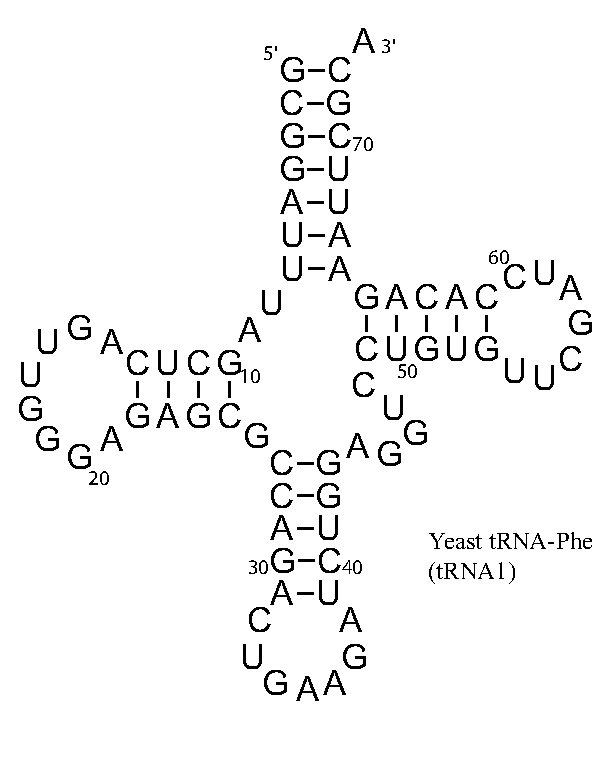
\includegraphics[scale=0.4]{Figures/trna1-DF6280}
\end{minipage}
\vspace{1em}

This is a simple example of a multiple RNA sequence alignment with
secondary structure annotation, in \emph{Stockholm format}.  Stockholm
format, the native alignment format used by HMMER and Infernal and the
Pfam and Rfam databases, is documented in detail later in the guide in
section~\ref{section:formats}.

For now, what you need to know about the key features of the input file is:
\begin{itemize}
\item The alignment is in an interleaved format.
Lines consist of a name, followed by an aligned sequence;
long alignments are split into blocks separated by blank lines.
\item Each sequence must have a unique name that has zero spaces in it. (This is important!)
\item For residues, any one-letter IUPAC nucleotide code is accepted,
      including ambiguous nucleotides. Case is ignored; residues
      may be either upper or lower case.
\item Gaps are indicated by the characters \otext{.}, \otext{\_}, -, or \verb+~+.
      (Blank space is not allowed.)
\item A special line starting with \otext{\#=GC SS\_cons} indicates
      the secondary structure consensus. Gap characters annotate
      unpaired (single-stranded) columns. Base pairs are indicated
      by any of the following pairs: \otext{<>}, \otext{()}, \otext{[]},
      or \otext{\{\}}. No pseudoknots are allowed; the
      open/close-brackets notation is only unambiguous for strictly
      nested base-pairing interactions.
      For more on secondary structure annotation see the WUSS format
      description in section~\ref{section:formats}.
\item The alignment begins with the special tag line
      \otext{\# STOCKHOLM 1.0}, and ends with \otext{//}.
      Stockholm alignments
      can be concatenated to create an alignment database flatfile
      containing many alignments.
\end{itemize}

The \prog{cmbuild} command builds a covariance model from an alignment (or
CMs for each of many alignments in a Stockholm file), and saves the
CM(s) in a file. For example, type:

\user{cmbuild tRNA5.cm tutorial/tRNA5.sto}

and you'll see some output that looks like:

\begin{sreoutput}
# cmbuild :: covariance model construction from multiple sequence alignments
# INFERNAL 1.1.4 (Dec 2020)
# Copyright (C) 2020 Howard Hughes Medical Institute.
# Freely distributed under the BSD open source license.
# - - - - - - - - - - - - - - - - - - - - - - - - - - - - - - - - - - - -
# CM file:                                            tRNA5.cm
# alignment file:                                     tutorial/tRNA5.sto
# - - - - - - - - - - - - - - - - - - - - - - - - - - - - - - - - - - - -
#                                                                      rel entropy
#                                                                      -----------
# idx    name                     nseq eff_nseq   alen  clen  bps bifs    CM   HMM description
# ------ -------------------- -------- -------- ------ ----- ---- ---- ----- ----- -----------
       1 tRNA5                       5     3.73     74    72   21    2 0.783 0.489 
#
# CPU time: 0.26u 0.00s 00:00:00.26 Elapsed: 00:00:00.27
\end{sreoutput}

If your input file had contained more than one alignment, you'd get
one line of output for each model. The information on these lines is
almost self-explanatory. The \otext{tRNA5} alignment consisted of 5
%  VERIFY WHEN UPDATING                                           ^
sequences with 74 aligned columns. Infernal turned it into a model of
%              ^^
72 consensus positions, which means it defined 2 gap-containing
%^                                             ^
alignment columns to be insertions relative to consensus. The 5
%                                                             ^
sequences were only counted as an ``effective'' total sequence number
(\otext{eff\_nseq}) of 3.73. The model includes 21 basepairs and 2
%                      ^^^^                     ^^               ^
bifurcations. The model ended up with a relative entropy per position
(\otext{rel entropy, CM}; information content) of 0.783 bits. If the
%                                                 ^^^^^
secondary structure information of the model were ignored the relative
entropy per position (\otext{rel entropy, HMM}) would be 0.489 bits.
%                                                        ^^^^^         
This output format is rudimentary. Infernal knows quite a bit more
information about what it's done to build this CM, but it's not
displaying it. You don't need to know more to be able to use the
model, so we can press on here. Model construction is described in
more detail in section~\ref{section:cmbuild}.

The new CM was saved to \otext{tRNA5.cm}. You can look at it
(e.g. \otext{> more tRNA5.cm}) if you like, but it isn't really designed
to be human-interpretable. You can treat \otext{.cm} files as compiled
models of your RNA alignment. The Infernal ASCII save file format is
defined in Section~\ref{section:formats}.

\subsubsection{Step 2: calibrate the model with cmcalibrate}

The next step is to ``calibrate'' the model. This step must be
performed prior to using your model for database searches with
\prog{cmsearch} or \prog{cmscan}. In this step, statistical parameters
necessary for reporting E-values (expectation values) are estimated
and stored in the CM file. When \prog{cmsearch} or \prog{cmscan} is
later used for a database search and a hit with score $x$ is found,
the E-value of that hit is the number of hits expected to score $x$ or
more just by chance (given the size of the search you're performing).

\emph{Importantly, if you're not going to use a model for database
search, there is no need to calibrate it.} For example, if you are
only going to use a model to create structurally annotated multiple
alignments of a large family like small subunit ribosomal RNA, don't
waste time calibrating it. \prog{cmsearch} and \prog{cmscan} are the
only Infernal programs that use E-values, so if you're not going to
use them then don't calibrate your model.

Unfortunately, CM calibration takes a long time because fairly long
random sequences must be searched to determine the expected
distribution of hit scores against nonhomologous sequences, and none
of the search acceleration heuristics described in
section~\ref{section:pipeline} can be used because they rely on
primary sequence similarity which is absent in random sequence.

The amount of time required for calibration varies widely, but
depends mainly on the size of the RNA family being modeled.
So you can know what kind of a wait you're in for, the
\prog{cmcalibrate} has a \otext{--forecast} option which reports an
estimate of the running time. To get an estimate for the tRNA model, do:

\user{cmcalibrate --forecast tRNA5.cm}\\

You should see something like this:

\begin{sreoutput}
# cmcalibrate :: fit exponential tails for CM E-values
# INFERNAL 1.1.4 (Dec 2020)
# Copyright (C) 2020 Howard Hughes Medical Institute.
# Freely distributed under the BSD open source license.
# - - - - - - - - - - - - - - - - - - - - - - - - - - - - - - - - - - - -
# CM file:                                     tRNA5.cm
# forecast mode (no calibration):              on
# - - - - - - - - - - - - - - - - - - - - - - - - - - - - - - - - - - - -
#
# Forecasting running time for CM calibration(s) on 32 cpus:
#
#                          predicted
#                       running time
# model name            (hr:min:sec)
# --------------------  ------------
  tRNA5                     00:00:58
#
# CPU time: 0.18u 0.01s 00:00:00.19 Elapsed: 00:00:00.18
[ok]
\end{sreoutput}

The header comes first, telling you what program you ran, on what file
and with what options. This calibration will use 32 CPUs, your output
%                                                ^^
may vary depending on how many cores you have available on the machine
you're using. (If you are planning to use MPI to parallelize the
calibration (see the Installation section), you can specify the number
of CPUs for the time estimate as \otext{<n>} with the
\otext{--nforecast <n>} option.) Using 32 CPUs, \prog{cmcalibrate}
estimates the time required for calibration on the machine I'm using
at about one minute.

Feel free to perform the calibration yourself if you'd like (with the
command \otext{cmcalibrate tRNA5.cm}). However, we've included the file
\otext{tRNA5.c.cm}, an already calibrated version of \otext{tRNA5.cm},
for you to use if you don't want to wait. To use this calibrated
model, copy over the \otext{tRNA5.cm} file you just made with the
calibrated version:
 
\user{cp tutorial/tRNA5.c.cm tRNA5.cm}\\
 
\subsubsection{Step 3: search a sequence database with cmsearch}

You can now use your tRNA model to search for tRNA homologs in a
database. The file \otext{mrum-genome.fa} is the genome sequence of the
archaeon \emph{Methanobrevibacter rumanitium} (accession:
\otext{NC\_13790.1}). We'll use this file as our database. To perform
the search:

\user{cmsearch tRNA5.cm tutorial/mrum-genome.fa}\\

As before, the first section is the header, telling you what program
your ran, on what, and with what options:

\begin{sreoutput}
# cmsearch :: search CM(s) against a sequence database
# INFERNAL 1.1.4 (Dec 2020)
# Copyright (C) 2020 Howard Hughes Medical Institute.
# Freely distributed under the BSD open source license.
# - - - - - - - - - - - - - - - - - - - - - - - - - - - - - - - - - - - -
# query CM file:                         tRNA5.cm
# target sequence database:              tutorial/mrum-genome.fa
# number of worker threads:              32
# - - - - - - - - - - - - - - - - - - - - - - - - - - - - - - - - - - - -
\end{sreoutput}

The second section is a list of ranked top hits (sorted by E-value,
most significant hit first):

\begin{sreoutput}
 rank     E-value  score  bias  sequence      start     end   mdl trunc   gc  description
 ----   --------- ------ -----  ----------- ------- -------   --- ----- ----  -----------
  (1) !   1.4e-18   71.4   0.0  NC_013790.1  362026  361955 -  cm    no 0.50  Methanobrevibacter ruminantium M1 chromosome, complete genome
  (2) !   3.3e-18   70.2   0.0  NC_013790.1 2585265 2585193 -  cm    no 0.60  Methanobrevibacter ruminantium M1 chromosome, complete genome
  (3) !   9.5e-18   68.7   0.0  NC_013790.1  762490  762562 +  cm    no 0.67  Methanobrevibacter ruminantium M1 chromosome, complete genome
  (4) !   9.5e-18   68.7   0.0  NC_013790.1 2041704 2041632 -  cm    no 0.67  Methanobrevibacter ruminantium M1 chromosome, complete genome
  (5) !   2.4e-17   67.5   0.0  NC_013790.1 2351254 2351181 -  cm    no 0.62  Methanobrevibacter ruminantium M1 chromosome, complete genome
  (6) !     3e-17   67.2   0.0  NC_013790.1  735136  735208 +  cm    no 0.59  Methanobrevibacter ruminantium M1 chromosome, complete genome
  (7) !   5.3e-17   66.4   0.0  NC_013790.1 2186013 2185941 -  cm    no 0.53  Methanobrevibacter ruminantium M1 chromosome, complete genome
  (8) !   1.7e-16   64.8   0.0  NC_013790.1 2350593 2350520 -  cm    no 0.66  Methanobrevibacter ruminantium M1 chromosome, complete genome
  (9) !   2.9e-16   64.1   0.0  NC_013790.1 2585187 2585114 -  cm    no 0.59  Methanobrevibacter ruminantium M1 chromosome, complete genome
 (10) !   9.3e-16   62.5   0.0  NC_013790.1  662185  662259 +  cm    no 0.61  Methanobrevibacter ruminantium M1 chromosome, complete genome
 (11) !   1.3e-15   62.0   0.0  NC_013790.1  360887  360815 -  cm    no 0.55  Methanobrevibacter ruminantium M1 chromosome, complete genome
 (12) !   1.7e-15   61.7   0.0  NC_013790.1 2350984 2350911 -  cm    no 0.53  Methanobrevibacter ruminantium M1 chromosome, complete genome
 (13) !   3.3e-15   60.7   0.0  NC_013790.1 2186090 2186019 -  cm    no 0.54  Methanobrevibacter ruminantium M1 chromosome, complete genome
 (14) !   4.3e-15   60.4   0.0  NC_013790.1 2680159 2680233 +  cm    no 0.67  Methanobrevibacter ruminantium M1 chromosome, complete genome
 (15) !   8.1e-15   59.5   0.0  NC_013790.1 2749839 2749768 -  cm    no 0.53  Methanobrevibacter ruminantium M1 chromosome, complete genome
 (16) !   8.1e-15   59.5   0.0  NC_013790.1 2749945 2749874 -  cm    no 0.53  Methanobrevibacter ruminantium M1 chromosome, complete genome
 (17) !     1e-14   59.2   0.0  NC_013790.1  361676  361604 -  cm    no 0.51  Methanobrevibacter ruminantium M1 chromosome, complete genome
 (18) !     1e-14   59.2   0.0  NC_013790.1 2585073 2584999 -  cm    no 0.60  Methanobrevibacter ruminantium M1 chromosome, complete genome
 (19) !   1.2e-14   59.0   0.0  NC_013790.1 2130422 2130349 -  cm    no 0.59  Methanobrevibacter ruminantium M1 chromosome, complete genome
 (20) !   1.3e-14   58.9   0.0  NC_013790.1  546056  545947 -  cm    no 0.61  Methanobrevibacter ruminantium M1 chromosome, complete genome
 (21) !   4.1e-14   57.3   0.0  NC_013790.1  361915  361844 -  cm    no 0.42  Methanobrevibacter ruminantium M1 chromosome, complete genome
 (22) !   5.2e-14   56.9   0.0  NC_013790.1   97724   97795 +  cm    no 0.49  Methanobrevibacter ruminantium M1 chromosome, complete genome
 (23) !   6.3e-14   56.7   0.0  NC_013790.1 2350717 2350646 -  cm    no 0.68  Methanobrevibacter ruminantium M1 chromosome, complete genome
 (24) !   8.3e-14   56.3   0.0  NC_013790.1 1873887 1873815 -  cm    no 0.64  Methanobrevibacter ruminantium M1 chromosome, complete genome
 (25) !   1.5e-13   55.5   0.0  NC_013790.1  360730  360659 -  cm    no 0.40  Methanobrevibacter ruminantium M1 chromosome, complete genome
 (26) !   3.6e-13   54.3   0.0  NC_013790.1 2680310 2680384 +  cm    no 0.52  Methanobrevibacter ruminantium M1 chromosome, complete genome
 (27) !   3.6e-13   54.3   0.0  NC_013790.1 2664806 2664732 -  cm    no 0.60  Methanobrevibacter ruminantium M1 chromosome, complete genome
 (28) !   3.8e-13   54.2   0.0  NC_013790.1  361061  360989 -  cm    no 0.41  Methanobrevibacter ruminantium M1 chromosome, complete genome
 (29) !   7.7e-13   53.3   0.0  NC_013790.1 2130335 2130262 -  cm    no 0.55  Methanobrevibacter ruminantium M1 chromosome, complete genome
 (30) !   7.7e-13   53.3   0.0  NC_013790.1 2151672 2151745 +  cm    no 0.65  Methanobrevibacter ruminantium M1 chromosome, complete genome
 (31) !   2.9e-12   51.4   0.0  NC_013790.1  319297  319370 +  cm    no 0.62  Methanobrevibacter ruminantium M1 chromosome, complete genome
 (32) !   3.9e-12   51.1   0.0  NC_013790.1  361753  361679 -  cm    no 0.55  Methanobrevibacter ruminantium M1 chromosome, complete genome
 (33) !     4e-12   51.0   0.0  NC_013790.1  360983  360912 -  cm    no 0.50  Methanobrevibacter ruminantium M1 chromosome, complete genome
 (34) !   6.1e-12   50.4   0.0  NC_013790.1  361456  361383 -  cm    no 0.50  Methanobrevibacter ruminantium M1 chromosome, complete genome
 (35) !   7.6e-12   50.1   0.0  NC_013790.1  362798  362727 -  cm    no 0.51  Methanobrevibacter ruminantium M1 chromosome, complete genome
 (36) !     9e-12   49.9   0.0  NC_013790.1  917722  917793 +  cm    no 0.61  Methanobrevibacter ruminantium M1 chromosome, complete genome
 (37) !     1e-11   49.7   0.0  NC_013790.1 2583869 2583798 -  cm    no 0.51  Methanobrevibacter ruminantium M1 chromosome, complete genome
 (38) !   1.4e-11   49.3   0.0  NC_013790.1  360811  360740 -  cm    no 0.42  Methanobrevibacter ruminantium M1 chromosome, complete genome
 (39) !   1.4e-11   49.3   0.0  NC_013790.1  362324  362252 -  cm    no 0.51  Methanobrevibacter ruminantium M1 chromosome, complete genome
 (40) !   4.3e-11   47.8   0.0  NC_013790.1 1160526 1160609 +  cm    no 0.60  Methanobrevibacter ruminantium M1 chromosome, complete genome
 (41) !     1e-10   46.6   0.0  NC_013790.1  362403  362331 -  cm    no 0.49  Methanobrevibacter ruminantium M1 chromosome, complete genome
 (42) !   1.1e-10   46.5   0.0  NC_013790.1 2327124 2327042 -  cm    no 0.63  Methanobrevibacter ruminantium M1 chromosome, complete genome
 (43) !   1.2e-10   46.4   0.0  NC_013790.1  995344  995263 -  cm    no 0.49  Methanobrevibacter ruminantium M1 chromosome, complete genome
 (44) !   2.3e-10   45.4   0.0  NC_013790.1  256772  256696 -  cm    no 0.57  Methanobrevibacter ruminantium M1 chromosome, complete genome
 (45) !   2.5e-10   45.3   0.0  NC_013790.1 2584830 2584758 -  cm    no 0.64  Methanobrevibacter ruminantium M1 chromosome, complete genome
 (46) !   6.3e-10   44.1   0.0  NC_013790.1 2351071 2350997 -  cm    no 0.59  Methanobrevibacter ruminantium M1 chromosome, complete genome
 (47) !   6.4e-10   44.1   0.0  NC_013790.1  362552  362482 -  cm    no 0.55  Methanobrevibacter ruminantium M1 chromosome, complete genome
 (48) !   5.1e-09   41.2   0.0  NC_013790.1 1064775 1064858 +  cm    no 0.63  Methanobrevibacter ruminantium M1 chromosome, complete genome
 (49) !   1.2e-08   40.0   0.0  NC_013790.1  361222  361150 -  cm    no 0.45  Methanobrevibacter ruminantium M1 chromosome, complete genome
 (50) !   1.3e-08   40.0   0.0  NC_013790.1  361369  361297 -  cm    no 0.60  Methanobrevibacter ruminantium M1 chromosome, complete genome
 (51) !   4.8e-08   38.1   0.0  NC_013790.1  361596  361513 -  cm    no 0.61  Methanobrevibacter ruminantium M1 chromosome, complete genome
 (52) !   3.1e-07   35.6   0.0  NC_013790.1 1913310 1913227 -  cm    no 0.64  Methanobrevibacter ruminantium M1 chromosome, complete genome
 (53) !   2.6e-06   32.7   0.0  NC_013790.1  363464  363381 -  cm    no 0.51  Methanobrevibacter ruminantium M1 chromosome, complete genome
 (54) !     3e-06   32.5   0.0  NC_013790.1 2584954 2584872 -  cm    no 0.58  Methanobrevibacter ruminantium M1 chromosome, complete genome
 ------ inclusion threshold ------
 (55) ?     0.026   20.1   0.0  NC_013790.1  363803  363716 -  cm    no 0.50  Methanobrevibacter ruminantium M1 chromosome, complete genome
 (56) ?       3.4   13.4   0.0  NC_013790.1  984373  984304 -  cm    no 0.53  Methanobrevibacter ruminantium M1 chromosome, complete genome
\end{sreoutput}

The first number is the rank of each hit\footnote{Ranks of hits are in
  parantheses to make it easy to jump to/from an entry in the hit list
  and the hit alignment section, described later.}. Next comes either a
\otext{!} or \otext{?} symbol and then the \emph{E-value} of the hit.
The E-value is the statistical significance of the hit: the number of
hits we'd expect to score this highly in a database of this size
(measured by the total number of nucleotides) if the database
contained only nonhomologous random sequences. The lower the E-value,
the more significant the hit. The \otext{!} or \otext{?} that
precedes the E-value indicates whether the hit does (\otext{!}) or
does not (\otext{?}) satisfy the inclusion threshold for the search.
Inclusion thresholds are used to determine what matches should be
considered to be ``true'', as opposed to reporting thresholds that
determine what matches will be reported (often including the top of
the noise, so you can see what interesting sequences might be getting
tickled by your search). By default, inclusion thresholds usually
require an E-value of 0.01 or less, and reporting E-value thresholds
are set to 10.0, but these can be changed (see the manual page for
\prog{cmsearch} toward the end of guide).

The E-value is based on the \emph{bit score}, which is in the next
column. This is the log-odds score for the hit. Some people like to
see a bit score instead of an E-value, because the bit score doesn't
depend on the size of the sequence database, only on the covariance
model and the target sequence.

The next number, the \emph{bias}, is a correction term for biased
sequence composition that has been applied to the sequence bit
score. Infernal uses an alternative null model we call \emph{null3},
described more in section~\ref{section:pipeline}, to determine the bias
bit score correction. The bias correction is often very small and is
only reported to one decimal place, after rounding. For all hits in
this example search the bias column reads 0.0 bits, indicating that
the correction is less than 0.05 bits. On very biased sequences this
correction can become significant and is helpful for lowering the
score of high-scoring false positives that achieve high scores solely
due to their biased composition. 

Next comes the target sequence name the hit is in, and the start and
end positions of the hit within the sequence. Hits can occur on either
the top (Watson) or bottom (Crick) strand of the target
sequence\footnote{You can search either only the top strand with the
\otext{--toponly} or bottom strand with the \otext{--bottomonly} options
to \prog{cmsearch} and \prog{cmscan}.}, so the start position may be
less than (if hit is on the top strand) or greater than (if hit is on
the bottom strand) the end position. After the end position, comes a single
\otext{+} or \otext{-} symbol, indicating whether the hit is on the
top (\otext{+}) or bottom (\otext{-}) strand (solely for convenience -
so you don't have to look at the start and end positions to determine
the strand the hit is on).

After the strand symbol comes the model field, which indicates whether
the hit was found using either the CM (\otext{cm}) or a profile HMM
built from the CM (\otext{hmm}). This field is necessary because for
models with zero basepairs, \prog{cmsearch} (and \prog{cmscan}) use a
profile HMM instead of a CM for final hit scoring. This is done for
reasons of speed and efficiency, because profile HMM algorithms are
more efficient than CM ones and a CM with zero basepairs is
essentially equivalent to a profile HMM. In this example, since our
tRNA model does include basepairs, \prog{cmsearch} used a CM to score
all hits and so all hits have \prog{cm} for this column. There's an
example later in the tutorial of hits found with a profile HMM.

The next column indicates whether the hit is \emph{truncated} or
not. Infernal uses special versions of its CM dynamic programming
algorithms to allow detection of structural RNAs that have been
truncated due to missing data at the beginning and/or end of a target
sequence. Truncated hits are most common in databases that include
single reads from shotgun sequencing projects. Since our database is a
complete genome, we don't expect any hits to be truncated due to
missing data. For all hits the ``trunc'' column reads
``no'' indicating that, as expected, none of the hits are
truncated. There are examples of truncated hits in the next exercise
which uses \prog{cmscan}. Section~\ref{section:pipeline} describes how
Infernal detects and aligns truncated hits in more detail.

The next column reports the GC fraction of the hit. This is the
fraction of residues in the target sequence hit that are either G or C
residues. The GC fraction is included as an additional indication of
the level of sequence bias of the hit. Some expert users may be aided
by this number when deciding if they believe a hit is a real homolog
or a false positive.

Finally comes the description of the sequence, if any. This
description is propogated from the input target sequence file.

After the hit list comes the hit alignments section. Each hit in 
the hit list will have a corresponding entry in this section, in the
same order. As an illustrative example, let's take a look at
hit number 43. First, take a look at the first four lines for this
hit: 

\begin{sreoutput}
>> NC_013790.1  Methanobrevibacter ruminantium M1 chromosome, complete genome
 rank     E-value  score  bias mdl mdl from   mdl to       seq from      seq to       acc trunc   gc
 ----   --------- ------ ----- --- -------- --------    ----------- -----------      ---- ----- ----
 (43) !   1.2e-10   46.4   0.0  cm        1       72 []      995344      995263 - .. 0.93    no 0.49
\end{sreoutput}

The first line of each hit alignment begins with \otext{>>} followed
by a single space, the name of the target sequence, then two spaces
and the description of the sequence, if any. Next comes a set of
tabular fields that is partially redundant with the information in the
hit list. The first five columns are the same as in the hit list. The
next column reports the type of model used for the alignment, as
described above for the hit list. The next four columns report the
boundaries of the alignment with respect to the query model (``mdl
from'' and ``mdl to'') and the target sequence (``seq from'' and ``seq
to''). Following the ``seq to'' column is a \otext{+} or \otext{-}
symbol indicating whether the hit is on the top (\otext{+}) or bottom
(\otext{-}) strand.

It's not immediately easy to tell from the ``to'' coordinate whether
the alignment ended internally in the query model or target sequence,
versus ran all the way (as in a full-length global alignment) to the
end(s). To make this more readily apparent, with each pair of query
and target endpoint coordinates, there's also a little symbology. For
the normal case of a non-truncated hit: \otext{..} means both ends of
the alignment ended internally, and \otext{[]} means both ends of the
alignment were full-length flush to the ends of the query or target,
and \otext{[.}  and \otext{.]} mean only the left (5') or right (3') end
was flush/full length. For truncated hits, the symbols are the same
except that either the first and/or the second symbol will be a
\verb+~+ for the query and target. If the first symbol is \verb+~+
then the left end of the alignment is truncated because the 5' end of
the hit is predicted to be missing (extend beyond the beginning of the
target sequence). Similarly, if the second symbol is \verb+~+ then the
right end of the alignment is truncated because the 3' end of the hit
is predicted to be missing (extend beyond the end of the target
sequence). These two symbols occur just after the ``mdl to'' column for
the query, and after the strand \otext{+} or \otext{-} symbol for the
target sequence.

The next column is labeled ``acc'' and is the average posterior
probability of the aligned target sequence residues; effectively, the
expected accuracy per residue of the alignment. (This field may be
absent and replaced by a column labeled ``cyksc'' in certain
situations, as explained more below.)

The final two columns indicate whether the hit is truncated or not and
the GC fraction of the hit. These are redundant with the columns of
the same name in the hit list, described above.

Next comes the alignment display. This is an ``optimal
posterior accuracy'' alignment~\citep{Holmes98}, which means it is the
alignment with the maximal summed posterior probability of all
aligned residues. Take a look at the alignment for hit number 43:

\begin{sreoutput}
                                 v         v                                                            NC
                     (((((((,,<<<<______.._>>>>,<<<<<_______>>>>>,,,........,,<<<<<_______>>>>>))))))): CS
        tRNA5      1 gCcggcAUAGcgcAgUGGu..AgcgCgccagccUgucAagcuggAGg........UCCgggGUUCGAUUCcccGUgccgGca 72    
                     :::G:CAUAGCG AG GGU  A CGCG:CAG:CU +++A:CUG: G+        UC:GGGGUUCGA UCCCC:UG:C:::A
  NC_013790.1 995344 AGAGACAUAGCGAAGCGGUcaAACGCGGCAGACUCAAGAUCUGUUGAuuaguucuUCAGGGGUUCGAAUCCCCUUGUCUCUA 995263
                     **********************************************9444444445************************** PP
\end{sreoutput}

The alignment contains six lines. Start by looking at the second line
which ends with \otext{CS}.  The line shows the predicted secondary
structure of the target sequence. The format is a little fancier and
more informative than the simple least-common-denominator format we
used in the input alignment file. It's designed to make it easier to
see the secondary structure by eye. The format is described in detail
later (see WUSS format in section~\ref{section:formats}); for now,
here's all you need to know. Basepairs in simple stem loops are
annotated with \otext{<>} characters. Basepairs enclosing
multifurcations (multiple stem loops) are annotated with \otext{()},
such as the tRNA acceptor stem in this example. In more complicated
structures, \otext{[]} and \otext{\{\}} annotations also show up, to
reflect deeper nestings of multifurcations. For single stranded
residues, \otext{\_} characters mark hairpin loops; \otext{-}
characters mark interior loops and bulges; \otext{,} characters mark
single-stranded residues in multifurcation loops; and \otext{:}
characters mark single stranded residues external to any secondary
structure. Insertions relative to this consensus are annotated by a
\otext{.} character.

The line above the \otext{CS} line ends with \otext{NC} and marks
negative scoring non-canonical basepairs in the alignment with a
\otext{v} character. All other positions of the alignment will be
blank\footnote{For anyone trying to parse this output, this means it
is possible for this line to be completely blank except for the
\otext{NC} trailer.} More specifically, the following ten types of
basepairs which are assigned a negative score by the model at their
alignment positions will be marked with a \otext{v}: \otext{A:A},
\otext{A:C}, \otext{A:G}, \otext{C:A}, \otext{C:C}, \otext{C:U},
\otext{G:A}, \otext{G:G}, \otext{U:U}, and \otext{U:C}. The \otext{NC}
annotation makes it easy to quickly identify suspicious basepairs in
a hit. Importantly, the \otext{NC} annotation will only be present in
CM hit alignments (``mdl'' column reads ``cm'') and will be absent in
HMM hit alignments (``mdl'' column reads ``hmm'') because basepairs
are not scored by an HMM.

The third line shows that consensus of the query model. The highest
scoring residue sequence is shown. Upper case residues are highly
conserved. Lower case residues are weakly conserved or unconserved.
Dots (\otext{.}) in this line indicate insertions in the target
sequence with respect to the model.

The fourth line shows where the alignment score is coming from. For a
consensus basepair, if the observed pair is the highest-scoring
possible pair according to the consensus, both residues are shown in
upper case; if a pair has a score of $\geq 0$, both residues are
annotated by : characters (indicating an acceptable compensatory
basepair); else, there is a space, indicating that a negative
contribution of this pair to the alignment score. Note that the 
\otext{NC} line will only mark a subset of these negative scoring
pairs with a \otext{v}, as discussed above.
For a single-stranded consensus residue, if the observed residue is
the highest scoring possibility, the residue is shown in upper case;
if the observed residue has a score of $\geq 0$, a \otext{+} character
is shown; else there is a space, indicating a negative contribution to
the alignment score. Importantly, for HMM hits (``mdl'' column reads
``hmm''), \emph{all} positions are considered single stranded, since
an HMM scores each half of a basepair independently.

The fifth line, beginning with \otext{NC\_013790.1} is
the target sequence. Dashes (\otext{-}) in this line indicate deletions
in the target sequence with respect to the model.

The bottom line represents the posterior probability (essentially the
expected accuracy) of each aligned residue. A 0 means 0-5\%, 1 means
5-15\%, and so on; 9 means 85-95\%, and a \otext{*} means 95-100\%
posterior probability. You can use these posterior probabilities to
decide which parts of the alignment are well-determined or not. You'll
often observe, for example, that expected alignment accuracy degrades
around locations of insertion and deletion, which you'd intuitively
expect.

Alignments for some searches may be formatted slightly differently
than this example. Longer alignments to longer models will be broken
up into blocks of six lines each - this alignment was short enough to
be entirely contained within a single block.  If your model was built
with the \otext{--hand} option in \prog{cmbuild}, then an additional
line will be included in each block, with RF annotation.  If the model
used for the alignment was an HMM (the ``mdl'' column reads ``hmm'')
then the \otext{NC} line will be absent from each alignment
block. We'll see example of all three of these cases later in the
tutorial. Finally, the \otext{PP} line will be absent if
\prog{cmsearch} has determined that calculating posterior
probabilities for the optimal posterior accuracy alignment would have
required more than a preset amount of memory (that amount is
autodetermined based on model size, but is capped at a maximum of
512Mb for the largest models, unless the \emprog{--mxsize} option is
used to increase it). If the \otext{PP} line is absent, the tabular
``acc'' field described above will be absent and replaced with a
``cyksc'' field which reports the bit score of the highest scoring CYK
alignment, and the displayed alignment will be the alignment computed
by the CYK algorithm which requires less memory than the ``optimal
posterior accuracy'' alignment.

After hit number 43, there's 13 more hit alignments for hits number 44
through 56. 

Finally, at the bottom of the file, you'll see some summary
statistics. For example, at the bottom of the tRNA search output,
you'll find something like:

\newpage

\begin{sreoutput}
Internal CM pipeline statistics summary:
----------------------------------------
Query model(s):                                                  1  (72 consensus positions)
Target sequences:                                                1  (5874406 residues searched)
Target sequences re-searched for truncated hits:                 1  (360 residues re-searched)
Windows   passing  local HMM SSV           filter:           10932  (0.2063); expected (0.35)
Windows   passing  local HMM Viterbi       filter:                  (off)
Windows   passing  local HMM Viterbi  bias filter:                  (off)
Windows   passing  local HMM Forward       filter:             136  (0.002704); expected (0.005)
Windows   passing  local HMM Forward  bias filter:             133  (0.002634); expected (0.005)
Windows   passing glocal HMM Forward       filter:              84  (0.001948); expected (0.005)
Windows   passing glocal HMM Forward  bias filter:              84  (0.001948); expected (0.005)
Envelopes passing glocal HMM envelope defn filter:              99  (0.001331); expected (0.005)
Envelopes passing  local CM  CYK           filter:              60  (0.0007629); expected (0.0001)
Total CM hits reported:                                         56  (0.0007205); includes 0 truncated hit(s)

# CPU time: 1.91u 0.09s 00:00:02.00 Elapsed: 00:00:01.09
//
[ok]
\end{sreoutput}

This gives you some idea of what's going on in Infernal's acceleration
pipeline. You've got one query CM, and the database has one target
%                    ^                                  ^
sequence. The search examined 5,874,406 residues, even though the
%                             ^^^^^^^^^
actual target sequence length is only half that, because both the top
and bottom strand of each target is searched. 360 of those residues
%                                             ^^^
were searched more than once in an effort to find truncated
hits. Ignore this for the moment, we'll revisit this later after
discussing the filter pipeline (in the subsection entitled ``Truncated
RNA detection'' below).

Each sequence goes through a multi-stage filter pipeline of four
scoring algorithms called SSV, Viterbi, Forward\footnote{Actually two
  separate Forward based filters are used, the first with the profile
  HMM in local mode and the next with the profile HMM in global
  mode. There's more detail on this in
  section~\ref{section:pipeline}.}, and CYK in order of increasing
sensitivity and increasing computational requirement. The filter
pipeline is the topic of section~\ref{section:pipeline} of this guide
but briefly, SSV, Viterbi and Forward are profile HMM algorithms which
are more efficient than CM algorithms. These three algorithms are the
same ones used by HMMER3 and are the main reason that version 1.1 of
Infernal is so much faster than previous versions. For these HMM
stages, Infernal uses a filter profile HMM that was constructed
simultaneously with the CM, from the same training alignment in
\prog{cmbuild}, and stored in the CM file. CYK is a CM scoring
algorithm, so it's slow, but it is accelerated using banded dynamic
programming with bands derived from an HMM alignment. Subsequences
that survive all filters are finally scored with the CM Inside
algorithm, agains using HMM bands. Subsequences that score
sufficiently high with Inside are then aligned using the optimal
posterior accuracy algorithm and displayed.

The score thresholds for a subsequence surviving each HMM filter stage
are dependent on the search space size (sequence database size for
\prog{cmsearch}). This differs from HMMER3 which always uses the same
filter thresholds. In general, the larger the search
space the more strict the thresholds are, because a hit must have a
higher bit score to have a significant E-value.  In this case, the
database is relatively small so the filter thresholds have been set
relatively loosely. The SSV filter has been configured to allow
subsequences with a P-value of $\leq 0.35$ through
%                                   ^^^^^^
the SSV score filter (thus, if the database contained no homologs and
P-values were accurately calculated, the highest scoring 35\% of the
%                                           ^^^^
residues will pass the filter). Here, about 21\% of the database in
%                                           ^^^^
10,932 separate windows got through the SSV filter. For a database of
%^^^^^
this size, the local Viterbi filter is turned off.  The local Forward filter
is set to allow an expected 0.5\% of the database survive. Here about
%                           ^^^^
0.3\% survives in 136 windows. Next, each surviving window is checked
%^^
to see if the target sequence is ``obviously'' so biased in its
composition that it's unlikely to be a true homolog. This is called
the ``bias filter''\footnote{There's also a bias filter step used in
  the local Viterbi filter stage, when it is used.} and applying a bit
score correction to previous filter's score for each window and
recomputing the P-value. Three of the 136 windows fail to pass
%                        ^^^^^        ^^^
the local Forward bias filter stage. Next, the Forward algorithm is
used to score each window again, but this time with the HMM configured
in glocal mode requiring a full length alignment to the
model\footnote{The use of glocal Forward is another important
  difference between Infernal and HMMER3's (v3.0) pipeline. HMMER v3.0
  only uses local HMM algorithms.}  As with the local stage, an
expected 0.5\% of the database is expected to survive. In this case,
84 of the 134 windows, comprising about 0.2\% of the database,
%^        ^^^
survive. The bias filter is run again, this time applying a correction
to the glocal Forward scores. For this search, 0 windows are removed at
this stage. The envelope definition stage is next. This stage is very
similar to the HMMER3 domain definition stage, with the difference
that the HMM is configured in glocal rather than local mode. In this
stage, the Forward and Backward algorithms are used to identify zero
or more hit envelopes in each window, where each envelope contains one
putative hit.  Often residues at the beginning and ends of windows are
determined to be nonhomologous and are not included in the
envelope. In this search,  99 envelopes are defined within the 84
%                         ^^^                                  ^^
windows. Note that the envelopes comprise only about 70\% of the
%                                                    ^^^
residues from the 84 windows, indicated by the drop of 0.1948\% to
%                                                      ^^^^^^^^
0.1331\%.
%%^^^^

After hit envelopes have been defined with the filter HMM, the two
remaining stages of the pipeline use the CM to score both the
conserved sequence and structure of each possible hit. In both of
these stages, constraints are derived from an HMM alignment of the
envelope and enforced as \emph{bands} on the CM dynamic programming
matrices (more on this in section~\ref{section:pipeline}). In the
first CM stage, the CYK algorithm (which is the SCFG analog of the
Viterbi HMM algorithm) is used to determine the best scoring maximum
likelihood alignment of any subsequence in each envelope to the CM. If
this alignment has a P-value of $\leq 0.0001$ then the envelope
survives to the final round. The envelopes passed to the final stage
may be shorter than those examined during the CYK stage. Specifically,
envelopes are redefined as starting and ending at the first and final
residues for which at least one alignment exists with a P-value $\leq
0.001$.

In the final round, the Inside algorithm (the SCFG analog of the HMM
Forward algorithm) is used to define final hit boundaries and
scores. Hits with scores above the reporting threshold were output, as
described above. In this search there were 56 such hits.
%                                          ^^

Finally, the running time of the search is reported, in CPU time and
elapsed time. This search took about 1 second (wall
clock time) running on 32 cores. 
%                      ^^^^^^^^^^^
\subsubsection{Truncated RNA detection}

Now, we come back to the topic of truncated hit detection.  As briefly
mentioned above, the pipeline statistics summary from our search above
reported that 360 residues were re-searched for truncated
%             ^^^
hits. Infernal explicitly looks at the 5' and 3' ends of target
sequences using specialized algorithms for detection of truncated
hits, in which part of the 5' and/or 3' end of the actual full length
sequence from the source organism's full genomic context is missing in
the input target sequence. Truncated hits will be most common in
sequence files consisting of unassembled sequencing reads. In our
search of the full archaeal genome above, no truncated hits were
found. However, there is an example of a truncated hit in the
\prog{cmscan} tutorial section below in a sequence from a metagenomics
sequencing survey.

Special dynamic programming algorithms are required for truncated hit
detection \citep{KolbeEddy09}, so sequences must be re-searched for
truncated hits after they are initially searched for standard
(non-truncated) hits. However, only the sequence ends must be
re-searched because Infernal assumes that only hits at sequence
terminii might be truncated. This is why our search above reported
that only 360 residues were re-searched for truncated hits. For each
%         ^^^
model, an expected maximum length of a hit\footnote{The expected
  maximum hit length is defined as the maximum of 1.25 times the
  consensus length of the model and the $W$ parameter computed with
  the QDB algorithm \citep{NawrockiEddy07}. $W$ is computed based on
  the transition probabilities of the model by \prog{cmbuild} and
  stored in the CM file.} 
is used to define the window length at the
beginning and end of each sequence which must be re-searched for
truncated hits. For our tRNA model the maximum expected length is
90, so exactly 360 residues were re-searched: the first and final 90
%^             ^^^                                                ^^
residues on the top strand, and the first and final 90 residues on
%                                                   ^^
the bottom strand.

There is one more aspect of truncated hit detection that is important
to mention here. Because Infernal expects that hit truncation only
occurs at the ends of sequences, 5' truncated hits are forced to start
at the first nucleotide of a sequence, 3' truncated hits are forced to
end at the final nucleotide of the sequence, and 5' \emph{and} 3'
truncated hits are forced to include the full sequence.

The annotation of truncated hits in \prog{cmsearch} output is slightly
different than for standard (non-truncated) hits. An example is
included in the next section below.

\subsection{Searching a CM database with a query sequence}

The \prog{cmscan} program is for annotating all the different
known/detectable RNAs in a given sequence. It takes a single query
sequence and a CM database as input. The CM database might be Rfam,
for example, or another collection of your choice. \prog{cmscan} is
new to version 1.1 of Infernal. It is designed to be useful for
sequence datasets from RNA-Seq experiments or metagenomics surveys,
for which one wants to know what families of RNAs are represented in
the sequence dataset.

\subsubsection{Step 1: create an CM database flatfile}

A CM ``database'' flatfile is simply a concatenation of individual CM
files. To create a database flatfile, you can either build and
calibrate individual CM files and concatenate them, or you can
concatenate Stockholm alignments and use \prog{cmbuild} to build a CM
database of all of them in one command, and then calibrate that
database with \prog{cmcalibrate}. Importantly, \prog{cmscan} can only
be used with calibrated CMs.

Let's create a tiny database called \otext{minifam.cm} containing the
tRNA model we've been working with, a 5S ribosomal RNA model, and a
Cobalamin riboswitch model. To save you time, calibrated versions of
the 5S and Cobalamin models are included in the \otext{tutorial/}
directory in the files \otext{5S\_rRNA.c.cm}, and
\otext{Cobalamin.c.cm}. These files were created using \prog{cmbuild}
and \prog{cmcalibrate} from the Rfam 10.1 seed alignments for 5S\_rRNA
(RF00001) and Cobalamin (RF00174), provided in
\otext{tutorial/5S\_rRNA.sto} and \otext{tutorial/Cobalamin.sto}. The
third model is the tRNA model from earlier in the tutorial 
(\otext{tRNA5.c.cm}). Feel free to build and calibrate these
models yourself if you'd like, but if you'd like to keep moving on
with the tutorial, use the pre-calibrated ones. To create the database,
simply concatenate the three provided files:

\user{cat tutorial/tRNA5.c.cm tutorial/5S\_rRNA.c.cm tutorial/Cobalamin.c.cm > minifam.cm}

\subsubsection{Step 2: compress and index the flatfile with cmpress}

The \prog{cmscan} program has to read a lot of CMs and their filter
HMMs in a hurry, and Infernal's ASCII flatfiles are bulky. To
accelerate this, \prog{cmscan} uses binary compression and indexing of
the flatfiles. To use \prog{cmscan}, you must first compress and
index your CM database with the \prog{cmpress} program:

\user{cmpress minifam.cm}

This will quickly produce:

\begin{sreoutput}
Working...    done.
Pressed and indexed 3 CMs and p7 HMM filters (3 names and 2 accessions).
Covariance models and p7 filters pressed into binary file:  minifam.cm.i1m
SSI index for binary covariance model file:                 minifam.cm.i1i
Optimized p7 filter profiles (MSV part)  pressed into:      minifam.cm.i1f
Optimized p7 filter profiles (remainder) pressed into:      minifam.cm.i1p
\end{sreoutput}

and you'll see these four new binary files in the directory. 

The \otext{tutorial} directory includes a copy of the
\otext{minifam.cm} file, which has already been pressed, so there
are example binary files \otext{tutorial/minifam.cm.i1\{m,i,f,p\}}
included in the tutorial.

Their format is ``proprietary'', which is an open source term of art
that means both ``We haven't found time to document them yet'' and ``We
still might decide to change them arbitrarily without telling you''.

\subsubsection{Step 3: search the CM database with cmscan}

Now we can analyze sequences using our CM database and
\prog{cmscan}. 

For example, the file \otext{tutorial/metag-example.fa} includes 3
sequences (whole genome shotgun sequencing reads) derived from samples
of ``whale fall'' carcasses in a metagenomics study
\citep{Tringe05}. These three sequences were chosen from the roughly
200,000 in the complete dataset because they include statistically
significant hits to the three models in our toy CM database.

To scan the sequences with our database: 

\user{cmscan minifam.cm tutorial/metag-example.fa}

The header and the first section of the output will look like:

\begin{sreoutput}
# cmscan :: search sequence(s) against a CM database
# INFERNAL 1.1.4 (Dec 2020)
# Copyright (C) 2020 Howard Hughes Medical Institute.
# Freely distributed under the BSD open source license.
# - - - - - - - - - - - - - - - - - - - - - - - - - - - - - - - - - - - -
# query sequence file:                   tutorial/metag-example.fa
# target CM database:                    minifam.cm
# number of worker threads:              32
# - - - - - - - - - - - - - - - - - - - - - - - - - - - - - - - - - - - -

Query:       AAGA01015927.1  [L=943]
Description: Metagenome sequence AHAI1002.g1, whole genome shotgun sequence
Hit scores:
 rank     E-value  score  bias  modelname  start    end   mdl trunc   gc  description
 ----   --------- ------ -----  --------- ------ ------   --- ----- ----  -----------
  (1) !   1.5e-23   92.7   0.0  5S_rRNA       59    174 +  cm    no 0.66  5S ribosomal RNA
  (2) !   9.6e-19   62.4   0.0  tRNA5        229    302 +  cm    no 0.62  -
  (3) !   6.1e-16   53.5   0.0  tRNA5        314    386 +  cm    no 0.59  -
\end{sreoutput}

\prog{cmscan} has identified three putative RNAs in the first query
sequence, one 5S rRNA and two tRNAs. The output fields are in the
same order and have the same meaning as in \prog{cmsearch}'s output.

Before we move on, this is a good opportunity to point out an
important difference between \prog{cmsearch} and \prog{cmscan} related
to the size of the search space (often referred to in the code and in
this guide as the $Z$ parameter).  The size of the search space for
\prog{cmscan} is double the length of the current (single) query
sequence (doubled because we're searching both strands) multiplied by
the number of models in the CM database (here, 3; for a Rfam search,
on the order of 1000). Because each query sequence is probably a
different size this means $Z$ changes for each query sequence. In
\prog{cmsearch}, the size of the search space is double the summed
length of all sequences in the database (again, doubled because both
strands are searched). This means that E-values may differ even for
the same individual CM vs. sequence comparison, depending on how you
do the search. The search space size also affects what filter
thresholds \prog{cmsearch} or \prog{cmscan} will use, which is
discussed more in section~\ref{section:pipeline}.

Now back to the \prog{cmscan} results. What follows the ranked list of
three hits are the hit alignments. These are constructed and annotated
the same as in \prog{cmsearch}. The 5S alignment is:

\begin{widesreoutput}
                             v               v       v         v         v             v            v                NC
                     (((((((((,,,,<<-<<<<<---<<--<<<<<<_______>>-->>>>-->>---->>>>>-->><<<-<<----<-<<-----<<____>>-- CS
         5S_rRNA   1 ccuggcggcCAUAgcggggcggAaacACccGauCCCAUCCCGaACuCggAAguUAAGcgcccuagcgccgggguAGuAcuggGgUGgGuGAcCaC 95 
                     CCUGGC:G C UAGCG:GG:GG   CACC:GA CCCAU CCG ACUC:GAAG  AA+C:CC:UAGC CCG::G  G:A: G+G  GGGU  CC C
  AAGA01015927.1  59 CCUGGCGGCCGUAGCGCGGUGGUCCCACCUGACCCCAUGCCGAACUCAGAAGUGAAACGCCGUAGCGCCGAUG--GUAGUGUG--GGGUCUCCCC 149
                     *************************************************************************..********..********** PP

                        v         v v          NC
                     --->>->->>->>>,))))))))): CS
         5S_rRNA  96 cUGggAaaccagguCgccgccaggc 120
                      UG :A:A::AGG   C:GCCAGGC
  AAGA01015927.1 150 AUGCGAGAGUAGGGAACUGCCAGGC 174
                     ************************* PP
\end{widesreoutput}

After the three sequences, you'll see a pipeline statistics summary
report:

\newpage

\begin{widesreoutput}
Internal CM pipeline statistics summary:
----------------------------------------
Query sequence(s):                                               1  (1886 residues searched)
Query sequences re-searched for truncated hits:                  1  (834.7 residues re-searched, avg per model)
Target model(s):                                                 3  (382 consensus positions)
Windows   passing  local HMM SSV           filter:              20  (0.3992); expected (0.35)
Windows   passing  local HMM Viterbi       filter:                  (off)
Windows   passing  local HMM Viterbi  bias filter:                  (off)
Windows   passing  local HMM Forward       filter:               4  (0.07976); expected (0.02)
Windows   passing  local HMM Forward  bias filter:               4  (0.07976); expected (0.02)
Windows   passing glocal HMM Forward       filter:               2  (0.06641); expected (0.02)
Windows   passing glocal HMM Forward  bias filter:               2  (0.06641); expected (0.02)
Envelopes passing glocal HMM envelope defn filter:               3  (0.03357); expected (0.02)
Envelopes passing  local CM  CYK           filter:               3  (0.03357); expected (0.0001)
Total CM hits reported:                                          3  (0.03222); includes 0 truncated hit(s)

# CPU time: 0.06u 0.03s 00:00:00.09 Elapsed: 00:00:00.05
//
\end{widesreoutput}

This report is similar to the one you saw earlier from
\prog{cmsearch}, but not identical. One big difference is that
\prog{cmscan} will report a summary per query sequence, instead of per
query model. In this case, the sequence was 943 residues long, so a
%                                           ^^^
total of 1886 residues were searched, since both strands were
%        ^^^^
examined. The next line reports that the average number of residues
re-searched for truncated hits per model was 834.7. An average is
%                                            ^^^^^
reported here because remember the number of residues re-searched per
model depends on the expected maximum size of a hit, which varies per
model, because only sequence terminii are examined for truncated hits
(see ``Truncated RNA detection'' above and
section~\ref{section:pipeline}).  The remainder of the output is the
same as in \prog{cmsearch} except that the fractional values are
averages per model. For example, for all three models a total of 3
envelopes survived the CYK filter stage, and those surviving envelopes
contained 3.357\% of the target sequence \emph{on average per model}.
%         ^^^^^

You may have noticed that the expected survival fractions are
different than they were in the \prog{cmsearch} example. This is
because the P-value filter thresholds are set differently depending on
the search space. For this example, the search space ($Z$) is roughly
only 6 Kb (1886 residues in the query sequence multiplied by 3 target
models), so the thresholds are set differently than for the
\prog{cmsearch} example which had a search space size of roughly 6
Mb. The exact thresholds used for various $Z$ values can be found in
Table~\ref{tbl:thresholds} in section~\ref{section:pipeline}.

\subsubsection{Truncated hit and local end alignment example}
Next, take a look at the \prog{cmscan} output for the second query
sequence \otext{AAFY01022046.1}. The bottom strand of this sequence
contains one hit to the Cobalamin riboswitch model, which is truncated
at the 5' end. Here is the alignment:

\begin{widesreoutput}
Hit alignments:
>> Cobalamin  Cobalamin riboswitch
 rank     E-value  score  bias mdl mdl from   mdl to       seq from      seq to       acc trunc   gc
 ----   --------- ------ ----- --- -------- --------    ----------- -----------      ---- ----- ----
  (1) !   6.6e-09   29.9   0.0  cm       31      190 ~]         934         832 - ~. 0.92    5' 0.48

                                 ???              v           v      v    v                                     ???? NC
                     ~~~~~~______>>>,,,,,(((,,,<.<<<<_______>>>>>,,<<<____>>>,<<<---<<<<~~~~~~>>>>---->>>,,,,)))]]]] CS
       Cobalamin   1 <[30]*agucggggguuAAaaGGGAAc.ccGGUGcaAauCCgggGCuGcCCCCgCaACUGUAAgcGg*[61]*cCgcgAGCCAGGAGACCuGCCg 173
                           + + G     + AA: GGAA: : GGUG AAAUCC ::+C:G CCC  C:ACUGUAA:C:        :G:+AG+CAG A AC :  C 
  AAFY01022046.1 934 <[ 0]*GUAGGCAAAAGGAAGAGGAAGgAUGGUGGAAAUCCUUCACGGGCCCGGCCACUGUAACCAG*[ 4]*UUGGAAGUCAG-AUACUCUUCU 849
                     ......44455677788899******9899***********************************96...7..69*********.9********* PP

                     ??                NC
                     ]]::::::::::::::: CS
       Cobalamin 174 ucaaaaauaguaucacc 190
                       +AA +  G+A+C+ C
  AAFY01022046.1 848 AUUAAGGCGGAAACUAC 832
                     ***************** PP
\end{widesreoutput}

This alignment has some important differences with the ones we've seen
so far because it is of a truncated hit. First, notice that the
\otext{trunc} column reads \otext{5'} indicating that Infernal
predicts the 5' end (beginning) of this Cobalamin riboswitch is
missing. (Note that this hit is on the bottom (reverse) strand so the
Cobalamin hit is actually predicted to extend past the end of the
input sequence (past residue 934), but on the opposite strand.) The 5'
%                            ^^^
end of the alignment indicates this with special annotation: the
\otext{<[30]*} in the model line indicates that the missing sequence
%        ^^
is expected to align to the 30 5'-most positions of the Cobalamin
%                           ^^
model (i.e. about 30 residues are missing) and the first \otext{a}
%                 ^^
residue in this line corresponds to model position 31; the
%                                                  ^^
\otext{<[0]*} annotation in the sequence line indicates that there are
no observed residues which align to those 31 positions and the first
%                                         ^^
\otext{G} residue is at position 934 of the sequence, which is the
%                                ^^^
first position (on the opposite strand) of the query sequence. If,
alternatively, this sequence was 3' truncated, or both 5' \emph{and}
3' truncated, there would be analogous annotation at the 3' end of the
alignment. Also notice the \verb+~]+ and \verb+~.+ symbols following
the model and sequence coordinates, respectively. The \verb+~+
leftmost symbol in both of these pairs indicate that this hit is
truncated at the 5' end. To make sense of this alignment display, it
may help to look at the \prog{cmalign} alignment of the same sequence
to the same model on page~\pageref{cmalign-cobalamin}, which shows all
model and sequence positions.

Truncated hit alignments also contain different annotation in the
\otext{NC} lines. Instead of only containing blank spaces or \otext{v}
characters indicating negative scoring noncanonical basepairs,
\otext{?} characters are used to denote basepairs for which the other
half is missing due to the truncation. For example, the second
\otext{g} in the first model line corresponds to the right half of a
basepair for which the left half is included in the stretch of 30 5'
%                                                              ^^
truncated model positions, so it is annotated with a \otext{?}.  A
\otext{?} is used because it is impossible to tell if such basepairs
are negative scoring non-canonicals or not since we don't know the
identity of the other half.

This hit alignment also demonstrates another type of annotation not
yet seen in the previous examples, for \emph{local end}
alignments. Notice the stretch of six \verb+~+ characters towards the
end of the first \otext{CS} line, at the same position as the string
\otext{*[61]*} in the model line immediately below. This indicates a a
%        ^^
special type of alignment called a local end. Local ends occur when a
large insertion or deletion is used in the optimal alignment at
reduced penalty \citep{KleinEddy03} and allow Infernal to be tolerant
of the insertion and/or deletion of RNA substructures not modeled by
the CM. An example of how local ends enable remote homology detection
in RNase P can be see in Figure~\ref{fig:bsu-alignment} on
page~\pageref{fig:bsu-alignment}. In this case, 61 model positions are
%                                               ^^                 
deleted and 4 residues are inserted in the sequence (indicated by
%           ^                 
\otext{*[ 4]*} at the corresponding positions in the sequence line).
%         ^                 
It is possible for zero sequence residues to be inserted by a local
end, and for the number of residues inserted in a local end to exceed
the number of model positions. Note that a single \otext{7} annotates
%                                                        ^                 
the posterior probability of the four sequence residues in the
\otext{PP} line. This means that the average posterior probability for
these four residues is between 65 and 75\%. If no sequence residues
%                              ^^     ^^
were in this EL, the \otext{PP} annotation would be a gap (\otext{.})
character.

\subsection{Searching the Rfam CM database with a query sequence}

The Rfam database \url{http://rfam.xfam.org/} is a collection
of RNA families, each represented by a CM and multiple sequence
alignment used to build that CM. As of December 2020, the current release
%                                      ^^^^^^^^^^^^^
is 14.3, which includes 3446 families. The Rfam website allows
web-based searches using \prog{cmscan} of the Rfam CM database against
query sequences that the user can upload. Alternatively, you can perform
the same searches by running \prog{cmscan} locally, as shown in this
example. By searching all of Rfam with your sequence dataset, you will
be annotating your dataset for most known types of structural RNAs
with a single command.

To complete this step of the tutorial you'll need to download the Rfam
14.3 CM file from here: \\
\url{ftp://ftp.ebi.ac.uk/pub/databases/Rfam/14.3/Rfam.cm.gz} 
and gunzipping it, like this: 

\user{wget ftp://ftp.ebi.ac.uk/pub/databases/Rfam/14.3/Rfam.cm.gz} 

\user{gunzip Rfam.cm.gz}

Then, as in the previous example, you'll need to run \prog{cmpress} on
this CM database:

\user{cmpress Rfam.cm}

The next step is to run \prog{cmscan}. In order to reproduce how Rfam
searches are performed \citep{Nawrocki15} several command line
options are required. Each of these options is explained below. The
full command is (split up into two lines so it fits on the page): 

\indent\indent\small\verb+> cmscan --rfam --cut_ga --nohmmonly --tblout mrum-genome.tblout --fmt 2 \+\\
\indent\indent\small\verb+> --clanin tutorial/Rfam.14.3.clanin Rfam.cm tutorial/mrum-genome.fa > mrum-genome.cmscan+\\

This command will take at least several minutes and possibly up to
about 30 minutes depending on the number of cores and speed of your
computer. 

The command line options used in the above command are as follows:

\begin{sreitems}{\emprog{--nohmmonly}}
\item[\otext{--rfam}] Specifies that the filter pipeline run in fast
  mode, with the same strict filters that are used for Rfam searches
  and for other sequence databases larger than 20 Gb (see
  section~\ref{section:pipeline}). 
%
\item[\otext{--cut\_ga}] Specifies that the special Rfam \emph{GA}
  (gathering) thresholds be used to determine which hits are
  reported. These thresholds are stored in the \prog{Rfam.cm} file.
  Each model has its own GA bit score threshold, which was determined
  by Rfam curators as the bit score at and above which all hits are
  believed to be true homologs to the model. These determinations were made based on
  observed hit results against the large Rfamseq database used by
  Rfam~\citep{Nawrocki15}.
%
\item[\otext{--nohmmonly}] All models, even those with zero basepairs,
  are run in CM mode (not HMM mode). This ensures all GA cutoffs, which were
  determined in CM mode for each model, are valid.
%
\item[\otext{--tblout}] Specifies that a tabular output
  file should be created, see section~\ref{section:tabular}.
%
\item[\otext{--fmt 2}] The tabular output file will be in format 2,
  which includes annotation of overlapping hits. See
  page~\pageref{tabular-format2} for a complete description of this
  format. 
%
\item[\otext{--clanin}] Clan information should be read
  from the file \prog{tutorial/Rfam.14.3.claninfo}. This file lists
  which models belong to the same clan. Clans are groups of models
  that are homologous and therefore it is expected that some hits to
  these models will overlap. For example, the LSU\_rRNA\_archaea and
  LSU\_rRNA\_bacteria models are both in the same clan.
%
\end{sreitems}

When the \prog{cmscan} command finishes running, the file
\prog{mrum-genome.cmscan} will contain the standard output of the
program. This file will be similar to what we saw in the earlier example of
\prog{cmscan}. The file \prog{mrum-genome.tblout} has also been
created, which is a tabular representation of all hits, one line per
hit.  Take a look at this file. The first two lines are comment lines
(prefixed with \prog{\#} characters) with the labels of each of the 27
columns of data in the file. Each subsequent line has 27 space
delimited tokens. The specific meaning of these tokens is described in
detail in section~\ref{section:tabular}.  Below I'm including the
first 24 lines of the file, with columns 3-5, 7-9 and 13-16 removed
(replaced with \prog{...}) so that the text will fit on this page:

\begin{tinysreoutput}
#idx target name            ... clan name ... seq from   seq to strand ...  score   E-value inc olp anyidx afrct1 afrct2 winidx wfrct1 wfrct2 description of target
#--- ---------------------- ... --------- ... -------- -------- ------ ... ------ --------- --- --- ------ ------ ------ ------ ------ ------ ---------------------
1    LSU_rRNA_archaea       ... CL00112   ...   762872   765862      + ... 2763.5         0  !   ^       -      -      -      -      -      - Archaeal large sub...
2    LSU_rRNA_archaea       ... CL00112   ...  2041329  2038338      - ... 2755.0         0  !   ^       -      -      -      -      -      - Archaeal large sub...
3    LSU_rRNA_bacteria      ... CL00112   ...   762874   765862      + ... 1872.9         0  !   =       1  1.000  0.999      "      "      " Bacterial large su...
4    LSU_rRNA_bacteria      ... CL00112   ...  2041327  2038338      - ... 1865.5         0  !   =       2  1.000  0.999      "      "      " Bacterial large su...
5    LSU_rRNA_eukarya       ... CL00112   ...   763018   765851      + ... 1581.3         0  !   =       1  1.000  0.948      "      "      " Eukaryotic large s...
6    LSU_rRNA_eukarya       ... CL00112   ...  2041183  2038349      - ... 1572.1         0  !   =       2  1.000  0.948      "      "      " Eukaryotic large s...
7    SSU_rRNA_archaea       ... CL00111   ...  2043361  2041888      - ... 1552.0         0  !   ^       -      -      -      -      -      - Archaeal small sub...
8    SSU_rRNA_archaea       ... CL00111   ...   760878   762351      + ... 1546.5         0  !   ^       -      -      -      -      -      - Archaeal small sub...
9    SSU_rRNA_bacteria      ... CL00111   ...  2043366  2041886      - ... 1161.9         0  !   =       7  0.995  1.000      "      "      " Bacterial small su...
10   SSU_rRNA_bacteria      ... CL00111   ...   760873   762353      + ... 1156.4         0  !   =       8  0.995  1.000      "      "      " Bacterial small su...
11   SSU_rRNA_eukarya       ... CL00111   ...  2043361  2041891      - ...  970.4    3e-289  !   =       7  1.000  0.998      "      "      " Eukaryotic small s...
12   SSU_rRNA_eukarya       ... CL00111   ...   760878   762348      + ...  963.8    3e-287  !   =       8  1.000  0.998      "      "      " Eukaryotic small s...
13   SSU_rRNA_microsporidia ... CL00111   ...  2043361  2041891      - ...  919.9  2.3e-277  !   =       7  1.000  0.998      "      "      " Microsporidia small..
14   SSU_rRNA_microsporidia ... CL00111   ...   760878   762348      + ...  917.2  1.6e-276  !   =       8  1.000  0.998      "      "      " Microsporidia small..
15   RNaseP_arch            ... CL00002   ...  2614544  2614262      - ...  184.9   3.4e-50  !   *       -      -      -      -      -      - Archaeal RNase P
16   Archaea_SRP            ... CL00003   ...  1064321  1064634      + ...  197.6   2.1e-45  !   *       -      -      -      -      -      - Archaeal signal re...
17   FMN                    ... -         ...   193975   193837      - ...  115.2   2.1e-24  !   *       -      -      -      -      -      - FMN riboswitch (RF...
18   tRNA                   ... CL00001   ...   735136   735208      + ...   72.1   1.5e-12  !   *       -      -      -      -      -      - tRNA
19   tRNA                   ... CL00001   ...  2350593  2350520      - ...   71.0     3e-12  !   *       -      -      -      -      -      - tRNA
20   tRNA                   ... CL00001   ...  2680310  2680384      + ...   70.9   3.2e-12  !   *       -      -      -      -      -      - tRNA
21   tRNA                   ... CL00001   ...  2351254  2351181      - ...   69.7   6.7e-12  !   *       -      -      -      -      -      - tRNA
22   tRNA                   ... CL00001   ...   361676   361604      - ...   69.5   7.6e-12  !   *       -      -      -     
\end{tinysreoutput}

This tabular format includes the target model name, sequence name (in
column 3, which is omitted above to save space), clan name, sequence
coordinates, bit score, E-value and more. Because the \prog{--fmt 2}
option was used, this file includes information on which hits overlap
with other hits, starting at the column labelled ``olp'' and ending
with ``wfrct2''. Hits with the ``*'' character in the ``olp'' column
do not overlap with any other hits. Those with ``\verb+^+'' do overlap with
at least one other hit, but none of those overlapping hits have a
better score (that occurs higher in the list). Those with ``='' also
overlap with at least one other hit that does have a better score, the
index of which is given in the ``anyidx'' column. For more detailed
explanation of these columns, see page~\pageref{tabular-format2}.

The top two hits are both to the \prog{LSU\_rRNA\_archaea}
model. These are the two copies of LSU rRNA in the
\emph{Methanobrevibacter ruminantium} genome. Hits number 3 and 4
%                                                         ^     ^
are to the \prog{LSU\_rRNA\_bacteria} model and overlap with hits 1
%                                                                 ^
and 2 nearly completely (hit 1 is from sequence positions 762872 to 765862 and
%   ^                        ^                            ^^^^^^    ^^^^^^
hit 3 is from sequence positions 762874 to 765862). This overlap is not
%   ^                            ^^^^^^    ^^^^^^
surprising because the bacterial and archaeal LSU rRNA models are very
similar, and so are assigning high scores to the same
subsequences. Further, hit 5 is to \prog{LSU\_rRNA\_eukarya} and also
%                          ^
overlaps hits 1 and 3. Because these three LSU models are all expected
%             ^     ^
to produce overlapping hits due to their homology, Rfam has grouped
them into the same \emph{clan}, note the ``CL00112'' value in the ``clan
%                                          ^^^^^^^
name'' column for all three hits. This clan information was provided
in the \prog{rfam.14.3.claninfo} input file we provided to \prog{cmscan}
by using the \prog{--clanin} option. 

The ``olp'' column indicates that hit 1 is the highest scoring of the
three overlapping hits because it contains the ``\verb+^+''
character. Hits 3 and 5 both have ``='' in the ``olp'' column
%               ^     ^
indicating that there is another hit to another model which overlaps
these hits and has a better score.

If you were using these results to produce annotations for the 
\emph{Methanobrevibacter ruminantium} genome, you may want to ignore 
any hits that have higher scoring overlaps. To do this you can just
remove any hits with ``='' in the ``olp'' column. Alternatively, you
can have these hits not printed to the tabular output file by
additionally providing the \prog{--oskip} option to \prog{cmscan}.
You can also modify the overlap annotation behavior with
\prog{--oclan} option which restricts the annotation of overlaps to
hits for models within the same clan. Overlapping hits from models
that are not in the same clan will not be marked as
overlaps, instead they will marked as ``*'' in the ``olp'' field.

For more information on using Infernal for genome annotation see a
similar example in the Rfam documentation
(https://rfam.readthedocs.io/en/latest/genome-annotation.html)

\subsection{Creating multiple alignments with cmalign}
The file \otext{tutorial/mrum-tRNAs10.fa} is a FASTA file containing
the 10 tRNA hits above the inclusion threshold (with an E-value
less than $0.01$) found by \prog{cmsearch} in our 
search of \emph{M. ruminantium} genome\footnote{The
  \otext{-A <f>} option to \prog{cmsearch} can be used to save a
  Stockholm formatted multiple alignment of all hits above the
  inclusion threshold to file \otext{<f>}.}
To align these 10 sequences to our example tRNA model and make a multiple sequence
alignment:

\user{cmalign tRNA5.cm tutorial/mrum-tRNAs10.fa}

The output of this is a Stockholm format multiple alignment file:

\begin{tinysreoutput}
# STOCKHOLM 1.0
#=GF AU Infernal 1.1.4

mrum-tRNA.1          GGAGCUAUAGCUCAAU..GGC..AGAGCGUUUGGCUGACAU........................................CCAAAAGGUUAUGGGUUCGAUUCCCUUUAGCCCCA
#=GR mrum-tRNA.1  PP ****************..***..******************........................................***********************************
mrum-tRNA.2          GGGCCCGUAGCUCAGU.uGGG..AGAGCGCUGCCCUUGCAA........................................GGCAGAGGCCCCGGGUUCAAAUCCCGGUGGGUCCA
#=GR mrum-tRNA.2  PP ****************.****..******************........................................***********************************
mrum-tRNA.3          GGGCCCAUAGCUUAGCcaGGU..AGAGCGCUCGGCUCAUAA........................................CCGGGAUGUCAUGGGUUCGAAUCCCAUUGGGCCCA
#=GR mrum-tRNA.3  PP *********************..******************........................................***********************************
mrum-tRNA.4          AGGCUAGUGGCACAGCcuGGU.cAGCGCGCACGGCUGAUAA........................................CCGUGAGGUCCUGGGUUCGAAUCCCAGCUAGCCUA
#=GR mrum-tRNA.4  PP ***************999***.*******************........................................***********************************
mrum-tRNA.5          CCCGACUUAGCUCAAUuuGGC..AGAGCGUUGGACUGUAGA........................................UCCAAAUGUUGCUGGUUCAAGUCCGGCAGUCGGGA
#=GR mrum-tRNA.5  PP *********************..******************........................................***********************************
mrum-tRNA.6          GCUUCUAUGGGGUAAU.cGGC.aAACCCAUCGGACUUUCGA........................................UCCGAUAA-UCCGGGUUCAAAUCCCGGUAGAAGCA
#=GR mrum-tRNA.6  PP ****************.****.*******************........................................********.9*************************
mrum-tRNA.7          GCUCCGAUGGUGUAGUccGGCcaAUCAUUUCGGCCUUUCGA........................................GCCGAAGA-CUCGGGUUCGAAUCCCGGUCGGAGCA
#=GR mrum-tRNA.7  PP ********************9999*****************........................................********.**************************
mrum-tRNA.8          GCGGUGUUAGUCCAGCcuGGU.uAAGACUCUAGCCUGCCAC........................................GUUAGAGA-CCCGGGUUCAAAUCCCGGACGCCGCA
#=GR mrum-tRNA.8  PP ***************999***.*******************........................................********.**************************
mrum-tRNA.9          GCCGGGGUGGCUCAGC.uGGU.uAGAGCGCACGGCUC----auaggguaacuaagcgugcucugacuuuuuuccugggauaCCGUGAGAUCGCGGGUUCGAAUCCCGCCCCCGGCA
#=GR mrum-tRNA.9  PP ****************.****.************995....678************************************************************************
mrum-tRNA.10         GGUUCUAUAGUUUAAC.aGGU..AAAACAACUGGCUGUUAA........................................CCGGCAGA-UAGGAGUUCGAAUCUUCUUAGAACCG
#=GR mrum-tRNA.10 PP ****************.****..******************........................................********.9*************************
#=GC SS_cons         (((((((,,<<<<___..___.._>>>>,<<<<<_______~~~~~~~~~~~~~~~~~~~~~~~~~~~~~~~~~~~~~~~~>>>>>,,,,,<<<<<_______>>>>>))))))):
#=GC RF              gCcggcAUAGcgcAgU..GGu..AgcgCgccagccUgucAa~~~~~~~~~~~~~~~~~~~~~~~~~~~~~~~~~~~~~~~~gcuggAGgUCCgggGUUCGAUUCcccGUgccgGca
//
\end{tinysreoutput}

The first thing to notice here is that \prog{cmalign} uses both lower
case and upper case residues, and it uses two different characters for
gaps. This is because there are two different kinds of columns:
``match'' columns in which residues are assigned to match states and
gaps are treated as deletions relative to consensus, and ``insert''
columns where residues are assigned to insert states.
In a match column, residues are upper case, and a '\otext{-}'
character means a deletion relative to the consensus. In an insert
column, residues are lower case, and a '\otext{.}' is padding.  A '\otext{-}' deletion
has a cost: transition probabilities were assessed, penalizing the
transition into and out of a deletion. A '\otext{.}' pad has no cost per se;
instead, the sequence(s) with insertions are paying transition
probabilities into and out of their inserted residue.

Actually, there's two types of insert columns: standard insert columns
where residues are assigned to insert states and less common ``local end''
insertion columns where residues are assigned to a special local end
state called the ``EL'' state. There is one EL state per model and it
allows a CM to permit large insertions or deletions in the structure
present in the alignment the model was built from, at a reduced
cost. This can help Infernal detect remote homologs in some cases. We
saw an example of this in our Cobalamin \prog{cmscan} hit
above. Another example is shown in Figure~\ref{fig:bsu-alignment} on
page~\pageref{fig:bsu-alignment}. Columns containing EL insertions are
denoted in the \otext{\#=GC RF} annotation, described next.

Take a look at the final two lines of the alignment. The \otext{\#=GC
  RF} line is Stockholm-format \emph{reference coordinate annotation},
with a residue marking each column that the CM considered to be
consensus, a '\otext{.}' marking insert columns and a '\verb+~+'
marking EL insert columns. For match columns, upper case residues
denote strongly conserved columns, and lower case denotes weakly
conserved ones. The \otext{\#=GC SS\_cons} line gives the consensus
secondary structure of the model. The symbols here have the same
meaning that they did in a pairwise alignment from \prog{cmsearch},
for a detailed description see section~\ref{section:formats}. As in the
RF annotation, EL columns are indicated by '\verb+~+'. In this
alignment, \otext{mrum-tRNA.9} is the only sequence that uses the EL
state.

Important: both standard and local end insertions in a CM are
\emph{unaligned} (the same way that insertions are unaligned in
profile HMM alignments produced by the HMMER package). Suppose one
sequence has an insertion of length 10 and another has an insertion of
length 2 in the same place in the model. The alignment will show ten
insert columns, to accomodate the longest insertion.  The residues of
the shorter insertion are thrown down in an arbitrary order. (If you
must know: by arbitrary Infernal convention, the insertion is divided
in half; half is left-justified, and the other half is
right-justified, leaving '.' characters in the middle.)  Notice that
in the previous paragraph I oh-so-carefully said residues are
``assigned'' to a state, not ``aligned''. For match states, assigned
and aligned are the same thing: a one-to-one correspondence between a
residue and a consensus match state in the model. But there may be one
\emph{or more} residues assigned to the same insert state.

Don't be confused by the unaligned nature of CM insertions. You're
sure to see cases where lower-case inserted residues are ``obviously
misaligned''. This is just because Infernal isn't trying to ``align''
them in the first place: it is assigning them to unaligned
insertions. For example of an obvious misalignment look at sequences
\otext{mrum-tRNA.6} and \otext{mrum-tRNA.8} in the above example
alignment. The first inserted (lowercase) \otext{c} in
\otext{mrum-tRNA.6} would be better aligned with respect to
\otext{mrum-tRNA.8} if it were placed one position to the left.

Enough about the sequences in the alignment. Now notice all those
\otext{PP} annotation lines. That's posterior probability annotation,
as in the single sequence alignments that \prog{cmscan} and
\prog{cmsearch} showed. This essentially represents the confidence
that each residue is aligned where it should be. 

Er, I mean, ``assigned'', not ``aligned''. The posterior probability
assigned to an inserted residue is the probability that it is assigned
to the insert state that corresponds to that column, or the EL state
in the case of local end insertions. Because the same insert state
might correspond to more than one column, the probability on an insert
residue is \emph{not} the probability that it belongs in that
particular column; again, where there's a choice of column for
inserted residues, that choice is arbitrary. 

\subsubsection{cmalign assumes sequences may be truncated}
\prog{cmalign} assumes that input sequences may be truncated and uses
specialized dynamic programming algorithms to align them appropriately
based on that assumption\footnote{In versions 1.0 through 1.0.2, the
  \prog{cmalign} \ccode{--sub} option was recommended when input
  sequences may have been truncated. This option still exists in this
  version but we believe the new default mode should do a better job
  of correctly aligning truncated sequences.}. Importantly, output
alignments from \prog{cmalign} do not indicate when sequences have
been truncated, as those from \prog{cmsearch} and \prog{cmscan} do. As
an example, use the \ccode{tutorial/Cobalamin.c.cm} model to align the
truncated Cobalamin hit (in the file \ccode{tutorial/Cobalamin.fa})
from the \prog{cmscan} example above (I've split up the alignment
below so it will fit on the page):

\user{cmalign tutorial/Cobalamin.c.cm tutorial/Cobalamin.fa}

\label{cmalign-cobalamin}
\begin{sreoutput}
# STOCKHOLM 1.0
#=GF AU Infernal 1.1.4

Cobalamin.1         ------------------------------GUAGGCAAAAGGAAGAGGAAGgAUGGUGGAAAUCCUUCACGGGCCCGGCCA
#=GR Cobalamin.1 PP ..............................44455677788899******9899***************************
#=GC SS_cons        :::::::::::::::[[[[[[<<<____________>>>,,,,,(((,,,<.<<<<_______>>>>>,,<<<____>>>,
#=GC RF             uuaaauuauucuggugacGGUcccccuuaaagucagggguuAAaaGGGAAc.ccGGUGcaAauCCgggGCuGcCCCCgCaA


Cobalamin.1         CUGUAACCAG---------------------------------auuu----------------------------UUGGAA
#=GR Cobalamin.1 PP ********96.................................5789............................69****
#=GC SS_cons        <<<---<<<<------<<<<<<-----<<<-<<<<<<______~~~~>>>>>>--->>>>>>>>>---------->>>>--
#=GC RF             CUGUAAgcGggaagcaccccccaaaauGCCACUGgcccguaag~~~~ggcCGGGAAGGCggggggaagcgaugAccCgcgA


Cobalamin.1         GUCAG-AUACUCUUCUAUUAAGGCGGAAACUAC
#=GR Cobalamin.1 PP *****.9**************************
#=GC SS_cons        -->>>,,,,)))]]]]]]:::::::::::::::
#=GC RF             GCCAGGAGACCuGCCgucaaaaauaguaucacc

\end{sreoutput}

If you look back to the \prog{cmscan} hit alignment for this sequence,
you'll notice that this looks a little different. Instead of the
\otext{<[30]*} annotation in the model line indicating 30 model
%        ^^
positions were missing due to a presumed 5' truncation, \prog{cmalign}
includes those 30 positions, and their secondary structure
%              ^^
annotation. The local end alignment annotation in the middle of the
second line is different too. In the \prog{cmscan} hit alignment the
model line included \otext{*[61]*} indicating that 61 model positions
%                            ^^                    ^^
were skipped to a local end insertion. In the \prog{cmalign} output
those 61 positions are included, aligned to gaps in the sequence. 
%     ^^
\prog{cmalign} also shows the identity of the four inserted residues
in the EL state, and annotates each with a posterior probability,
whereas \prog{cmscan} only indicated the number of inserted EL
residues and their average posterior probability. 

If you examine the \prog{cmscan} and \prog{cmalign} alignments closely
you'll notice that they are identical (the same sequence residues are
aligned to the same model positions in each) and include identical
posterior probability annotation. While this will be the case for the
large majority of sequences, it is not guaranteed by Infernal, and
sometimes a \prog{cmsearch} or \prog{cmscan} alignment of a hit will
differ from a \prog{cmalign} alignment of the same hit. There are
several technical reasons for this, including the fact that the HMM
band constraints used by \prog{cmalign} can differ from those used by
\prog{cmsearch} and \prog{cmscan} which in rare cases can lead to a
different alignment or different posterior probabilities. Another
reason is that while \prog{cmalign} always assumes a sequence may be
5' or 3' truncated, \prog{cmsearch} and \prog{cmscan} only allow
certain types of truncation (5', 3' or both) at sequence
terminii. The types of truncated alignment allowed modify the
dynamic programming alignment algorithm, so this difference can also
result in different alignments. However, most of the time the
alignments will be identical, and when they are different they will
usually only be slightly different.

\subsection{Searching a sequence database for RNAs with unknown or no
 secondary structure}

Some functional RNAs, including many types of small nucleolar RNAs
(snoRNAs) do not conserve a secondary structure. It is more
appropriate to model such RNA families with a profile HMM than a CM,
because CMs only differ from profile HMMs in their modeling of
basepairs and because profile HMM scoring algorithms are more
efficient than CM ones.

Likewise, profile HMMs are more appropriate than CMs for modeling RNAs
of unknown structure. For such RNAs, a profile HMM search may reveal
additional homologs that can help elucidate the conserved structure
for the family, if there is one. Given the multiple homologs, you can
use other programs like RNAalifold \citep{Bernhart08,Hofacker02} or
WAR \citep{Torarinsson08b} (a webserver that includes implementations
of several programs) to try to predict the conserved secondary
structure of a collection of homologous RNAs. Currently, Infernal
itself does not have the capability of predicting structure, but it's
predecessor COVE did with the \prog{covet} program, still available at
\url{eddylab.org/software/cove/cove.tar.Z}.

Infernal automatically detects when a model has zero basepairs and
uses efficient profile HMM algorithms in \prog{cmsearch} and
\prog{cmscan}. As an example, let's revisit the construction of our
tRNA model but pretend that we do not know the conserved cloverlear
structure of tRNA. The file 
\otext{tutorial/tRNA5-noss.sto} is identical to the file 
\otext{tutorial/tRNA5.sto} except that it does not contain consensus
secondary structure annotation. 
To build a structureless tRNA model from this alignment, execute:

\user{cmbuild --noss tRNA5-noss.cm tutorial/tRNA5-noss.sto}

The \otext{--noss} option is required when the alignment file lacks
structure annotation. By forcing the use of \otext{--noss} we're
forcing the user to realize that having no secondary structure is a
special case for Infernal.

The output will be similar to be the earlier example, but not
identical:

\begin{sreoutput}
# cmbuild :: covariance model construction from multiple sequence alignments
# INFERNAL 1.1.4 (Dec 2020)
# Copyright (C) 2020 Howard Hughes Medical Institute.
# Freely distributed under the BSD open source license.
# - - - - - - - - - - - - - - - - - - - - - - - - - - - - - - - - - - - -
# CM file:                                            tRNA5-noss.cm
# alignment file:                                     tutorial/tRNA5-noss.sto
# ignore secondary structure, if any:                 yes
# - - - - - - - - - - - - - - - - - - - - - - - - - - - - - - - - - - - -
#                                                                      rel entropy
#                                                                      -----------
# idx    name                     nseq eff_nseq   alen  clen  bps bifs    CM   HMM description
# ------ -------------------- -------- -------- ------ ----- ---- ---- ----- ----- -----------
       1 tRNA5-noss                  5     5.00     74    72    0    0 0.552 0.552 
#
# CPU time: 0.13u 0.00s 00:00:00.13 Elapsed: 00:00:00.15
\end{sreoutput}

The output reports that this model has 0 basepairs (``bps'') (the
earlier example had 21) and that the CM relative entropy is different
from before because basepairs have been ignored. Now the CM and HMM 
relative entropy are identical, because the CM can be mirrored nearly
identically by a profile HMM.

Remember that after we built our tRNA CM with structure above, we
needed to use \prog{cmcalibrate} to calibrate the model before we
could perform searches. Importantly, zero basepair models do not need
to be calibrated prior to running \prog{cmsearch}\footnote{Zero
  basepair models do need to be calibrated before they can be used
  with \prog{cmscan} however.}, so we can skip that step here. 

Now, let's repeat the search of the \emph{M. ruminantium} genome but
using our structureless tRNA model: 

\user{cmsearch tRNA5-noss.cm tutorial/mrum-genome.fa}\\

This search is faster than the first one because only profile HMM
algorithms are used this time around. Take a look at the list of hits:

\begin{sreoutput}
 rank     E-value  score  bias  sequence      start     end   mdl trunc   gc  description
 ----   --------- ------ -----  ----------- ------- -------   --- ----- ----  -----------
  (1) !   3.8e-09   38.2   0.0  NC_013790.1  362022  361960 - hmm     - 0.46  Methanobrevibacter ruminantium M1 chromosome, complete genome
  (2) !   3.1e-07   32.1   0.0  NC_013790.1  762496  762559 + hmm     - 0.64  Methanobrevibacter ruminantium M1 chromosome, complete genome
  (3) !   3.1e-07   32.1   0.0  NC_013790.1 2041698 2041635 - hmm     - 0.64  Methanobrevibacter ruminantium M1 chromosome, complete genome
  (4) !   4.9e-06   28.4   0.0  NC_013790.1 2585264 2585203 - hmm     - 0.56  Methanobrevibacter ruminantium M1 chromosome, complete genome
  (5) !   6.2e-06   28.0   0.0  NC_013790.1  735143  735198 + hmm     - 0.59  Methanobrevibacter ruminantium M1 chromosome, complete genome
  (6) !     7e-06   27.9   0.0  NC_013790.1 2351247 2351188 - hmm     - 0.57  Methanobrevibacter ruminantium M1 chromosome, complete genome
  (7) !   1.2e-05   27.2   0.0  NC_013790.1  662193  662251 + hmm     - 0.64  Methanobrevibacter ruminantium M1 chromosome, complete genome
  (8) !   1.2e-05   27.1   0.0  NC_013790.1 2186009 2185951 - hmm     - 0.51  Methanobrevibacter ruminantium M1 chromosome, complete genome
  (9) !   4.4e-05   25.4   0.0  NC_013790.1 2585183 2585118 - hmm     - 0.56  Methanobrevibacter ruminantium M1 chromosome, complete genome
 (10) !   6.6e-05   24.8   0.0  NC_013790.1 1873882 1873820 - hmm     - 0.63  Methanobrevibacter ruminantium M1 chromosome, complete genome
 (11) !   0.00015   23.6   0.0  NC_013790.1  360882  360824 - hmm     - 0.51  Methanobrevibacter ruminantium M1 chromosome, complete genome
 (12) !   0.00061   21.7   0.0  NC_013790.1  361910  361851 - hmm     - 0.38  Methanobrevibacter ruminantium M1 chromosome, complete genome
 (13) !   0.00095   21.1   0.0  NC_013790.1 2350586 2350528 - hmm     - 0.58  Methanobrevibacter ruminantium M1 chromosome, complete genome
 (14) !    0.0018   20.3   0.0  NC_013790.1  995341  995267 - hmm     - 0.51  Methanobrevibacter ruminantium M1 chromosome, complete genome
 (15) !    0.0027   19.7   0.0  NC_013790.1   97728   97788 + hmm     - 0.49  Methanobrevibacter ruminantium M1 chromosome, complete genome
 (16) !    0.0029   19.6   0.0  NC_013790.1 2186083 2186024 - hmm     - 0.50  Methanobrevibacter ruminantium M1 chromosome, complete genome
 (17) !    0.0032   19.5   0.0  NC_013790.1 2130421 2130351 - hmm     - 0.59  Methanobrevibacter ruminantium M1 chromosome, complete genome
 (18) !    0.0047   19.0   0.0  NC_013790.1  360727  360670 - hmm     - 0.43  Methanobrevibacter ruminantium M1 chromosome, complete genome
 (19) !    0.0058   18.7   0.0  NC_013790.1 1160527 1160608 + hmm     - 0.59  Methanobrevibacter ruminantium M1 chromosome, complete genome
 (20) !    0.0077   18.3   0.0  NC_013790.1  361056  360994 - hmm     - 0.40  Methanobrevibacter ruminantium M1 chromosome, complete genome
 ------ inclusion threshold ------
 (21) ?     0.012   17.7   0.0  NC_013790.1 2151679 2151737 + hmm     - 0.56  Methanobrevibacter ruminantium M1 chromosome, complete genome
 (22) ?     0.019   17.0   0.0  NC_013790.1 2327123 2327043 - hmm     - 0.62  Methanobrevibacter ruminantium M1 chromosome, complete genome
 (23) ?     0.025   16.7   0.0  NC_013790.1  360973  360920 - hmm     - 0.54  Methanobrevibacter ruminantium M1 chromosome, complete genome
 (24) ?     0.038   16.1   0.0  NC_013790.1 2350982 2350919 - hmm     - 0.50  Methanobrevibacter ruminantium M1 chromosome, complete genome
 (25) ?     0.039   16.0   0.0  NC_013790.1  361671  361606 - hmm     - 0.50  Methanobrevibacter ruminantium M1 chromosome, complete genome
 (26) ?     0.039   16.0   0.0  NC_013790.1 2680176 2680227 + hmm     - 0.62  Methanobrevibacter ruminantium M1 chromosome, complete genome
 (27) ?     0.062   15.4   0.0  NC_013790.1 1064778 1064857 + hmm     - 0.62  Methanobrevibacter ruminantium M1 chromosome, complete genome
 (28) ?     0.062   15.4   0.0  NC_013790.1  362793  362738 - hmm     - 0.46  Methanobrevibacter ruminantium M1 chromosome, complete genome
 (29) ?     0.064   15.4   0.0  NC_013790.1 2585067 2585000 - hmm     - 0.59  Methanobrevibacter ruminantium M1 chromosome, complete genome
 (30) ?     0.073   15.2   0.0  NC_013790.1 2749938 2749884 - hmm     - 0.47  Methanobrevibacter ruminantium M1 chromosome, complete genome
 (31) ?     0.074   15.2   0.0  NC_013790.1 2749832 2749778 - hmm     - 0.47  Methanobrevibacter ruminantium M1 chromosome, complete genome
 (32) ?      0.13   14.4   0.0  NC_013790.1  361729  361689 - hmm     - 0.56  Methanobrevibacter ruminantium M1 chromosome, complete genome
 (33) ?       1.3   11.2   0.0  NC_013790.1  361439  361393 - hmm     - 0.49  Methanobrevibacter ruminantium M1 chromosome, complete genome
 (34) ?       4.4    9.6   0.0  NC_013790.1 2583867 2583803 - hmm     - 0.49  Methanobrevibacter ruminantium M1 chromosome, complete genome
 (35) ?         6    9.1   0.0  NC_013790.1  546054  546021 - hmm     - 0.68  Methanobrevibacter ruminantium M1 chromosome, complete genome
\end{sreoutput}

Note that this time we only find 35 hits (20 with E-values less than
the inclusion threshold of 0.01) compared to 56 (with 54 less than
0.01) in the original search with the structure-based CM. The
increased sensitivity in the initial CM search exemplifies the
additional power that comes with knowledge of the conserved secondary
structure. Not all RNAs will show such a dramatic difference
though. In fact, tRNA is a particularly strong example of the power of
CMs versus sequence-only based methods like HMMs because about as much
statistical signal is present in their structure as in their primary
sequence. Many structural RNAs contain significantly less information
in their structure than in sequence conservation, but many include 10
bits or more of information in their structure. An additional 10 bits
roughly translates into lowering the expected statistical significance
of homologs detected in database searches by about 3 orders or
magnitude\footnote{For a graph showing the relative amount of
information in structure for sequence for many different types of RNAs
see Figure 1.9 of \citep{Nawrocki09}}.

HMM hit alignments differ slightly from CM hit alignments. Take a look
at the first alignment:

\newpage

\begin{sreoutput}
>> NC_013790.1  Methanobrevibacter ruminantium M1 chromosome, complete genome
 rank     E-value  score  bias mdl mdl from   mdl to       seq from      seq to       acc trunc   gc
 ----   --------- ------ ----- --- -------- --------    ----------- -----------      ---- ----- ----
  (1) !   3.8e-09   38.2   0.0 hmm        5       67 ..      362022      361960 - .. 0.93     - 0.46

                     ::::::::::::::::::::::::::::::::::::::::::::::::::::::::::::::: CS
   tRNA5-noss      5 auAUaGcgcAGUGGuAGcGCGgcagccUgucaauguggAGGUCCuggGUUCGAUUCccaGUgu 67    
                      uAUaGc+cA+UGG AG+GCG   g cUg ca  +   AGGU  uggGUUCGAUUCcc  U+ 
  NC_013790.1 362022 CUAUAGCUCAAUGGCAGAGCGUUUGGCUGACAUCCAAAAGGUUAUGGGUUCGAUUCCCUUUAG 361960
                     689******************************************************988876 PP
\end{sreoutput}

First, note that the \otext{mdl} field reads \otext{hmm} instead of
\otext{cm}. Also, because HMMs do not model basepairs, there is no
\otext{NC} annotation pointing out negative scoring noncanonical
basepairs.

If you were to look at more hits you may notice that HMM hits are
more likely to not be full length than CM hits are. This hit, for
example, begins at model position 5 and ends at model position 67,
%                                 ^                            ^^
whereas our earlier CM search included a full length alignment from
model position 1 to 72 for the same region of the genome. The profile
%              ^    ^^
HMMs used in Infernal allow local alignments that begin and end at any
position in the model, with an equal score given for all possible
start and end positions (this is the same local alignment strategy
used in HMMER3~\citep{Eddy08}). In contrast, the CM local alignment
strategy used by Infernal encourages global alignments by enforcing a
score penalty for local ones. Partly because CM and HMM alignments
differ in this way, ``truncated'' HMM hits can start and end anywhere
in the target sequence (instead of being identified only with
specialized algorithms only at sequence ends like a CM), and so the
\otext{trunc} field is invalid for HMM hits and will always read
``\otext{-}''.

In \prog{cmscan}, HMM algorithms will be used to compute alignments
for all models in the CM database that contain zero basepairs, and CM
algorithms will be used for all others. Hits found with the HMM will
be annotated like this example above, while CM hits will be annotated
like the earlier CM examples.

By default, Infernal uses HMM algorithms for models with zero
basepairs, mainly because they are more efficient. If you'd like, you
can force the use of CM algorithms for such models with the
\otext{--nohmmonly} option with \prog{cmsearch} or \prog{cmscan}. Using
\otext{--nohmmonly} will encourage more full length hits, but will
cause the program to run a few-fold slower, and also requires that the
CM be calibrated with \prog{cmcalibrate} first.

\subsection{Forcing global CM alignment with the -g option}

By default, \prog{cmsearch}, \prog{cmscan} and \prog{cmalign} allow
local \emph{or} global alignments between the sequence and the
model. This allows an alignment to use what's called a ``local begin''
and start at any match position in the model and to use what's called
a ``local end'' to prematurely exit a section of the model to handle
large insertions or deletions of the model structure and potentially
insert nonhomologous residues into the alignment (these were the
\verb+~+ annotated residues in the \prog{cmscan} and \prog{cmalign}
examples above). Local alignments are permitted by default, because
our internal benchmarks suggest this strategy is more sensitive for
remote homology detection. (An example of a local RNase P alignment is
demonstrated in Figure~\ref{fig:bsu-alignment} on
page~\pageref{fig:bsu-alignment} of this guide.)
However, some users may wish to turn off local alignment. This can be
done using the \otext{-g} option to \prog{cmsearch}, \prog{cmscan},
and \prog{cmalign}. The use of local mode by default in \prog{cmalign}
is new to version 1.1 - all previous versions used global alignment by
default. Importantly, using \otext{-g} does not turn off truncated hit
detection and alignment; to do that use \otext{--notrunc}.

\subsection{Specifying and annotating match positions with cmbuild --hand}

When \prog{cmbuild} constructs a model from an input alignment it must
decide which columns of the input alignment to define as match (also
called ``consensus'') and insert columns. To do this, it first
computes weights for each sequences using an \emph{ad hoc} algorithm
to downweight closely related sequences and upweight distantly related
ones. Then, for each position, the sum of the weights of the sequences
that include a residue at the position is computed. If this sum is at
least half the total number of sequences then the position is defined
as a match position, else it is an insert position. If you're curious
which positions get annotated as match versus insert in your
alignment, use the \otext{-O <f>} option with \prog{cmbuild}, which
will save a annotated version of your input alignment to file
\otext{<f>}, including the weights of each sequence. In this output
alignment, positions with residues in the \otext{\#=GC RF} lines of
the alignment are match positions, and positions with gap characters
are inserts.

Sometimes you may want to override this automated behavior by
specifying which columns be defined as match/insert, especially if
you've painstakingly created your alignment by hand. You can do this
with the \otext{--hand} option\footnote{This is the same option as
  \otext{--rf} from previous versions of Infernal.}. Using this option
you can also define a character to annotate each match position, which
will be propagated to alignment output. In this section we'll go
through an example of using \otext{--hand} with the 5 sequence tRNA
alignment from earlier in the tutorial.

Take a look at the file \otext{tutorial/tRNA5-hand.sto}:

\vspace{1em}
\begin{minipage}{4.0in}
\begin{sreoutput}[xleftmargin=0em]
# STOCKHOLM 1.0

tRNA1             GCGGAUUUAGCUCAGUUGGG.AGAGCGCCAGACUGAAGAUCUGGAGGUCC
tRNA2             UCCGAUAUAGUGUAAC.GGCUAUCACAUCACGCUUUCACCGUGGAGA.CC
tRNA3             UCCGUGAUAGUUUAAU.GGUCAGAAUGGGCGCUUGUCGCGUGCCAGA.UC
tRNA4             GCUCGUAUGGCGCAGU.GGU.AGCGCAGCAGAUUGCAAAUCUGUUGGUCC
tRNA5             GGGCACAUGGCGCAGUUGGU.AGCGCGCUUCCCUUGCAAGGAAGAGGUCA
#=GC SS_cons      <<<<<<<..<<<<.........>>>>.<<<<<.......>>>>>.....<
#=GC RF           [accep]======[=Dloop=]============acd=======[vlp]=

tRNA1             UGUGUUCGAUCCACAGAAUUCGCA
tRNA2             GGGGUUCGACUCCCCGUAUCGGAG
tRNA3             GGGGUUCAAUUCCCCGUCGCGGAG
tRNA4             UUAGUUCGAUCCUGAGUGCGAGCU
tRNA5             UCGGUUCGAUUCCGGUUGCGUCCA
#=GC SS_cons      <<<<.......>>>>>>>>>>>>.
#=GC RF           ====[Tloop]=====[accep]=
//
\end{sreoutput}
\end{minipage}
\begin{minipage}{1.5in}
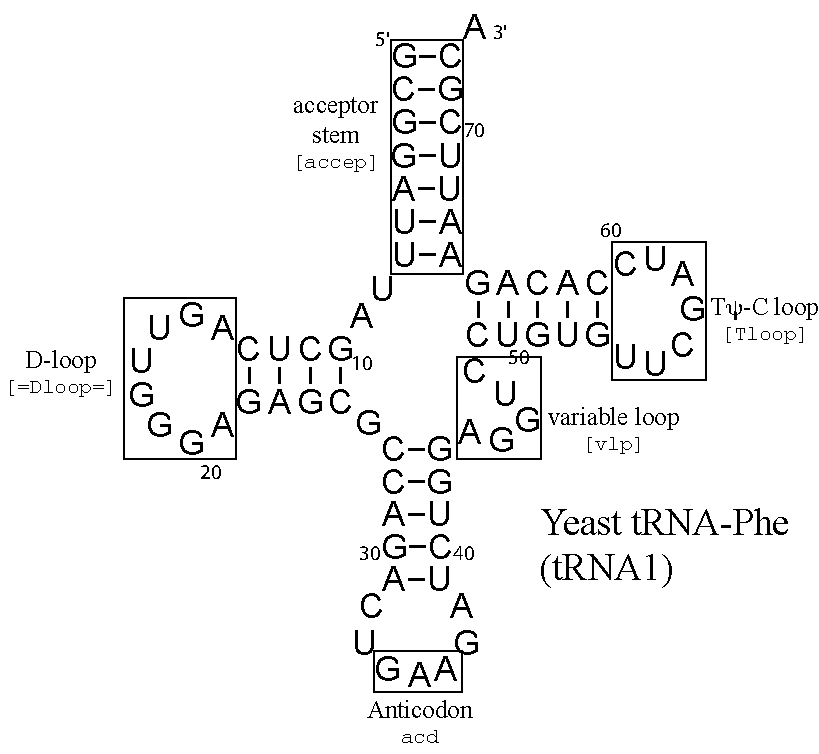
\includegraphics[scale=0.4]{Figures/trna1-DF6280-hand}
\end{minipage}
\vspace{1em}

This file is the same as \otext{tutorial/tRNA5.sto} except for the two
additional lines beginning with \otext{\#=GC RF}. This RF (reference)
annotation is required for using \otext{--hand}. When \otext{--hand}
is used, any non-gap character in the reference annotation will be
assigned as a match (consensus) position. Importantly, four different
characters are considered gaps: dashes (\otext{-}), underscores
(\otext{\_}), dots (\otext{.}) and tildes (\verb+~+). In this example
alignment, all columns are non-gap characters, so all columns will be
considered match positions.

Different regions of the secondary structure have been marked up using
abbreviations for the names of the regions in the reference
annotation. For example, \otext{acd} annotates the three positions of
the anticodon, and \otext{[vlp]} annotates the so-called variable
loop. I've used \otext{[} and \otext{]} to indicate region boundaries
in some cases. Crucially, I've avoided the use of any gap characters
for positions between named regions which I still want to be
considered match positions, and opted to use \otext{=} (which is not
considered a gap by \prog{cmbuild}) for these positions.

To build the hand-specified model from this alignment, do:

\user{cmbuild --hand tRNA5-hand.cm tutorial/tRNA5-hand.sto}

\begin{sreoutput}
# cmbuild :: covariance model construction from multiple sequence alignments
# INFERNAL 1.1.4 (Dec 2020)
# Copyright (C) 2020 Howard Hughes Medical Institute.
# Freely distributed under the BSD open source license.
# - - - - - - - - - - - - - - - - - - - - - - - - - - - - - - - - - - - -
# CM file:                                            tRNA5-hand.cm
# alignment file:                                     tutorial/tRNA5-hand.sto
# use #=GC RF annotation to define consensus columns: yes
# - - - - - - - - - - - - - - - - - - - - - - - - - - - - - - - - - - - -
#                                                                      rel entropy
#                                                                      -----------
# idx    name                     nseq eff_nseq   alen  clen  bps bifs    CM   HMM description
# ------ -------------------- -------- -------- ------ ----- ---- ---- ----- ----- -----------
       1 tRNA5-hand                  5     3.59     74    74   21    2 0.763 0.476 
#
# CPU time: 0.33u 0.01s 00:00:00.34 Elapsed: 00:00:00.35
\end{sreoutput}

The output reports that the model now has 74 match (consensus)
positions in the \otext{clen} column. If we had built this model
without specifying \otext{--hand} (as we did earlier in this tutorial)
the resulting model would have had only 72 consensus positions.
(I've annotated the two extra match positions with three gaps in
\otext{tRNA5.hand.sto} as match solely to demonstrate how
\otext{--hand} works, not because I think it's better to model these
positions as matches than inserts.)

Now, let's use this model to search the \emph{M. ruminantium} genome
again. First, the model must be calibrated. To save time, a calibrated
version of the file is in \otext{tutorial/tRNA5-hand.c.cm}. To do the
search:

\user{cmsearch tutorial/tRNA5-hand.c.cm tutorial/mrum-genome.fa}

The results are very similar to the earlier search with the
tRNA model built with default \prog{cmbuild} parameters (though not
identical since the model now has two additional match positions). The
important difference involves the hit alignments. Take a look at the
alignment for hit number 46 as an illustrative example:

\newpage

\begin{widesreoutput}
>> NC_013790.1  Methanobrevibacter ruminantium M1 chromosome, complete genome
 rank     E-value  score  bias mdl mdl from   mdl to       seq from      seq to       acc trunc   gc
 ----   --------- ------ ----- --- -------- --------    ----------- -----------      ---- ----- ----
 (46) !   1.6e-09   43.2   0.0  cm        1       74 []      995344      995263 - .. 0.90    no 0.49

                                 v          v                                                            NC
                     (((((((,,<<<<________._>>>>,<<<<<_______>>>>>,,,........,,<<<<<_______>>>>>))))))): CS
   tRNA5-hand      1 gCcggcaUAGcgcAgUUGGuu.AgcgCgccagccUgucAagcuggAGg........UCCgggGUUCGAUUCcccGugccgGca 74    
                     :::G:CAUAGCG AG  GGU+ A CGCG:CAG:CU +++A:CUG: G+        UC:GGGGUUCGA UCCCC:UG:C:::A
  NC_013790.1 995344 AGAGACAUAGCGAAGC-GGUCaAACGCGGCAGACUCAAGAUCUGUUGAuuaguucuUCAGGGGUUCGAAUCCCCUUGUCUCUA 995263
                     ************9***.8886258***********************9444444445************************** PP
                     [accep]======[=Dloop=.]============acd=======[vl........p]=====[Tloop]=====[accep]= RF
\end{widesreoutput}

The reference annotation from the training alignment to \prog{cmbuild}
has been propagated to the hit as an extra \otext{RF} line at the
bottom of the alignment. All inserts in the alignment are annotated as
\otext{.} columns in the RF annotation. Note that the variable loop
(annotated as \otext{[vlp]} in the training alignment) contains 8
inserted residues. The RF annotation will also be transferred to
multiple alignments created with \prog{cmalign}.


\section{The HMMER profile/sequence comparison pipeline}
\label{section:pipeline}
\setcounter{footnote}{0}

In this section, we briefly outline the processing pipeline for a
single profile/sequence comparison.\footnote{Code gurus and
  masochists: you can follow along in \ccode{src/p7\_pipeline.c}.} This
should help give you a sense of what HMMER is doing under the hood,
what sort of mistakes it may make (rarely, of course!), and what the
various results in the output actually mean. We'll first describe the 
pipeline in the context of protein search (\prog{phmmer}, \prog{hmmsearch},
\prog{hmmscan}, \prog{jackhmmer}), then wrap back around to discuss the
modified pipeline used in \prog{nhmmer} and \prog{nhmmscan}.


In briefest outline, the comparison pipeline takes the following
steps:

\begin{description}
\item[\textbf{Null model.}] Calculate a score term for the ``null
  hypothesis'' (a probability model of \emph{non-}homology). This
  score correction is used to turn all subsequent profile/sequence bit
  scores into a final log-odds bit score.
  
\item[\textbf{MSV filter.}] The main acceleration heuristic. The MSV
  (``Multiple Segment Viterbi'') algorithm looks for one or more
  high-scoring \emph{ungapped} alignments. If the MSV score passes a
  set threshold, the entire sequence passes on to the next pipeline
  step; else it is rejected.

\item[\textbf{Bias filter.}] A hack that reduces false positive MSV
  hits due to biased composition sequences. A two-state HMM is
  constructed from the mean residue composition of the profile and the
  standard residue composition of the null model, and used to score
  the sequence. The MSV bit score is corrected using this as a second
  null hypothesis. If the MSV score still passes the MSV threshold,
  the sequence passes on to the next step; else it is rejected.  The
  bias filter score correction will also be applied to the Viterbi
  filter and Forward filter scores that follow.
  
\item[\textbf{Viterbi filter.}] A more stringent accelerated filter.
  An optimal (maximum likelihood) gapped alignment score is
  calculated. If this score passes a set threshold, the sequence
  passes to the next step; else it is rejected.

\item[\textbf{Forward filter/parser.}] The full likelihood of the
  profile/sequence comparison is evaluated, summed over the entire
  alignment ensemble, using the HMM Forward algorithm. This score is
  corrected to a bit score using the null model and bias filter
  scores. If the bit score passes a set threshold, the sequence passes
  on to the next step; else it is rejected.

\item[\textbf{Domain identification.}] Using the Forward parser
  results, now combined with a Backward parser, posterior
  probabilities of domain locations are calculated. A discrete set of
  putative domains (alignments) is identified by applying heuristics
  to posterior probabilities. This procedure identifies
  \emph{envelopes}: subsequences on the target sequence which contain
  a lot of probability mass for a match to the profile.

\item[\textbf{Alignment.}] For each identified domain, a full
  Forward/Backward algorithm is performed. An \emph{ad hoc} ``null2''
  hypothesis is constructed for each domain's composition and used to
  calculate a biased composition score correction. A maximum expected
  accuracy (MEA) alignment is calculated. This identifies one MEA
  alignment within each envelope.

\item[\textbf{Storage.}] Now we have a \emph{sequence score} (and
  P-value); the sequence contains one or more domains, each of which
  has a \emph{domain score} (and P-value), and each domain has an MEA
  alignment annotated with per-residue posterior probabilities.

\end{description}

In more detail, each step is described in subsections that follow. Even more
detail may be found in \citep{Eddy11}.

\subsection{Null model.}

The ``null model'' calculates the probability that the target sequence
is \emph{not} homologous to the query profile. A HMMER bit score is
the log of the ratio of the sequence's probability according to the
profile (the homology hypothesis) over the null model probability (the
non-homology hypothesis). 

The null model is a one-state HMM configured to generate ``random''
sequences of the same mean length $L$ as the target sequence, with
each residue drawn from a background frequency distribution (a
standard i.i.d. model: residues are treated as independent and
identically distributed). Currently, this background frequency
distribution is hardcoded as the mean residue frequencies in Swiss-Prot
50.8 (October 2006).

For technical reasons, HMMER incorporates the \emph{residue emission}
probabilities of the null model directly into the profile, by turning
each emission probability in the profile into an odds ratio. The null
model score calculation therefore is only concerned with accounting
for the remaining \emph{transition} probabilities of the null model
and toting them up into a bit score correction.  The null model
calculation is fast, because it only depends on the length of the
target sequence, not its sequence.

\subsection{MSV filter.}

The sequence is aligned to the profile using a specialized model that
allows multiple high-scoring local ungapped segments to match.  The
optimal alignment score (Viterbi score) is calculated under this
multisegment model, hence the term MSV, for ``multi-segment
Viterbi''. This is HMMER's main speed heuristic.

The MSV score is comparable to BLAST's sum score (optimal sum of
ungapped alignment segments).  Roughly speaking, MSV is comparable to
skipping the heuristic word hit and hit extension steps of the BLAST
acceleration algorithm. 

The MSV filter is very, very fast. In addition to avoiding indel 
calculations in the dynamic programming table, it uses reduced precision
scores scaled to 8-bit integers, enabling acceleration via 16-way       
parallel SIMD vector instructions. 

The MSV score is a true log-odds likelihood ratio, so it obeys
conjectures about the expected score distribution \citep{Eddy08} that
allow immediate and accurate calculation of the statistical
significance (P-value) of the MSV bit score.

By default, comparisons with a P-value of $\leq$ 0.02 pass this
filter, meaning that about $2\%$ of nonhomologous sequences are
expected to pass. You can use the \ccode{--F1 <x>} option to change
this threshold. For example, \ccode{--F1 <0.05>} would pass 5\% of the
comparisons, making a search more sensitive but slower. Setting the
threshold to $\ge 1.0$ (\ccode{--F1 99} for example) assures that all
comparisons will pass. Shutting off the MSV filter may be worthwhile
if you want to make sure you don't miss comparisons that have a lot of
scattered insertions and deletions. Alternatively, the \ccode{--max}
option causes the MSV filter step (and all other filter steps) to be
bypassed.

The MSV bit score is calculated as a log-odds score using the null
model for comparison. No correction for a biased composition or
repetitive sequence is done at this stage. For comparisons involving
biased sequences and/or profiles, more than 2\% of comparisons will
pass the MSV filter. At the end of search output, there is a line
like:

\begin{sreoutput}
 Passed MSV filter:                    107917  (0.020272); expected 106468.8 (0.02)
\end{sreoutput}

 which tells you how many and what fraction of comparisons passed the
 MSV filter, versus how many (and what fraction) were expected. 


\subsection{Biased composition filter.}

It's possible for profiles and/or sequences to have biased residue
compositions that result in ``significant'' log-odds bit scores not
because the profile matches the sequence particularly well, but
because the \emph{null model} matches the sequence particularly badly.

HMMER uses fairly good methods to compensate its scores for biased
composition, but these methods are computationally expensive and
applied late in the pipeline (described below).

In a few cases, profiles and/or target sequences are sufficiently
biased that too many comparisons pass the MSV filter, causing HMMER
speed performance to be severely degraded. Although the final scores
and E-values at the end of the pipeline will be calculated taking into
account a ``null2'' model of biased composition and simple repetition,
the null2 model is dependent on a full alignment ensemble calculation
via the Forward/Backward algorithm, making it computationally complex,
so it won't get calculated until the very end. The treatment of biased
composition comparisons is probably the most serious problem remaining
in HMMER. Solving it well will require more research. As a stopgap
solution to rescuing most of the speed degradation while not
sacrificing too much sensitivity, an \emph{ad hoc} biased composition
filtering step is applied to remove highly biased comparisons.

On the fly, a two-state HMM is constructed. One state emits residues
from the background frequency distribution (same as the null1 model),
and the other state emits residues from the mean residue composition
of the profile (i.e. the expected composition of sequences generated
by the core model, including match and insert states
[\ccode{p7\_hmm.c:p7\_hmm\_SetComposition()}]). Thus if the profile is
highly biased (cysteine-rich, for example; or highly hydrophobic with
many transmembrane segments), this composition bias will be captured
by this second state. This model's transitions are arbitrarily set
such that state 1 emits an expected length of 400 at a time, and state
2 emits an expected length of M/8 at a time (for a profile of length
M). An overall target sequence length distribution is set to a mean of
$L$, identical to the null1 model.

The sequence is then rescored using this ``bias filter model'' in
place of the null1 model, using the HMM Forward algorithm. (This
replaces the null1 model score at all subsequent filter steps in the
pipeline, until a final Forward score is calculated.) A new MSV bit
score is obtained.

If the P-value of this still satisfies the MSV thresholds, the
sequence passes the biased composition filter. 

The \ccode{--F1 <x>} option controls the P-value threshold for
passing the MSV filter score, both before (with the simple null1
model) and after the bias composition filter is applied.

The \ccode{--max} option bypasses all filters in the pipeline,
including the bias filter.

The \ccode{--nobias} option turns off (bypasses) the biased
composition filter.  The simple null model is used as a null
hypothesis for MSV and in subsequent filter steps. The biased
composition filter step compromises a small amount of sensitivity.
Though it is good to have it on by default, you may want to shut it
off if you know you will have no problem with biased composition hits.

 At the end of a search output, you will see a line like:

\begin{sreoutput}
 Passed bias filter:                   105665  (0.019849); expected 106468.8 (0.02)
\end{sreoutput}

which tells you how many and what fraction of comparisons passed the
biased composition filter, versus how many were expected. (If the
filter was turned off, all comparisons pass.)


\subsection{Viterbi filter.}

The sequence is now aligned to the profile using a fast Viterbi
algorithm for optimal gapped alignment.

This Viterbi implementation is specialized for speed.  It is
implemented in 8-way parallel SIMD vector instructions, using reduced
precision scores that have been scaled to 16-bit integers. Only one
row of the dynamic programming matrix is stored, so the routine only
recovers the score, not the optimal alignment itself. The reduced
representation has limited range; local alignment scores will not
underflow, but high scoring comparisons can overflow and return
infinity, in which case they automatically pass the filter.

The final Viterbi filter bit score is then computed using the
appropriate null model log likelihood (by default the biased
composition filter model score, or if the biased filter is off, just
the null model score). If the P-value of this score passes the Viterbi
filter threshold, the sequence passes on to the next step of the
pipeline.
 
The \ccode{--F2 <x>} option controls the P-value threshold for passing
the Viterbi filter score. The default is 0.001.
The \ccode{--max} option bypasses all filters in the pipeline.


At the end of a search output, you will see a line like:

\begin{sreoutput}
Passed Vit filter:                      2207  (0.00443803); expected 497.3 (0.001)
\end{sreoutput}

which tells you how many and what fraction of comparisons passed the
Viterbi filter, versus how many were expected.
 
  

\subsection{Forward filter/parser.}

The sequence is now aligned to the profile using the full Forward
algorithm, which calculates the likelihood of the target sequence
given the profile, summed over the ensemble of all possible
alignments.

This is a specialized time- and memory-efficient Forward
implementation called the ``Forward parser''. It is implemented in
4-way parallel SIMD vector instructions, in full precision (32-bit
floating point). It stores just enough information that, in
combination with the results of the Backward parser (below), posterior
probabilities of start and stop points of alignments (domains) can be
calculated in the domain definition step (below), although the
detailed alignments themselves cannot be.

The Forward filter bit score is calculated by correcting this score
using the appropriate null model log likelihood (by default the biased
composition filter model score, or if the biased filter is off, just
the null model score). If the P-value of this bit score passes the
Forward filter threshold, the sequence passes on to the next step of
the pipeline.

The bias filter score has no further effect in the pipeline. It is
only used in filter stages. It has \emph{no} effect on final reported
bit scores or P-values. Biased composition compensation for final bit
scores is done by a more complex domain-specific algorithm, described
below.

The \ccode{--F3 <x>} option controls the P-value threshold for passing
the Forward filter score. The default is 1e-5.  The \ccode{--max}
option bypasses all filters in the pipeline.

At the end of a search output, you will see a line like:

\begin{sreoutput}
Passed Fwd filter:                      1076  (0.00216371); expected 5.0 (1e-05)
\end{sreoutput}

which tells you how many and what fraction of comparisons passed the
Forward filter, versus how many were expected.


\subsection{Domain definition.}

A target sequence that reaches this point is very likely to contain
one or more significant matches to the profile. These matches are
referred to as ``domains'', since the main use of HMMER has
historically been to match profile HMMs from protein domain databases
like Pfam, and one of HMMER's strengths is to be able to cleanly parse
a multidomain target sequence into its multiple nonoverlapping hits to
the same domain model.

The domain definition step is essentially its own pipeline, with steps
as follows:\footnote{Code gurus and masochists can follow along in 
\ccode{src/p7\_domaindef.c}.}

\paragraph{Backward parser.}
The counterpart of the Forward parser algorithm is calculated in an
analogous time- and memory-efficient implementation. The Forward
algorithm gives the likelihood of all \emph{prefixes} of the target
sequence, summed over their alignment ensemble, and the Backward
algorithm gives the likelihood of all \emph{suffixes}. For any given
point of a possible model state/residue alignment, the product of the
Forward and Backward likelihoods gives the likelihood of the entire
alignment ensemble conditional on using that particular alignment
point. Thus, we can calculate things like the posterior probability
that an alignment starts or ends at a given position in the target
sequence.

\paragraph{Domain decoding.}
The posterior decoding algorithm is applied, to calculate the
posterior probability of alignment starts and ends (profile B and E
state alignments) with respect to target sequence position.

The sum of the posterior probabilities of alignment starts (B states)
over the entire target sequence is the \emph{expected number of
  domains} in the sequence.

In a tabular output (\ccode{--tblout}) file, this number is in the
column labeled \ccode{exp}.

\paragraph{Region identification.}

A heuristic is now applied to identify a \emph{non-overlapping} set of
``regions'' that contain significant probability mass suggesting the
presence of a match (alignment) to the profile.

For each region, the expected number of domains is calculated (again
by posterior decoding on the Forward/Backward parser results). This
number should be about 1: we expect each region to contain one local
alignment to the profile. 

In a tabular output (\ccode{--tblout}) file, the number of discrete
regions identified by this posterior decoding step is in the column
labeled \ccode{reg}. It ought to be almost the same as the expectation
\ccode{exp}. If it is not, there may be something funny going on, like
a tandem repetitive element in the target sequence (which can produce
so many overlapping weak hits that the sequence appears to be a
significant hit with lots of domains expected \emph{somewhere}, but
the probability is fuzzed out over the repetitive region and few or no
good discrete alignment regions can be identified).

\paragraph{Envelope identification.}

Now, within each region, we will attempt to identify \emph{envelopes}.
An \emph{envelope} is a subsequence of the target sequence that
appears to contain alignment probability mass for a likely domain (one
local alignment to the profile).

When the region contains $\simeq$1 expected domain, envelope
identification is already done: the region's start and end points are
converted directly to the envelope coordinates of a putative domain.

There are a few cases where the region appears to contain more than
one expected domain -- where more than one domain is closely spaced on
the target sequence and/or the domain scores are weak and the
probability masses are ill-resolved from each other. These
``multidomain regions'', when they occur, are passed off to an even
more \emph{ad hoc} resolution algorithm called \emph{stochastic
  traceback clustering}. In stochastic traceback clustering, we sample
many alignments from the posterior alignment ensemble, cluster those
alignments according to their overlap in start/end coordinates, and
pick clusters that sum up to sufficiently high probability. Consensus
start and end points are chosen for each cluster of sampled
alignments. These start/end points define envelopes.

These envelopes identified by stochastic traceback clustering are
\emph{not} guaranteed to be nonoverlapping. It's possible that there
are alternative ``solutions'' for parsing the sequence into domains,
when the correct parsing is ambiguous. HMMER will report all
high-likelihood solutions, not just a single nonoverlapping parse.

It's also possible (though rare) for stochastic clustering to identify
\emph{no} envelopes in the region.

In a tabular output (\ccode{--tblout}) file, the number of regions
that had to be subjected to stochastic traceback clustering is given
in the column labeled \ccode{clu}. This ought to be a small number
(often it's zero). The number of envelopes identified by stochastic
traceback clustering that overlap with other envelopes is in the
column labeled \ccode{ov}. If this number is non-zero, you need to be
careful when you interpret the details of alignments in the output,
because HMMER is going to be showing overlapping alternative
solutions. The total number of domain envelopes identified (either by
the simple method or by stochastic traceback clustering) is in the
column labeled \ccode{env}. It ought to be almost the same as the
expectation and the number of regions.

\paragraph{Maximum expected accuracy alignment.}
Each envelope is now aligned to the profile using the full
Forward/Backward algorithm. The profile is configured to ``unihit''
mode, so that the profile expects only one local alignment (domain) in
the envelope (as opposed to multiple domains).  Posterior decoding is
used to calculate the posterior probability of every detailed
alignment of profile state to sequence residue. The posterior
decodings are used to extract a ``maximum expected accuracy''
alignment. Each aligned residue is annotated with its posterior
probability in the Forward/Backward alignment ensemble.

Currently, the Forward, Backward, and posterior decoding calculations
at this step are \emph{not} memory efficient. They calculate matrices
requiring roughly $36 ML$ bytes, where $M$ is the profile length and
$L$ is the length of the envelope subsequence. Usually in
\prog{hmmsearch} and \prog{hmmscan}, profiles and envelopes are small
enough that this is not a problem. For example, a typical Pfam domain
model is about 200 residues long, matching to individual target
envelopes of about 200 residues each; this requires about 1.4 MB of
memory in MEA alignment. However, in \prog{phmmer} and
\prog{jackhmmer} programs, it's often going to be the case that you're
aligning an entire query sequence to an entire target sequence in a
single unresolved ``domain'' alignment. If this is titin (about 40,000
residues), it would require 57.6 GB of RAM. For this reason,
currently, \prog{phmmer} and \prog{jackhmmer} can only handle query
sequences of up to a few thousand residues. If you see a ``fatal
exception'' error complaining about failure of a large memory
allocation, you're almost certainly seeing a prohibitive memory
requirement at this stage.\footnote{We know how to fix this, with
  memory-efficient algorithms, and are working on it.}

In a tabular output (\ccode{--tblout}) file, the number of domains in
envelopes (before any significance thresholding) is in the column
labeled \ccode{dom}. This will generally be the same as the number of
envelopes.

\paragraph{Biased composition score correction (``null2'')}
An \emph{ad hoc} biased composition score correction is calculated for
each envelope, using the posterior decoding. A corrected bit score and
P-value for each envelope is calculated. These null2-corrected scores
are subjected to the reporting and inclusion thresholds, at both the full
sequence level and per-domain.

%Once the position-specific ``null2'' score is available, specifying a
%biased composition correction that applies to every residue, the total
%corrected bit score for the target sequence is recalculated, by
%summing up envelope scores for each significant domain.



\subsection{Modifications to the pipeline as used for DNA search.}

\subsubsection{SSV, not MSV.}

In the MSV filter, one or more high-scoring ungapped segments contribute to a
score that, if sufficiently high, casues the entire sequence to be passed on to
the next stage (the bias filter). This strategy won't work for long
DNA sequences; it doesn't filter the human genome much to say ``there's a hit on
chromosome 1, now process the whole thing''. In the scanning-SSV (``Single
ungapped Segment Viterbi'') algorithm used in \prog{nhmmer} and
\prog{nhmmscan}, each comparison between a query and target is
scanned for high-scoring ungapped alignment segments, and a window around each 
such segment is extracted, merging overlapping windows. Each window is then
passed on to the remaining filter cascade, where it is (for the most part)
treated as described above. As with the MSV filter, the default P-value 
threshold is $0.02$, and can be controlled with the \ccode{--F1} flag.

The \ccode{--max} flag also controls the amount of the sequence database that
passes the SSV filter, but instead of the threshold being set to $1.0$, as
described for the protein pipeline, it is set to $0.4$.
%, which allows passage to anything with a sniff of a chance of passing the
% final threshold

%Without doing this, the
%segment-surrounding windows all overlap to the point that merging them causes
%full-length chromosomes to possibly trickle down to the later
%envelope-definition machinery, causing to out-of-memory errors. As a special
%hack in case of very long merged windows, a maximum window length of 80Kb is
%enforced by splitting long windows (keeping overlapping blocks, and tracking
%shared hits as necessary to avoid duplicates).


\subsubsection{There are no domains, but there are envelopes.}

In HMMER's protein-search programs, multiple matches of the model to a target
sequence are treated as domains contained within a single hit for that
sequence. In the DNA-search programs, each match of the model to a subsequence
is treated as an independent hit - there's no notion of a domain. This is
largely a difference in reporting; both pipelines rely on essentially the same 
envelope detection code; envelopes lead to domains in protein search, and
hits in DNA search.


\subsubsection{Biased composition.}

DNA sequence is littered with regions containing tandem simple repeats or other 
low complexity sequence. Without accounting for such composition bias, we see
many cases in which one part of a hit is obviously legitimate, and serves as the
anchor for a neighboring alignment segment that is clearly low-complexity
garbage, one form of a problem known as homologous overextension
\citep{Gonzalez10}. The null2 method used in protein search delays score
modification until after the alignment is complete, but we know that
this kind of overextension can be (mostly) avoided if the model's log odds
scores account for the composition bias of the target region while constructing
the alignment. The DNA search pipeline therefore does just this: it modifies
the scoring scheme for each target envelope as a function of that envelope's
sequence composition, then builds the alignment according to that scheme.


%\subsubsection{More about envelopes.}

%DNA sequence is littered with regions containing tandem simple repeats or other 
%low complexity sequence. When an HMM contains a regions with similar bias, the
%envelope-definition machinery can produce absurdly long envelopes
%around plausible alignments\footnote{we've seen envelopes extending more than
%1000 bases beyond the end of an alignment of length 300}. This happens because
%the region-identification method is confused: there are many overlapping weak
%hits, with no discrete alignment good enough to call a hit. 

%By trimming these very long envelopes such that they are no more than 20 bases
%beyond the edges of the aligned range, \ldots 


\section{Tabular output formats}
\label{section:tabular}
\setcounter{footnote}{0}

\subsection{Target hits tables}

The \ccode{--tblout} output option in \prog{cmsearch} and
\prog{cmscan} produces \emph{target hits tables}. There are two
different formats of target hits table, which are both described
below. By default, both \prog{cmsearch} and \prog{cmscan} produce the
target hits table in \emph{format 1}. Format 1 is the only format that
was used by Infernal versions 1.1rc1 through 1.1.1. As of version 1.1.2,
with \prog{cmscan}, the \ccode{--fmt 2} option can be used in
combination with \ccode{--tblout} to produce a target hits table in
the alternative \emph{format 2}.  Both formats 1 and 2 target hits
table consist of one line for each different query/target comparison
that met the reporting thresholds, ranked by decreasing statistical
significance (increasing E-value).

\subsubsection{Target hits table format 1}

In the format 1 table, each line
consists of \textbf{18 space-delimited fields} followed by a free text
target sequence description, as follows:\footnote{The \ccode{tblout}
  format is deliberately space-delimited (rather than tab-delimited)
  and justified into aligned columns, so these files are suitable both
  for automated parsing and for human examination. Tab-delimited data
  files are difficult for humans to examine and spot check. For this
  reason, we think tab-delimited files are a minor evil in the
  world. Although we occasionally receive shrieks of outrage about
  this, we stubbornly feel that space-delimited files are just as
  trivial to parse as tab-delimited files.}

\begin{description}
\item[\emprog{(1) target name:}]
  The name of the target sequence or profile. 

\item[\emprog{(2) accession:}]
  The accession of the target sequence or profile, or '-' if none.

\item[\emprog{(3) query name:}] 
  The name of the query sequence or profile.

\item[\emprog{(4) accession:}]
  The accession of the query sequence or profile, or '-' if none.

\item[\emprog{(5) mdl (model):}] Which type of model was used to
  compute the final score. Either 'cm' or 'hmm'. A CM is
  used to compute the final hit scores unless the model has zero
  basepairs or the \ccode{--hmmonly} option is used, in which case a
  HMM will be used. 

\item[\emprog{(6) mdl from (model coord):}]
  The start of the alignment of this hit with respect to the
  profile (CM or HMM), numbered 1..N for a profile of N consensus positions.

\item[\emprog{(7) mdl to (model coord):}]
  The end of the alignment of this hit with respect to the
  profile (CM or HMM), numbered 1..N for a profile of N consensus positions.

\item[\emprog{(8) seq from (ali coord):}]
  The start of the alignment of this hit with respect to the
  sequence, numbered 1..L for a sequence of L residues.
 
\item[\emprog{(9) seq to (ali coord):}]
  The end of the alignment of this hit with respect to the
  sequence, numbered 1..L for a sequence of L residues.

\item[\emprog{(10) strand:}]
  The strand on which the hit occurs on the sequence. '+' if the hit is on
  the top (Watson) strand, '-' if the hit is on the bottom (Crick) strand.
  If on the top strand, the ``seq from'' value will be less than or
  equal to the ``seq to'' value, else it will be greater than or equal
  to it. 

\item[\emprog{(11) trunc:}] 
  Indicates if this is predicted to be a truncated CM hit or not. This will be
  ``no'' if it is a CM hit that is not predicted to be truncated by the end of the
  sequence, ``5'\,'' or ``3'\,'' if the hit is predicted to have one or more
  5' or 3' residues missing  due to a artificial truncation of the
  sequence, or ``5'\&3''' if the hit is predicted to have one or more
  5' residues missing and one or more 3' residues missing.
  If the hit is an HMM hit, this will always be '-'. 

\item[\emprog{(12) pass:}] 
  Indicates what ``pass'' of the pipeline the hit was detected
  on. This is probably only useful for testing and
  debugging. Non-truncated hits are found on the first pass, truncated
  hits are found on successive passes.

\item[\emprog{(13) gc:}] 
  Fraction of G and C nucleotides in the hit. 

\item[\emprog{(14) bias:}] The biased-composition correction: the bit
  score difference contributed by the null3 model for CM hits, or the
  null2 model for HMM hits. High bias scores may be a red flag for a
  false positive. It is difficult to correct for all possible ways in
  which a nonrandom but nonhomologous biological sequences can appear
  to be similar, such as short-period tandem repeats, so there are
  cases where the bias correction is not strong enough (creating false
  positives).

\item[\emprog{(15) score:}]
  The score (in bits) for this target/query comparison. It includes
  the biased-composition correction (the ``null3'' model for CM hits,
  or the ``null2'' model for HMM hits). 

\item[\emprog{(16) E-value:}] The expectation value (statistical
  significance) of the target.  This is a \emph{per query} E-value;
  i.e.\ calculated as the expected number of false positives achieving
  this comparison's score for a \emph{single} query against the search
  space $Z$. For \prog{cmsearch} $Z$ is defined as the total number of
  nucleotides in the target dataset multiplied by 2 because both strands
  are searched. For \prog{cmscan} $Z$ is the total number of
  nucleotides in the query sequence multiplied by 2 because both
  strands are searched and multiplied by the number of models in the target
  database. If you search with multiple queries and if you want to
  control the \emph{overall} false positive rate of that search rather
  than the false positive rate per query, you will want to multiply
  this per-query E-value by how many queries you're doing.

\item[\emprog{(17) inc:}] 
  Indicates whether or not this hit achieves the inclusion threshold:
  '!' if it does, '?' if it does not (and rather only achieves the
  reporting threshold). By default, the inclusion threshold is an
  E-value of 0.01 and the reporting threshold is an E-value of 10.0,
  but these can be changed with command line options as described in
  the manual pages.

\item[\emprog{(18) description of target:}] 
  The remainder of the line is the target's description line, as free text.
\end{description}

\subsubsection{Target hits table format 2}
\label{tabular-format2}

Format 2 includes all 18 of the fields from format 1 in the same order, plus 9
additional fields that are interspersed between some of the 18 from
format 1, as follows:

\begin{description}

\item[\emprog{(Before field 1 of format 1) idx:}] 
  The index of the hit in the list. The first hit has index '1', the
  second has index '2', the Nth hit has index 'N'.

\item[\emprog{(Before field 5 of format 1) clan name:}] 
  The name of the clan the model for this hit belongs to, or \ccode{-} if
  the model does not belong to a clan. A clan is a group of related
  models. For example, Rfam groups three LSU rRNA models
  (LSU\_rRNA\_archaea, LSU\_rRNA\_bacteria, and LSU\_rRNA\_eukarya)
  into the same clan. The value in this field will always be \ccode{-}
  unless the \ccode{--clanin <f>} option was used with
  \ccode{cmscan} to specify clan/model relationships in the input file
  \ccode{<f>}. See section~\ref{section:formats} for a description of
  the format of the input file used with \ccode{--clanin}.

\end{description}

The following seven fields all occur in format 2 between fields 17
('inc:') and 18 ('description of target') from format 1. 

\begin{description}

\item[\emprog{olp:}] A single character indicating the overlap status
  of this hit. Here, two hits are deemed to \emph{overlap} if they
  share at least one nucleotide on the same strand of the same
  sequence. There are three possible values in this field: \ccode{*},
  \ccode{\^} and \ccode{=}.  \ccode{*} indicates this hit does not
  overlap with any other reported hits. \ccode{\^} indicates that this
  hit does overlap with at least one other hit, but none of the hits
  that overlap with it have a higher score (occur above it in the hit
  list). \ccode{=} indicates that this hit does overlap with at least
  one other hit that has a higher score (occurs above it in the hit
  list). If the \ccode{--oclan} option was enabled, the definition of
  \emph{overlap} for the designations of the three characters
  \ccode{*}, \ccode{\^} and \ccode{=} described above changes to: two
  hits are deemed to \emph{overlap} if they share at least one
  nucleotide on the same strand of the same sequence and they are to
  models that are in the same clan. That is, only overlaps between
  hits to models that are in the same clan are counted, all other
  overlaps are ignored and not annotated.  Infernal will never report
  two overlapping hits to the same model.

\item[\emprog{anyidx:}]
For hits that have \ccode{=} in the ``olp'' field, this is the
index of the best scoring hit that overlaps with this hit.
For hits with either \ccode{*} or \ccode{\^} in the "olp" field,
this field will always be \ccode{-}.

\item[\emprog{anyfrct1:}]
For hits that have \ccode{=} in the "olp" field, this is the
fraction of the length of this hit that overlaps with the best scoring
overlapping hit (the hit index given in the "anyidx" field), to
4 significant digits. 
For hits with \ccode{-} in the "anyidx"
field, this field will always be \ccode{-}.  

\item[\emprog{anyfrct2:}]
For hits that have \ccode{=} in the "olp" field, this is the
fraction of the length of the best scoring overlapping hit (the hit
index given in the "anyidx" field) that overlaps with this hit,
to 4 significant digits. 
For hits with \ccode{-} in the "anyidx"
field, this field will always be \ccode{-}.  

\item[\emprog{winidx:}] 
For hits that have \ccode{=} in the "olp" field, this is either
\ccode{"} or the index of the best scoring hit that overlaps with this
hit that is marked as \ccode{\^} in the "olp" field. If the value
is \ccode{"} it means that the best scoring hit that overlaps with
this hit that is marked as \ccode{\^} in the "olp" field is
already listed in the "anyidx" field, which is usually the case.
For hits with either \ccode{*} or \ccode{\^} in the "olp" field,
this field will always be \ccode{-}.

\item[\emprog{winfrct1:}]
For hits that have neither \ccode{-} nor \ccode{"} in the
"winidx" field, this is the fraction of the length of this hit
that overlaps with the best scoring overlapping hit marked with
\ccode{\^} in the "olp" field (the hit index given in the
"winidx" field), to 4 significant digits.  For hits with either
\ccode{*} or \ccode{\^} in the "olp" field, this field will
always be \ccode{-}.  For hits with \ccode{-} in the "winidx"
field, this field will always be \ccode{-}.  
For hits with \ccode{"} in the "winidx"
field, this field will always be \ccode{"}.  

\item[\emprog{winfrct2:}]
For hits that have neither \ccode{-} nor \ccode{"} in the
"winidx" field, this is the
fraction of the length of the best scoring overlapping hit marked with
\ccode{\^} in the "olp" field (the hit
index given in the "winidx" field) that overlaps with this hit,
to 4 significant digits. 
  For hits with either
\ccode{*} or \ccode{\^} in the "olp" field, this field will
always be \ccode{-}.  For hits with \ccode{-} in the "winidx"
field, this field will always be \ccode{-}.  
For hits with \ccode{"} in the "winidx"
field, this field will always be \ccode{"}.  

\end{description}

The tables are columnated neatly for human readability, but do not
write parsers that rely on this columnation; rely on space-delimited
fields. The pretty columnation assumes fixed maximum widths for each
field. If a field exceeds its allotted width, it will still be fully
represented and space-delimited, but the columnation will be disrupted
on the rest of the row.

Note the use of target and query columns. A program like
\prog{cmsearch} searches a query profile against a target sequence
database. In an \prog{cmsearch} tblout file, the sequence (target)
name is first, and the profile (query) name is second. A program like
\prog{cmscan}, on the other hand, searches a query sequence against a
target profile database. In a \prog{cmscan} tblout file, the profile
name is first, and the sequence name is second. You might say, hey,
wouldn't it be more consistent to put the profile name first and the
sequence name second (or vice versa), so \prog{cmsearch} and
\prog{cmscan} tblout files were identical? Well, they
still wouldn't be identical, because the target database size used for
E-value calculations is different (total number of target nucleotides
for \prog{cmsearch}, number of target profiles times target sequence
length for \prog{cmscan}), and it's good not to forget this.

If some of the descriptions of these fields don't make sense to you,
it may help to go through the tutorial in
section~\ref{section:tutorial} and read section~\ref{section:pipeline}
of the manual. 



\begin{adjustwidth}{}{-1in}   
\chapter{Manual pages for HMMER programs}             
\input{manpages}
\end{adjustwidth}

\begin{adjustwidth}{}{-1in}   
\chapter{Manual pages for Easel miniapps}             
\input{easel_manpages}
\end{adjustwidth}

\section{File formats}
\label{section:formats}
\setcounter{footnote}{0}

\subsection{HMMER profile HMM files}
\label{section:savefiles}

The file \prog{tutorial/fn3.hmm} gives an example of a HMMER3 ASCII
save file. An abridged version is shown here, where (\ldots) mark
deletions made for clarity and space:

\begin{tinysreoutput}
HMMER3/f [3.1 | February 2013]
NAME  fn3
ACC   PF00041.13
DESC  Fibronectin type III domain
LENG  86
ALPH  amino
RF    no
MM    no
CONS  yes
CS    yes
MAP   yes
DATE  Fri Feb 15 06:04:13 2013
NSEQ  106
EFFN  11.415833
CKSUM 3564431818
GA    8.00 7.20
TC    8.00 7.20
NC    7.90 7.90
STATS LOCAL MSV       -9.4043  0.71847
STATS LOCAL VITERBI   -9.7737  0.71847
STATS LOCAL FORWARD   -3.8341  0.71847
HMM          A        C        D        E        F        G        H        I    (...)    Y   
            m->m     m->i     m->d     i->m     i->i     d->m     d->d
  COMPO   2.70330  4.91262  3.03272  2.64079  3.60307  2.84344  3.74204  3.07942 (...) 3.21526
          2.68618  4.42225  2.77519  2.73123  3.46354  2.40513  3.72494  3.29354 (...) 3.61503
          0.00338  6.08833  6.81068  0.61958  0.77255  0.00000        *
      1   3.16986  5.21447  4.52134  3.29953  4.34285  4.18764  4.30886  3.35801 (...) 3.93889      1 p - - -
          2.68629  4.42236  2.77530  2.73088  3.46365  2.40512  3.72505  3.29365 (...) 3.61514
          0.09796  2.38361  6.81068  0.10064  2.34607  0.48576  0.95510
      2   2.70230  5.97353  2.24744  2.62947  5.31433  2.60356  4.43584  4.79731 (...) 4.25623      3 s - - -
          2.68618  4.42225  2.77519  2.73123  3.46354  2.40513  3.72494  3.29354 (...) 3.61503
          0.00338  6.08833  6.81068  0.61958  0.77255  0.48576  0.95510
(...)
     85   2.48488  5.72055  3.87501  1.97538  3.04853  3.48010  4.51877  3.51898 (...) 3.43366    120 e - - B
     
          2.68618  4.42225  2.77519  2.73123  3.46354  2.40513  3.72494  3.29354 (...) 3.61503
          0.00338  6.08833  6.81068  0.61958  0.77255  0.48576  0.95510
     86   3.03720  5.94099  3.75455  2.96917  5.26587  2.91682  3.66571  4.11840 (...) 4.99111    121 s - - E
     
          2.68618  4.42225  2.77519  2.73123  3.46354  2.40513  3.72494  3.29354 (...) 3.61503
          0.00227  6.08723        *  0.61958  0.77255  0.00000        *
//
\end{tinysreoutput}

An HMM file consists of one or more HMMs.  Each HMM starts with a
format version identifier (here, \prog{HMMER3/f}) and ends with
\prog{//} on a line by itself.  The format version identifier allows
backward compatibility as the HMMER software evolves: it tells the
parser this file is from HMMER3's save file format version
f.\footnote{HMMER 3.0 used 3/b format. HMMER 3.1 uses 3/f format.
  Some alpha test versions of 3.0 used 3/a format. Internal
  development versions of 3.1 used 3/c, 3/d, and 3/e formats.}  The closing
\prog{//} allows multiple HMMs to be concatenated.

The format is divided into two regions. The first region contains
textual information and miscalleneous parameters in a roughly
tag-value scheme.  This section ends with a line beginning with the
keyword \prog{HMM}. The second region is a tabular, whitespace-limited
format for the main model parameters.

All probability parameters are all stored as negative natural log
probabilities with five digits of precision to the right of the
decimal point, rounded. For example, a probability of $0.25$ is stored
as $-\log 0.25 = 1.38629$. The special case of a zero probability is
stored as '*'.

Spacing is arranged for human readability, but the parser only cares
that fields are separated by at least one space character.

A more detailed description of the format follows.

\subsubsection{header section}

The header section is parsed line by line in a tag/value format. Each
line type is either \textbf{mandatory} or \textbf{optional} as
indicated. 

\begin{sreitems}{\emprog{header}}

\item [\emprog{HMMER3/f}] Unique identifier for the save file format
  version; the \prog{/f} means that this is HMMER3 HMM file format
  version f. When HMMER3 changes its save file format, the revision
  code advances. This way, parsers may easily remain backwards
  compatible. The remainder of the line after the \prog{HMMER3/f} tag
  is free text that is ignored by the parser. HMMER currently writes
  its version number and release date in brackets here,
  e.g. \prog{[3.1b2 | December 2013]} in this
  example. \textbf{Mandatory.}

\item [\emprog{NAME <s>}] Model name; \prog{<s>} is a single word
containing no spaces or tabs. The name is normally picked up from the
\verb+#=GF ID+ line from a Stockholm alignment file.  If this is not
present, the name is created from the name of the alignment file by
removing any file type suffix. For example, an otherwise nameless HMM
built from the alignment file \prog{rrm.slx} would be named
\prog{rrm}.  \textbf{Mandatory.}

\item [\emprog{ACC <s>}] Accession number; \prog{<s>} is a one-word
accession number. This is picked up from the \verb+#=GF AC+ line in a
Stockholm format alignment. \textbf{Optional.}

\item [\emprog{DESC <s>}] Description line; \prog{<s>} is a one-line
free text description. This is picked up from the \verb+#=GF DE+ line
in a Stockholm alignment file. \textbf{Optional.}

\item [\emprog{LENG <d>}] Model length; \prog{<d>}, a positive nonzero
integer, is the number of match states in the model.
\textbf{Mandatory.}

\item [\emprog{MAXL <d>}] Max instance length; \prog{<d>}, a positive
nonzero integer, is the upper bound on the length at which and instance
of the model is expected to be found. Used only by nhmmer and nhmmscan.
\textbf{Optional.}

\item [\emprog{ALPH <s>}] Symbol alphabet type. For biosequence
analysis models, \prog{<s>} is \prog{amino}, \prog{DNA}, or \prog{RNA}
(case insensitive). There are also other accepted alphabets for
purposes beyond biosequence analysis, including \prog{coins},
\prog{dice}, and \prog{custom}. This determines the symbol alphabet
and the size of the symbol emission probability distributions.  If
\prog{amino}, the alphabet size $K$ is set to 20 and the symbol
alphabet to ``ACDEFGHIKLMNPQRSTVWY'' (alphabetic order); if
\prog{DNA}, the alphabet size $K$ is set to 4 and the symbol alphabet
to ``ACGT''; if \prog{RNA}, the alphabet size $K$ is set to 4 and the
symbol alphabet to ``ACGU''. \textbf{Mandatory.}

\item [\emprog{RF <s>}] Reference annotation flag; \prog{<s>} is
either \prog{no} or \prog{yes} (case insensitive). If \prog{yes}, the
reference annotation character field for each match state in the main
model (see below) is valid; if \prog{no}, these characters are
ignored.  Reference column annotation is picked up from a Stockholm
alignment file's \verb+#=GC RF+ line. It is propagated to alignment
outputs, and also may optionally be used to define consensus match
columns in profile HMM construction. \textbf{Optional}; assumed to be
no if not present.

\item [\emprog{MM <s>}] Model masked flag; \prog{<s>} is
either \prog{no} or \prog{yes} (case insensitive). If \prog{yes}, the
model mask annotation character field for each match state in the main
model (see below) is valid; if \prog{no}, these characters are
ignored. Indicates that the profile model was created such that
emission probabilities at masked positions are set to match the 
background frequency, rather than being set based on observed frequencies 
in the alignment. Position-specific insertion and deletion rates are not 
altered, even in masked regions. \textbf{Optional}; assumed to be
no if not present.

\item [\emprog{CONS <s>}] Consensus residue annotation flag;
  \prog{<s>} is either \prog{no} or \prog{yes} (case insensitive).  If
  \prog{yes}, the consensus residue field for each match state in the
  main model (see below) is valid. If \prog{no}, these characters are
  ignored. Consensus residue annotation is determined when models are
  built. For models of single sequences, the consensus is the same as
  the query sequence. For models of multiple alignments, the consensus
  is the maximum likelihood residue at each position. Upper case
  indicates that the model's emission probability for the consensus
  residue is $\geq$ an arbitrary threshold (0.5 for protein models,
  0.9 for DNA/RNA models).

\item [\emprog{CS <s>}] Consensus structure annotation flag;
\prog{<s>} is either \prog{no} or \prog{yes} (case insensitive). If
\prog{yes}, the consensus structure character field for each match
state in the main model (see below) is valid; if \prog{no} these
characters are ignored. Consensus structure annotation is picked up
from a Stockholm file's \verb+#=GC SS_cons+ line, and propagated to
alignment displays.  \textbf{Optional}; assumed to be no if not
present.

\item [\emprog{MAP <s>}] Map annotation flag; \prog{<s>} is either
\prog{no} or \prog{yes} (case insensitive).  If set to \prog{yes}, the
map annotation field in the main model (see below) is valid; if
\prog{no}, that field will be ignored.  The HMM/alignment map
annotates each match state with the index of the alignment column from
which it came. It can be used for quickly mapping any subsequent
HMM alignment back to the original multiple alignment, via the model.
\textbf{Optional}; assumed to be no if not present.

\item [\emprog{DATE <s>}] Date the model was constructed; \prog{<s>}
is a free text date string.  This field is only used for logging
purposes.\footnote{HMMER does not use dates for any purpose other than
human-readable annotation, so it is no more prone than you are to Y2K,
Y2038, or any other date-related eschatology.} \textbf{Optional.}

\item [\emprog{COM [<n>] <s>}] Command line log; \prog{<n>} counts
command line numbers, and \prog{<s>} is a one-line command. There may
be more than one \prog{COM} line per save file, each numbered starting
from $n=1$. These lines record every HMMER command that modified the
save file. This helps us reproducibly and automatically log how Pfam
models have been constructed, for example. \textbf{Optional.}

\item [\emprog{NSEQ  <d>}] Sequence number; \prog{<d>} is a nonzero
positive integer, the number of sequences that the HMM was trained on.
This field is only used for logging purposes.
\textbf{Optional.}

\item [\emprog{EFFN <f>}] Effective sequence number; \prog{<f>} is a
nonzero positive real, the effective total number of sequences
determined by \prog{hmmbuild} during sequence weighting, for combining
observed counts with Dirichlet prior information in parameterizing the
model. This field is only used for logging purposes.
\textbf{Optional.}

\item [\emprog{CKSUM <d>}] Training alignment checksum; \prog{<d>} is
  a nonnegative unsigned 32-bit integer. This number is calculated
  from the training sequence data, and used in conjunction with the
  alignment map information to verify that a given alignment is indeed
  the alignment that the map is for. \textbf{Optional.}

\item [\emprog{GA    <f> <f>}] Pfam gathering thresholds GA1 and GA2.
See Pfam documentation of GA lines. \textbf{Optional.}

\item [\emprog{TC <f> <f>}] Pfam trusted cutoffs TC1 and TC2.  See
Pfam documentation of TC lines. \textbf{Optional.}

\item [\emprog{NC <f> <f>}] Pfam noise cutoffs NC1 and NC2.  See Pfam
documentation of NC lines. \textbf{Optional.}

\item [\emprog{STATS <s1> <s2> <f1> <f2>}] Statistical parameters
  needed for E-value calculations. \prog{<s1>} is the model's
  alignment mode configuration: currently only \prog{LOCAL} is
  recognized. \prog{<s2>} is the name of the score distribution:
  currently \prog{MSV}, \prog{VITERBI}, and \prog{FORWARD} are
  recognized.  \prog{<f1>} and \prog{<f2>} are two real-valued
  parameters controlling location and slope of each distribution,
  respectively; $\mu$ and $\lambda$ for Gumbel distributions for MSV
  and Viterbi scores, and $\tau$ and $\lambda$ for exponential tails
  for Forward scores.  $\lambda$ values must be positive.  All three
  lines or none of them must be present: when all three are present,
  the model is considered to be calibrated for E-value
  statistics. \textbf{Optional.}

\item [\emprog{HMM }] Flags the start of the main model
section. Solely for human readability of the tabular model data, the
symbol alphabet is shown on the \prog{HMM} line, aligned to the fields
of the match and insert symbol emission distributions in the main
model below. The next line is also for human readability, providing
column headers for the state transition probability fields in the main
model section that follows. Though unparsed after the \prog{HMM} tag,
the presence of two header lines is \textbf{mandatory:} the parser
always skips the line after the \prog{HMM} tag line.

\item [\emprog{COMPO <f>*K}] The first line in the main model section
may be an optional line starting with \emprog{COMPO}: these are the
model's overall average match state emission probabilities, which are
used as a background residue composition in the ``filter null''
model. The $K$ fields on this line are log probabilities for each
residue in the appropriate biosequence alphabet's
order. \textbf{Optional.}

\end{sreitems}

\subsubsection{main model section}

All the remaining fields are \textbf{mandatory}.

The first two lines in the main model section are
atypical.\footnote{That is, the first two lines after the optional
  COMPO line. Don't be confused by the presence of an optional COMPO
  line here. The COMPO line is placed in the model section, below the
  residue column headers, because it's an array of numbers much like
  residue scores, but it's not really part of the model.}  They
contain information for the core model's BEGIN node. This is stored as
model node 0, and match state 0 is treated as the BEGIN state.  The
begin state is mute, so there are no match emission probabilities. The
first line is the insert 0 emissions. The second line contains the
transitions from the begin state and insert state 0.  These seven
numbers are: $B \rightarrow M_1$, $B \rightarrow I_0$, $B \rightarrow
D_1$; $I_0 \rightarrow M_1$, $I_0 \rightarrow I_0$; then a 0.0 and a
'*', because by convention, nonexistent transitions from the
nonexistent delete state 0 are set to $\log 1 = 0$ and $\log 0 =
-\infty = $ `*'.

The remainder of the model has three lines per node, for $M$ nodes
(where $M$ is the number of match states, as given by the \prog{LENG}
line). These three lines are ($K$ is the alphabet size in residues):

\begin{sreitems}{\textbf{State transition line}}

\item [\textbf{Match emission line}] The first field is the node
number ($1 \ldots M$).  The parser verifies this number as a
consistency check (it expects the nodes to come in order). The next
$K$ numbers for match emissions, one per symbol, in alphabetic order.

The next field is the \prog{MAP} annotation for this node.  If
\prog{MAP} was \prog{yes} in the header, then this is an integer,
representing the alignment column index for this match state
(1..alen); otherwise, this field is `-'.

The next field is the \prog{CONS} consensus residue for this node.  If
\prog{CONS} was \prog{yes} in the header, then this is a single
character, representing the consensus residue annotation for this
match state; otherwise, this field is `-'.

The next field is the \prog{RF} annotation for this node.  If
\prog{RF} was \prog{yes} in the header, then this is a single
character, representing the reference annotation for this match state;
otherwise, this field is `-'.

The next field is the \prog{MM} mask value for this node.  If
\prog{MM} was \prog{yes} in the header, then this is a single 'm'
character, indicating that the position was identified as a masked 
position during model construction; otherwise, this field is `-'.

The next field is the \prog{CS} annotation for this node.  If
\prog{CS} was \prog{yes}, then this is a single character,
representing the consensus structure at this match state; otherwise
this field is `-'.

\item [\textbf{Insert emission line}] The $K$ fields on this line are
the insert emission scores, one per symbol, in alphabetic order.

\item [\textbf{State transition line}] The seven fields on this line
are the transitions for node $k$, in the order shown by the transition
header line: $M_k \rightarrow M_{k+1}, I_{k}, D_{k+1}$; $ I_k
\rightarrow M_{k+1}, I_k$; $D_{k} \rightarrow M_{k+1}, D_{k+1}$.

For transitions from the final node $M$, match state $M+1$ is
interpreted as the END state $E$, and there is no delete state $M+1$;
therefore the final $M_k \rightarrow D_{k+1}$ and $D_k \rightarrow
D_{k+1}$ transitions are always * (zero probability), and the final
$D_k \rightarrow M_{k+1}$ transition is always 0.0 (probability 1.0).
\end{sreitems}

Finally, the last line of the format is the ``//'' record separator.

\subsection{Stockholm, the recommended multiple sequence alignment format}
\label{section:stockholm}

The Pfam and Rfam Consortiums have developed a multiple sequence
alignment format called ``Stockholm format'' that allows rich and
extensible annotation. 

Most popular multiple alignment file formats can be changed into a
minimal Stockholm format file just by adding a Stockholm header line
and a trailing \prog{//} terminator:

\begin{sreoutput}
# STOCKHOLM 1.0

seq1  ACDEF...GHIKL
seq2  ACDEF...GHIKL
seq3  ...EFMNRGHIKL

seq1  MNPQTVWY
seq2  MNPQTVWY
seq3  MNPQT...
//
\end{sreoutput}

The first line in the file must be \verb+# STOCKHOLM 1.x+, where
\verb+x+ is a minor version number for the format specification
(and which currently has no effect on my parsers). This line allows a
parser to instantly identify the file format.

In the alignment, each line contains a name, followed by the aligned
sequence. A dash, period, underscore, or tilde (but not whitespace)
denotes a gap. If the alignment is too long to fit on one line, the
alignment may be split into multiple blocks, with blocks separated by
blank lines. The number of sequences, their order, and their names
must be the same in every block. Within a given block, each
(sub)sequence (and any associated \verb+#=GR+ and \verb+#=GC+ markup,
see below) is of equal length, called the \textit{block length}. Block
lengths may differ from block to block. The block length must be at
least one residue, and there is no maximum.

Other blank lines are ignored. You can add comments anywhere to the
file (even within a block) on lines starting with a \verb+#+.

All other annotation is added using a tag/value comment style. The
tag/value format is inherently extensible, and readily made
backwards-compatible; unrecognized tags will simply be ignored. Extra
annotation includes consensus and individual RNA or protein secondary
structure, sequence weights, a reference coordinate system for the
columns, and database source information including name, accession
number, and coordinates (for subsequences extracted from a longer
source sequence) See below for details.

\subsubsection{syntax of Stockholm markup}

There are four types of Stockholm markup annotation, for per-file,
per-sequence, per-column, and per-residue annotation:

\begin{sreitems}{\emprog{\#=GR <seqname> <tag> <..s..>}}
\item [\emprog{\#=GF <tag> <s>}]
        Per-file annotation. \prog{<s>} is a free format text line
        of annotation type \prog{<tag>}. For example, \prog{\#=GF DATE
        April 1, 2000}. Can occur anywhere in the file, but usually
        all the \prog{\#=GF} markups occur in a header.

\item [\emprog{\#=GS <seqname> <tag> <s>}]
        Per-sequence annotation. \prog{<s>} is a free format text line
        of annotation type \prog{tag} associated with the sequence
        named \prog{<seqname>}. For example, \prog{\#=GS seq1
        SPECIES\_SOURCE Caenorhabditis elegans}. Can occur anywhere
        in the file, but in single-block formats (e.g. the Pfam
        distribution) will typically follow on the line after the
        sequence itself, and in multi-block formats (e.g. HMMER
        output), will typically occur in the header preceding the
        alignment but following the \prog{\#=GF} annotation.

\item [\emprog{\#=GC <tag> <..s..>}]
        Per-column annotation. \prog{<..s..>} is an aligned text line
        of annotation type \prog{<tag>}.
        \verb+#=GC+ lines are
        associated with a sequence alignment block; \prog{<..s..>}
        is aligned to the residues in the alignment block, and has
        the same length as the rest of the block.
        Typically \verb+#=GC+ lines are placed at the end of each block.

\item [\emprog{\#=GR <seqname> <tag> <..s..>}]
        Per-residue annotation. \prog{<..s..>} is an aligned text line
        of annotation type \prog{<tag>}, associated with the sequence
        named \prog{<seqname>}. 
        \verb+#=GR+ lines are 
        associated with one sequence in a sequence alignment block; 
        \prog{<..s..>}
        is aligned to the residues in that sequence, and has
        the same length as the rest of the block.
        Typically
        \verb+#=GR+ lines are placed immediately following the
        aligned sequence they annotate.
\end{sreitems}

\subsubsection{semantics of Stockholm markup}

Any Stockholm parser will accept syntactically correct files, but is
not obligated to do anything with the markup lines. It is up to the
application whether it will attempt to interpret the meaning (the
semantics) of the markup in a useful way. At the two extremes are the
Belvu alignment viewer and the HMMER profile hidden Markov model
software package.

Belvu simply reads Stockholm markup and displays it, without trying to
interpret it at all. The tag types (\prog{\#=GF}, etc.) are sufficient
to tell Belvu how to display the markup: whether it is attached to the
whole file, sequences, columns, or residues.

HMMER uses Stockholm markup to pick up a variety of information from
the Pfam multiple alignment database. The Pfam consortium therefore
agrees on additional syntax for certain tag types, so HMMER can parse
some markups for useful information. This additional syntax is imposed
by Pfam, HMMER, and other software of mine, not by Stockholm format
per se. You can think of Stockholm as akin to XML, and what my
software reads as akin to an XML DTD, if you're into that sort of
structured data format lingo.

The Stockholm markup tags that are parsed semantically by my software
are as follows:

\subsubsection{recognized \#=GF annotations}
\begin{sreitems}{\emprog{TC  <f> <f>}}
\item [\emprog{ID  <s>}] 
        Identifier. \emprog{<s>} is a name for the alignment;
        e.g. ``rrm''. One word. Unique in file.

\item [\emprog{AC  <s>}]
        Accession. \emprog{<s>} is a unique accession number for the
        alignment; e.g. 
        ``PF00001''. Used by the Pfam database, for instance. 
        Often a alphabetical prefix indicating the database
        (e.g. ``PF'') followed by a unique numerical accession.
        One word. Unique in file. 
        
\item [\emprog{DE  <s>}]
        Description. \emprog{<s>} is a free format line giving
        a description of the alignment; e.g.
        ``RNA recognition motif proteins''. One line. Unique in file.

\item [\emprog{AU  <s>}]
        Author. \emprog{<s>} is a free format line listing the 
        authors responsible for an alignment; e.g. 
        ``Bateman A''. One line. Unique in file.

\item [\emprog{GA  <f> <f>}]
        Gathering thresholds. Two real numbers giving HMMER bit score
        per-sequence and per-domain cutoffs used in gathering the
        members of Pfam full alignments. 
        
\item [\emprog{NC  <f> <f>}]
        Noise cutoffs. Two real numbers giving HMMER bit score
        per-sequence and per-domain cutoffs, set according to the
        highest scores seen for unrelated sequences when gathering
        members of Pfam full alignments.

\item [\emprog{TC  <f> <f>}]
        Trusted cutoffs. Two real numbers giving HMMER bit score
        per-sequence and per-domain cutoffs, set according to the
        lowest scores seen for true homologous sequences that
        were above the GA gathering thresholds, when gathering
        members of Pfam full alignments. 
\end{sreitems}

\subsubsection{recognized \#=GS annotations}

\begin{sreitems}{\emprog{WT  <f>}}
\item [\emprog{WT  <f>}]
        Weight. \emprog{<f>} is a positive real number giving the
        relative weight for a sequence, usually used to compensate
        for biased representation by downweighting similar sequences.   
        Usually the weights average 1.0 (e.g. the weights sum to
        the number of sequences in the alignment) but this is not
        required. Either every sequence must have a weight annotated, 
        or none of them can.  

\item [\emprog{AC  <s>}]
        Accession. \emprog{<s>} is a database accession number for 
        this sequence. (Compare the \prog{\#=GF AC} markup, which gives
        an accession for the whole alignment.) One word. 
        
\item [\emprog{DE  <s>}]
        Description. \emprog{<s>} is one line giving a description for
        this sequence. (Compare the \prog{\#=GF DE} markup, which gives
        a description for the whole alignment.)
\end{sreitems}


\subsubsection{recognized \#=GC annotations}

\begin{sreitems}{\emprog{SA\_cons}}

\item [\emprog{RF}]
        Reference line. Any character is accepted as a markup for a
        column. The intent is to allow labeling the columns with some
        sort of mark.
        
\item [\emprog{MM}]
        Model mask line. An 'm' indicates that the column lies within a 
        masked range, so that \prog{hmmbuild} should produce emissions matching
        the background for a match state corresponding to that alignment column.
        Otherwise, a '.' is used.
                
\item [\emprog{SS\_cons}]
        Secondary structure consensus. For protein alignments,
        DSSP codes or gaps are accepted as markup: [HGIEBTSCX.-\_], where
        H is alpha helix, G is 3/10-helix, I is p-helix, E is extended
        strand, B is a residue in an isolated b-bridge, T is a turn, 
        S is a bend, C is a random coil or loop, and X is unknown
        (for instance, a residue that was not resolved in a crystal
        structure). 

\item [\emprog{SA\_cons}]
        Surface accessibility consensus. 0-9, gap symbols, or X are
        accepted as markup. 0 means $<$10\% accessible residue surface
        area, 1 means $<$20\%, 9 means $<$100\%, etc. X means unknown
        structure.
\end{sreitems}

\subsubsection{recognized \#=GR annotations}
\begin{sreitems}{\emprog{SA}}
\item [\emprog{SS}]
        Secondary structure consensus. See \prog{\#=GC SS\_cons} above.
\item [\emprog{SA}]
        Surface accessibility consensus. See \prog{\#=GC SA\_cons} above.
\item [\emprog{PP}] Posterior probability for an aligned residue. This
  represents the probability that this residue is assigned to the HMM
  state corresponding to this alignment column, as opposed to some
  other state. (Note that a residue can be confidently
  \emph{unaligned}: a residue in an insert state or flanking N or C
  state may have high posterior probability.) The posterior
  probability is encoded as 11 possible characters \verb+0-9*+: $0.0
  \leq p < 0.05$ is coded as 0, $0.05 \leq p < 0.15$ is coded as 1,
  (... and so on ...), $0.85 \leq p < 0.95$ is coded as 9, and $0.95
  \leq p \leq 1.0$ is coded as '*'. Gap characters appear in the PP
  line where no residue has been assigned.
\end{sreitems}


% Adapted from Easel documentation's format_a2m.tex by:
%  - including format_a2m.tex
%  - add an extra level of \sub: \subsection -> \subsubsection
%  - add the subsection header below
%  - revise first pp to be about HMMER.

\subsection{A2M multiple alignment format}

HMMER's Easel library routines are capable of writing alignments in UC
Santa Cruz ``A2M'' (alignment to model) format, the native input
format for the UCSC SAM profile HMM software package. 

To select A2M format, use the format code \ccode{a2m}: for example, 
to reformat a Stockholm alignment to A2M:

\user{esl-reformat a2m myali.sto}.

Easel currently does not read A2M format, and it currently only writes
in what UCSC calls ``dotless'' A2M format.

The most official documentation for A2M format appears to be at
\url{http://compbio.soe.ucsc.edu/a2m-desc.html}. You may refer to that
document if anything in the brief description below is unclear.

\subsection{An example A2M file}

This alignment:

\begin{cchunk}
seq1  ACDEF...GHIKLMNPQTVWY
seq2  ACDEF...GHIKLMNPQTVWY
seq3  ---EFmnrGHIKLMNPQT---
\end{cchunk}

\noindent 
is encoded in A2M format as:

\begin{cchunk}
>seq1  Sequence 1 description
ACDEFGHIKLMNPQTVWY
>seq2  Sequence 2 description
ACDEFGHIKLMNPQTVWY
>seq3  Sequence 3 description
---EFmnrGHIKLMNPQT---
\end{cchunk}

A2M format looks a lot like aligned FASTA format. A crucial difference
is that the aligned sequences in a ``dotless'' A2M file do not
necessarily all have the same number of characters. The format
distinguishes between ``consensus columns'' (where residues are in
upper case and gaps are a dash, `-') and ``insert columns'' (where
residues are in lower case and gaps are dots, `.', that aren't
explicitly shown in the format -- hence ``dotless'' A2M). The position
and number of gaps in insert columns (dots) is implicit in this
representation.  An advantage of this format is its compactness.

This representation only works if all insertions relative to consensus
are considered to be unaligned characters. That is how insertions are
handled by profile HMM implementations like SAM and HMMER, and profile
SCFG implementations like Infernal.

Thus every sequence must have the same number of consensus columns
(upper case letters plus `-' characters), and may have additional lower
case letters for insertions.

\subsubsection{Legal characters}

A2M (and SAM) do not support some special characters such as the `*'
(not-a-residue) or `\verb+~+' (missing data) characters. Easel outputs these
characters as gaps: either `-' in a consensus column, or nothing in an
insert column.

The SAM software parses only a subset of legal ambiguity codes for
amino acids and nucleotides. For amino acids, it only reads \{BXZ\} in
addition to the 20 standard one-letter codes. For nucleotides, it only
reads \{NRY\} in addition to \{ACGTU\}. With one crucial exception, it
treats all other letters as X or N. 

The crucial exception is `O'. SAM reads an `O' as the position of a
``free insertion module'' (FIM), a concept specific to SAM-style
profile HMMs. This has no impact on nucleic acid sequences, where `O'
is not a legal character. But in amino acid sequences, `O' means
pyrrolysine, one of the unusual genetically-encoded amino acids.  This
means that A2M format alignments must not contain pyrrolysine
residues, lest they be read as FIMs. For this reason, Easel converts
`O' residues to `X' when it writes an amino acid alignment in A2M
format.

\subsubsection{Determining consensus columns}

Writing A2M format requires knowing which alignment columns are
supposed to be considered consensus and which are considered
inserts. If the alignment was produced by HMMER or Infernal, then the
alignment has so-called ``reference annotation'' (what appears as a
\verb+#=GC RF+ line in Stockholm format) marking the consensus
columns. 

Often, an alignment has no reference annotation; for example, if it
has been read from an alignment format that has no reference
annotation line (only Stockholm and SELEX formats support reference
annotation). In this case, Easel internally generates a ``reasonable''
guess at consensus columns, using essentially the same procedure that
HMMER's \prog{hmmbuild} program uses by default: sequence fragments
(sequences $<$50\% of the mean sequence length in the alignment
overall) are ignored, and for the remaining sequences, any column
containing $\geq$ 50\% residues is considered to be a consensus
column.





\subsection{hmmpgmd sequence database format}

The hmmpgmd sequence database format closely resembles the 
FASTA format, with slight modification to support use within HMMER's
\prog{hmmpgmd} daemon. 


The \prog{hmmpgmd} program enables search of one or more sequence 
databases (e.g. NR, SwissProt, UniProt) within a single instance,
having loaded a single sequence file into memory. Because the set of 
sequences found within the various databases may overlap, the hmmpgmd 
format allows each sequence to be stored once, and includes a small piece of
metadata that indicates, for each sequence, the list of source databases in
which the sequence is found. When a search is performed in \prog{hmmpgmd}, a
single target database is specified, and search is restricted to sequences
belonging to that database.

Furthermore, because a single sequence might be found multiple times
within a single sequence database, \prog{hmmpgmd} is designed to compute
E-values not just on the total number of non-redundant sequences
within a database, but on the total number of sequences in the original
(possibly redundant) database, provided those redundant counts are
given in the hmmpgmd-formatted file.

The \prog{hmmpgmd} file begins with a single line containing various counts
describing the contents of the file, of the form

\emprog{\#res\_cnt seq\_cnt db\_cnt cnt\_1 fullcnt\_1 cnt\_2 fullcnt\_2 $\ldots$ date\_stamp}

\subsubsection{Fields in header line}

\begin{sreitems}{\emprog{header}}

\item [\emprog{res\_cnt}] Number of residues in the sequence file.

\item [\emprog{seq\_cnt}] Number of sequences in the sequence file. 

\item [\emprog{db\_cnt}] Number of databases in the sequence file. 

\item [\emprog{cnt\_i}] Of the sequnces in the file, the number that belong to
database \prog{i}. Note that if the file contains only a single
database, this will match \prog{seq\_cnt}.
 
\item [\emprog{fullcnt\_i}] For database \prog{i}, the number of sequences
that should be used in computing E-values. If redundant 
sequences were collapsed out of the original database, this may be 
larger than \prog{cnt\_i}.  

\end{sreitems}


\subsubsection{FASTA-like sequence format}

In the main body of the sequence file, database sequences are stored
sequentially, with each entry consisting of a one-line FASTA-like
header followed by one or more lines containing the amino acid sequence, 
like

\begin{cchunk}
>1 100
ACDEFGHIKLMNPQTVWY
>2 010
ACDKLMNPQTVWYEFGHI
>3 111
EFMNRGHIKLMNPQT
\end{cchunk}

Note that the per-entry header line is made up of two parts. The first part 
is a numeric, incrementing sequence identifier (the i'th entry has the
identifier \prog{i}). The second part is a bit string indicating database
membership. In this example, sequence 1 is found in database 1, sequence 2 is
found in database 2, and sequence 3 found in databases 1, 2, and 3. The number 
of bits in each bit string should match \prog{db\_cnt}.

Because \prog{hmmpgmd} accepts only numeric sequence identifiers, it is
necessary to keep track of the mapping between each numeric sequence identifier
and the corresponding meta data (e.g. name, accession, description) external to
the hmmpgmd-format file, and post-process \prog{hmmpgmd} seach results to 
apply those fields to the target sequence information.
Depending on the size of the map list, this might be easily acheived with a
simple perl array, or might require a more heavy-duty mapping backend such as
mongodb (\url{http://www.mongodb.org}).
  

\subsubsection{Creating a file in hmmpgmd format}

The HMMER-Easel tool \prog{esl-reformat} is able to convert a file in unaligned
fasta format into an hmmpgmd format file, such as

\user{esl-reformat --id\_map mydb.hmmpgmd.map hmmpgmd mydb.fasta > mydb.hmmpgmd}.

The optional \prog{--id\_map} flag captures sequence name and description
information into a simple tabular file, to be used for mapping those values 
back to \prog{hmmpgmd} query hits.





\section{Acknowledgements}

Infernal relies heavily on HMMER and Easel, originally created by Sean
Eddy. Several others have helped develop these two packages as well,
including Steve Johnson, Alex Coventry, Dawn Brooks, Sergi Castellano,
Michael Farrar, Travis Wheeler, and Elena Rivas.  In particular, the
improved speed of Infernal 1.1 is enabled by research and development
for the HMMER3 project, mainly from Sean, Travis and Michael. Further,
many of the changes made for Infernal 1.1 mirror features in HMMER3,
and were implemented frequently by stealing and slightly modifying
code. Even this guide is based heavily on HMMER3's guide, and some
analogous sections are identical or near identical.  Additionally, the
RSEARCH program \citep{KleinEddy03} from Robbie Klein has also had an
important impact on Infernal, which still includes some of its code.

Sean created and was the lone developer of Infernal up through the
version 0.55 release in 2003. Two graduate students, Diana Kolbe and
Eric Nawrocki, focused on improvements to Infernal for their graduate
work, beginning in 2004. Their efforts combined with Sean's led to
versions 0.56 through 1.0.2. Diana has moved onto a postdoc, but
included a snapshot of the codebase in between the 1.0.2 and 1.1
releases as supplementary material with her thesis. Eric continues to
develop Infernal and is responsible for most of the changes in the 1.1
release.

The concept of HMM banded SCFG alignment implemented in Infernal
derives from Michael Brown's RNACAD software, developed while he was
working with David Haussler at UC Santa Cruz \citep{Brown00}. HMM
filtering for CMs was pioneered by Zasha Weinberg and Larry Ruzzo at
the University of Washington
\citep{WeinbergRuzzo04,WeinbergRuzzo04b,WeinbergRuzzo06}. The CP9 HMMs
in Infernal are a reimplementation of a profile HMM architecture
introduced by Weinberg.

Infernal testing requires \emph{a lot} of compute power, and we are
extremely fortunate to have access to a highly reliable and
state-of-the-art computing cluster, thanks to Jesse Becker, Ron
Patterson and others at NCBI.

Infernal is primarily developed on GNU/Linux and Apple Macintosh
machines, but is tested on a variety of hardware. Over the years,
Compaq, IBM, Intel, Sun Microsystems, Silicon Graphics,
Hewlett-Packard, Paracel, and nVidia have provided generous hardware
support that makes this possible. We owe a large debt to the free
software community for the development tools we use: an incomplete
list includes GNU gcc, gdb, emacs, and autoconf; the amazing valgrind;
the indispensable Subversion; the ineffable perl; LaTeX and TeX;
PolyglotMan; and the UNIX and Linux operating systems.

\label{manualend}

\label{manualend}

% To create distributable/gitted 'distilled.bib' from lab's bibtex dbs:
%   # uncomment the {master,lab,books}
%   pdflatex main
%   bibdistill main.aux > distilled.bib
%   # restore the {distilled} 
% 
\nobibliography{distilled}
%\nobibliography{master,lab,books}

\end{document}



